% !TEX program = xelatex
% !TeX encoding = utf8
% !TeX spellcheck = pl-PL

%%%%%%%%%%%%%%%%%%%%%%%%%%%%%%%%%%%%%%%%%%%%%%%%%%%%%%%%%%%%%%%%%%%%%%%%%%%
% Wybierz rodzaj pracy dyplomowej oraz wydział
% Pick thesis type and faculty
%%%%%%%%%%%%%%%%%%%%%%%%%%%%%%%%%%%%%%%%%%%%%%%%%%%%%%%%%%%%%%%%%%%%%%%%%%%
\documentclass[thesis=mgr,faculty=ee]{EE-dyplom} 

% thesis=[inz|mgr|bsc|msc]
%  * inz - praca inżynierska
%  * mgr - praca magisterska
%  * bsc - bachelor thesis
%  * msc - master thesis

% Skróty nazw wydziałów zgodne z~domenami internetowymi
% Abbreviations of Faculties according to Internet subdomains
% faculty=[
%	arch,
%	gik,
%	ee,
%	wip
%	]

%%%%%%%%%%%%%%%%%%%%%%%%%%%%%%%%%%%%%%%%%%%%%%%%%%%%%%%%%%%%%%%%%%%%%%%%%%%
% Konfiguracja - do personalizacji
% Configuration - to be personalized
%%%%%%%%%%%%%%%%%%%%%%%%%%%%%%%%%%%%%%%%%%%%%%%%%%%%%%%%%%%%%%%%%%%%%%%%%%%
\instytut{Instytut Elektrotechniki Teoretycznej i Systemów Informacyjno-Pomiarowych}
\kierunek{Elektrotechnika}
\specjalnosc{Systemy Wbudowane}
\title{Prywatna sieć czujnikowa wykorzystująca standard LoRa}
\engtitle{Private sensor network using the LoRa standard}
\album{290988}
\author{inż. Mikołaj Rosiński}
\promotor{dr inż. Łukasz Makowski}
\date{2023}

%\grantlicense{TRUE} % [TRUE|FALSE]

\streszczeniepracy{ Standard LoRa, należący do technologii typu LPWA (rozległe sieci niskiej mocy, \textsl{Low Power
        Wide Area}), jest obecnie przedmiotem zainteresowań w~przypadku analizy możliwości budowania sieci czujnikowych.
    Oferowane przez niego możliwości -- duże zasięgi oraz niski pobór mocy przez wykorzystywane do implementacji
    urządzenia to jego główne zalety.

    W~celu sprawdzenia, czy możliwe jest wykorzystanie standardu LoRa do zbudowania prywatnej sieci czujnikowej,
    pozwalającej na zbieranie danych o~otoczeniu (temperatura, ciśnienie, wilgotność) zostało zaprojektowane oraz
    zaimplementowane rozwiązanie, które wykorzystane zostało do weryfikacji takiego założenia.

    Niniejsza praca przedstawia informacje potrzebne do zapoznania się ze standardem oraz podstawami jego działania.
    Opisane zostały działanie modulacji oraz parametry wpływające decydujące o~działaniu sieci i~możliwościach
    transmisji. Przedstawione zostały także kroki, które wymagane były do implementacji oprogramowania działającego na
    modułach. Zaimplementowane rozwiązanie wykorzystuje język C++ oraz płytki rozwojowe STM32 Nucleo64 L152.
    Przedstawione zostały elementy kodu źródłowego odpowiadającego za poszczególne elementy działania oprogramowania --
    komunikacja między modułami, zbieranie danych z~otoczenia oraz wyznaczanie ich średniej kroczącej, a~także
    transmisja ich przez magistralę I2C do modułu serwera sieciowego. Ponadto przedstawiona została metoda dekodowania
    informacji oraz prezentacjach ich użytkownikowi w~formie strony internetowej dostępnej w~sieci lokalnej. Pokazane
    zostały także przeprowadzone testy, które pozwoliły na sprawdzenie poprawności działania zaimplementowanego
    rozwiązania. Pełny kod źródłowy dostępny jest w~przestrzeni publicznej, dzięki temu możliwe jest dalsze rozwijanie
    go.

    Przeprowadzone zostały badania, które miały na celu określenie potencjału zaprojektowanej sieci. Przeanalizowane
    zostały widmo częstotliwości w~trakcie transmisji danych w~sieci, co pozwoliło na dokładniejsze zapoznanie się ze
    standardem. Ponadto zweryfikowane zostały skuteczne zasięgi komunikacji oraz przepustowość sieci, jak i~zużycie
    energii podczas pracy modułów. Zebrane dane pozwoliły na stwierdzenie, że możliwe jest zbudowanie prywatnej sieci
    czujnikowej, bazując na standardzie LoRa. }

\slowakluczowe{
    sieci czujnikowe, LoRa, IoT, Internet Rzeczy, oprogramowanie wbudowane, STM32, mikrokontrolery
}

\thesisabstract{The LoRa standard, which belongs to LPWA (\textsl{Low Power Wide Area}) technology, is currently of
    interest when analysing the feasibility of building sensor networks. The capabilities it offers -- long ranges and
    low power consumption of the devices used for implementation devices are its main advantages.

    In order to test whether it is possible to use the LoRa standard to build a~private sensor network, allowing the
    collection of ambient data (temperature, pressure, humidity), a~solution was designed and implemented, which was
    used to verify such an assumption.

    This work presents the information needed to learn about the standard and the basics of its operation. The operation
    of the modulation and the influencing parameters determining the network operation and transmission capabilities are
    described. The steps required to implement the software running on the modules are also presented. The implemented
    solution uses the C++ language and the STM32 Nucleo64 L152 development boards. The elements of the source code
    responsible for the various elements of the software operation -- communication between the modules, collecting data
    from the environment and determining its moving average, and transmitting it via the I2C bus to the network server
    module -- are presented. In addition, the method of decoding the information and presenting it to the user in
    the~form of a~web page accessible on the~local network is presented. Testing done to verify the correct operation of
    the implemented solution is also shown. The full source code is available in the public domain, so that it can be
    further developed.

    Tests were carried out to determine the potential of the designed network. The frequency spectrum during data
    transmission over the network was analysed, allowing a~more detailed understanding of the standard. In addition, the
    effective communication ranges and network throughput were verified, as well as the energy consumption during module
    operation. The data collected made it possible to conclude that it is possible to build a~private sensor network
    based on the LoRa standard. }

\thesiskeywords{
    sensor networks, LoRa, IoT, Internet of Things, embedded firmware+, STM32, microcontrollers
}

\begin{document}
\frontpages

\chapter{Wstęp}
Intro


\chapter{\label{ch:theory}Sieci w~standardzie LoRa}
\section{LoRaWAN\label{sect:lorawan}}

\begin{figure}[!htbp]
    \centering
    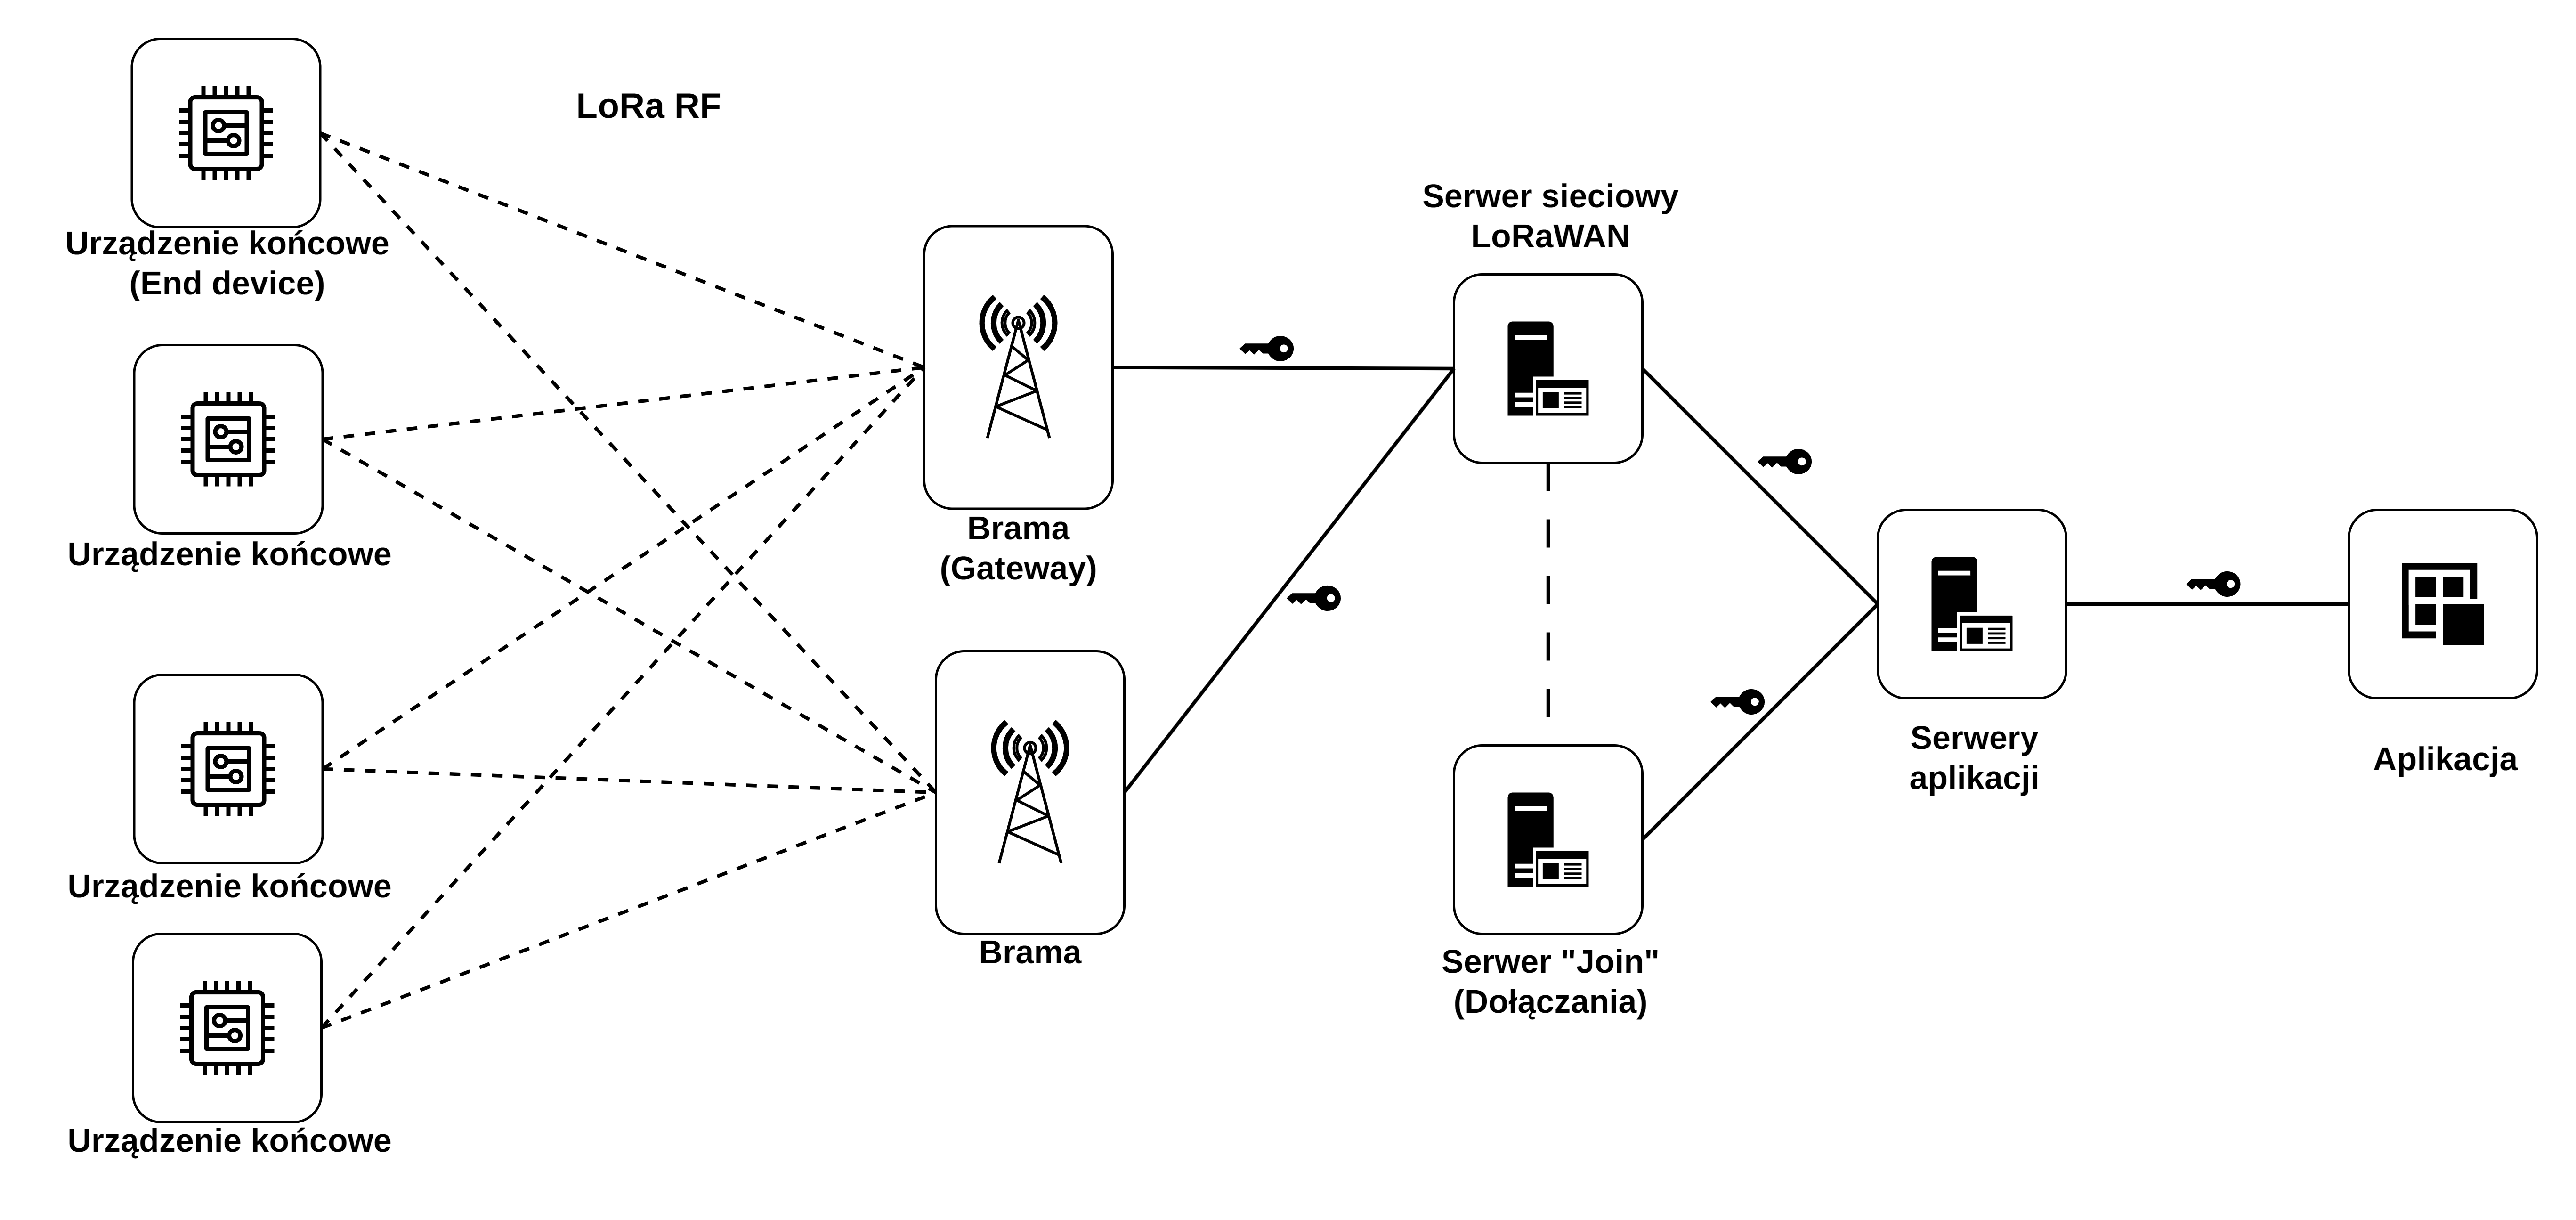
\includegraphics[width=\textwidth]{schematics/lorawan-architecture}
    \caption{\label{img:lorawan-architecture}Schemat architektury sieci LoRaWAN}
\end{figure}

\chapter{\label{ch:development}Platforma sprzętowa oraz przygotowanie środowiska programistycznego}
Oprogramowanie wszystkich elementów zostało napisane z~wykorzystaniem PlatformIO. Narzędzie pozwala na budowanie pod
systemy wbudowane na wiele platform \cite{pio-platforms}, w~tym wykorzystane do zbudowania sieci STMicroelectronics
STM32 Nucleo. Do kompilacji kodu źródłowego możliwe jest użycie wtyczki do edytora Visual Studio Code
\enquote{PlatformIO IDE} lub samodzielnego narzędzia CLI (ang. \textsl{Command Line Interface}) \enquote{PlatformIO
    Core}.

Rozwiązanie to zostało wybrane jako główne narzędzie do kompilacji oraz wgrywania kodu źródłowego, z~uwagi na to, że
działa na wielu plaformach. Dzięki temu nie jest wymagane instalowanie oraz ustawianie osobnych, dedykowanych środowisk
dla każdej z~wykorzystywanych platform. Jedynym wymogiem, aby móc zacząć pracę jest zainicjowanie projektu oraz
ustawienie podstawowej konfiguracji. Zadanie to jest bardzo proste, ponieważ dokumentacja narzędzia jest rozbudowana
i~bardzo szczegółowa.

\section{Rozpoczęcie projektu z~PlatformIO Core\label{sect:pio-intro}} Całość sieci składa się z~dwóch oddzielnych
projektów -- pierwszy z~nich to projekt uniwersalny dla modułów MASTER oraz SLAVE sieci LoRa, drugi natomiast
wykorzystywany jest do mikrokontrolera Adafruit Feather M0. Aby rozpocząć nowy projekt, należy wykorzystać komendę,
gdzie argumentem jest docelowy mikrokontroler:
\begin{verbatim}
   pio project init --board <board>
\end{verbatim}

W przypadku projektu dla sieci LoRa wykorzystane zostały płytki Nucleo L152RE, stąd argumentem było
\texttt{nucleo\_l152}, natomiast dla projektu serwera sieci lokalnej -- \texttt{adafruit\_feather\_m0}. Użycie komendy
rozpoczyna proces tworzenia nowego projektu. Na podstawie podanego argumentu tworzony jest plik konfiguracyjny.
Zdefiniowane zostają platforma projektu oraz wykorzystywany framework. W~przypadku obu projektów wybrany został ten
wykorzystywany przez Arduino z~uwagi na dużą dostępność bibliotek, które działają bez potrzeby modyfikowania ich kodu
źródłowego. Dodatkowo zdefiniowana została tutaj prędkość transmisji portu szeregowego.

W projekcie dla modułów sieci wykonana została modyfikacja pliku konfiguracyjnego -- elementy wygenerowane przez
narzędzie CLI PlatformIO przeniesione zostały do osobnej sekcji \texttt{[base\_config]}, natomiast konfiguracje dla
poszczególnych modułów znajdują się w~dedykowanych \enquote{środowiskach}. Wprowadzone zmiany zostały dokładniej opisane
w sekcjach o~implementacji oprogramowania na poszczególne moduły (\ref{sect:firmware-network},
\ref{sect:firmware-webserver}).

Poza plikiem konfiguracyjnym, narzędzie generuje też podstawową strukturę plików całego. Powstaje folder \texttt{src},
który dedykowany jest dla plików źródłowych, \texttt{include} dla plików nagłówkowych, \texttt{lib} dla bibliotek
lokalnych oraz \texttt{tests} do testów jednostkowych, jeżeli planowane jest użycie ich.

\section{Praca z~PlatformIO\label{sect:pio-work}} Po stworzeniu projektu możliwe jest przystąpienie do pisania kodu
źródłowego na wybraną platformę. PlatformIO udostępnia możliwość kompilowania kodu oraz wgrywania go na docelowe
urządzenie poprzez jedną jedną komendę lub jeden przycisk w~edytorze tekstu. Jest to bardzo dobre rozwiązanie,
ponieważ dzięki temu możliwe jest skupienie się na rozwoju kodu źródłowego, zamiast czekania aż projekt będzie możliwy
do uruchomienia i~sprawdzenia.

\subsection{Uruchamianie projektu\label{sect:pio-run}} Uruchomienie projektu jest w~przypadku PlatformIO rozumiane
poprzez wykonanie kompilacji (\texttt{build}), wgranie skompilowanego kodu na urządzenie docelowe (\texttt{upload}) lub
wykonanie zdefiniowanego zestawu testów jednostkowych (\texttt{test}). Aby uruchomić projekt należy wykorzystać komendę:
\begin{verbatim}
   pio run [OPTIONS]
\end{verbatim}
Argumentami dodatkowymi mogą być:
\begin{itemize}[label=]
    \item \texttt{--environment}: element konfiguracji projektu, który określa zależności w~kwestiach
          kompilacji (np. flagi budowania projektu), programowania (wgrywania kodu) docelowych urządzeń, testów
          jednostkowych lub wykorzystanych bibliotek,
    \item \texttt{--target}: cel uruchomienia (np. kompilacja albo kombinacja kilku celów jednocześnie),
    \item \texttt{--upload-port}: port, do którego podłączone jest urządzenie i~na które ma zosatać wgrany kod.
          Szczególnie użyteczne w~przypadku, gdy pracuje się na wielu urządzeniach jednocześnie,
    \item \texttt{--monitor-port}: port, na którym po zakończeniu procesu ma zostać otwarty monitor portu szeregowego.
\end{itemize}
W przypadku opcji związanych z~portem, jeżeli nie zostaną sprecyzowane (podane jako argument do komendy), PlatformIO
będzie próbował wykryć je automatycznie. Dostępne jest jeszcze kilka innych opcji, jednkże są one znacznie rzadziej
wykorzystywane, ponieważ ich domyślne opcje są tymi, które są najczęściej ustawiane.

\subsection{Zarządzanie bibliotekami\label{sect:pio-pkg}} PlatformIO posiada wbudowany moduł dedykowany do zarządzania
bibliotekami oraz innymi zasobami dołączanymi do projektu. Dzięki wykorzystaniu odpowiedniej podkomendy z~zestawu:
\begin{verbatim}
   pio pkg [COMMAND]
\end{verbatim}
możliwe jest przeszukiwanie, instalowanie z, aktualizacja lub publikowanie do rejestru dostępnych bibliotek. Podczas
wyszukiwania możliwe jest też zastosowanie filtrów, które w~znacznym stopniu zmniejszają ilość wyników i~przybliżają do
znalezienia tego pasującego. Wykorzysując tę operację zainstalowane zostały potrzebne do projektów biblioteki (wbudowane
dla frameworku Arduino, tak jak \enquote{Wire} czy te, które opublikowane zostały na platformie GitHub i~dodane do
rejestru PlatformIO). Na rys. \ref{img:pio-pkg-search} przedstawiony zostały przykładowy wynik wyszukiwania dostępnych
bibliotek związanych z~hasłem \enquote{LoRa}. Każdy wynik zawiera informację: nazwę, typ paczki, biblioteki, która
została znaleziona, najnowszą wersję, datę publikacji oraz krótki opis tego czym dana paczka, biblioteka są. Komenda
pokazuje także informacje o~tym ile wyników zostało znalezionych.

\begin{figure}[!htbp]
    \centering
    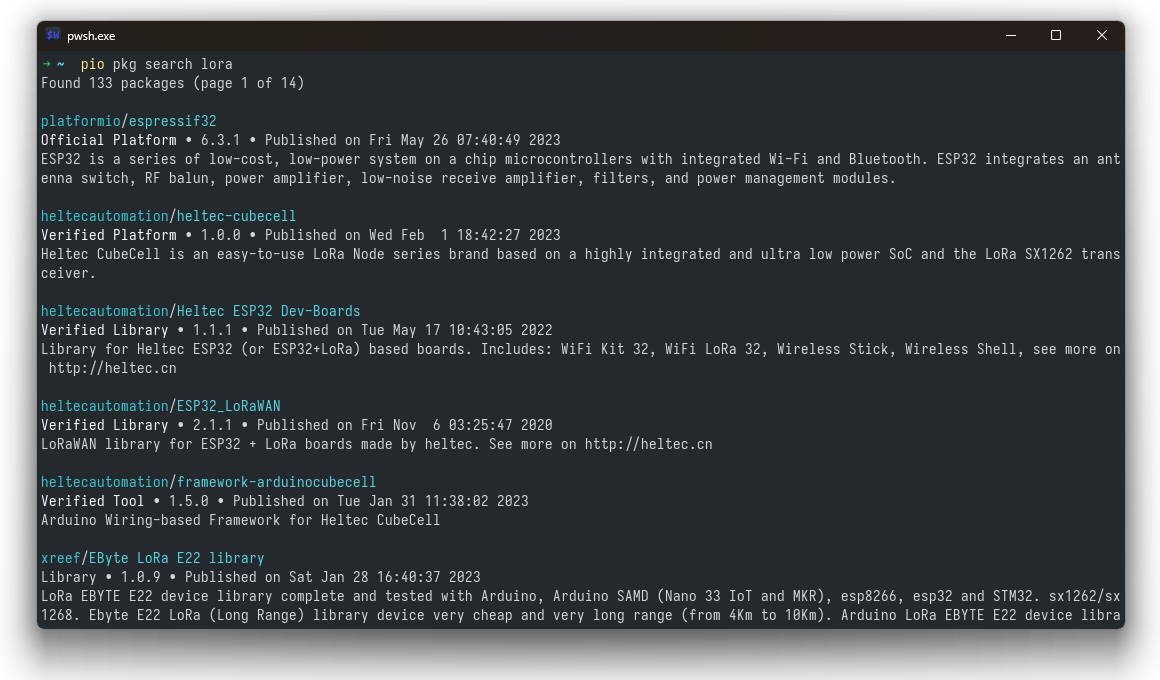
\includegraphics[width=1.0\textwidth]{screenshots/pio-pkg-search}
    \caption{\label{img:pio-pkg-search}Wyniki wyszukiwania bibliotek powiązanych z~hasłem \enquote{LoRa}}
\end{figure}

\chapter{\label{ch:implementation}Implementacja oprogramowania}
Całość oprogramowania wykorzystuje język programowania \texttt{C++}. Projektowana oraz implementowana sieć składa się
z~dwóch typów modułów, stąd też pojawiła się potrzeba zainicjowania dwóch osobnych projektów -- jednego pod elementy
sieci LoRa oraz drugiego, dedykowanego dla modułu serwera sieciowego (ang. \textsl{webserver}), z~uwagi na zupełnie inną
platformę sprzętową. Firmware napisany został z~wykorzystaniem kilku różnych podejść:
\begin{itemize}[label=--]
    \item modułowego: każdy plik źródłowy odpowiada za zbiór funkcji wykonujących określone zadania (np. praca
          z~biblioteką do modułów LoRa zaimplementowana jest w~pliku \texttt{lora.cpp}),
    \item obiektowego: większość elementów kodu źródłowego jest reprezentowana w~postaci osobnego obiektu. Każdy
          z~nich posiada swoje funkcje oraz pełni określone zadania (np. obiekt \enquote{\texttt{bme}} ma za zadanie
          umożliwić współpracę z~sensorami dostępnymi na płytce czujników BME280, która podłączona jest do każdego
          modułu SLAVE).
\end{itemize}
Ponadto, wykorzystane zostały elementy języka \texttt{C++}, które dostępne są w~nowszych wersjach -- funkcje szablonowe
(ang. \textsl{template functions}) lub pętle typu \texttt{for-range}. Są to elementy, które znacznie ułatwiły
implementację kodu oraz pozwoliły na minimalizację powtarzalności pewnych elementów.

Z uwagi na zastosowanie podejścia modułowego, całość oprogramowania składa się z~wielu mniejszych elementów,
podzielonych na odpowiadające im pliki. Aby mieć pewność, że implementowane funkcje nie będą posiadały żadnych kolizji
w~swoich nazwach zastosowane zostały przestrzenie nazw (ang. \textsl{namespaces}). Dodatkowo, ponieważ kod źródłowy
jest dostępny w~domenie publicznej (repozytorium na platformie GitHub z~licencją \textsl{MIT} \cite{snyk-sw-license}),
podjęta została decyzja o~dodaniu opisów działania do wszystkich elementów. Wykorzystany został do tego \textsl{Doxygen}
-- narzędzie do generowania dokumentacji (np. formie strony internetowej lub dokumentu w~\LaTeX) na podstawie
specjalnych znaczników w~komentarzach \cite{doxygen}.

\section{Framework oraz biblioteki\label{sect:framework-libraries}} Bazą do oprogramowania na wszystkich modułach jest
framework Arduino oraz jego modyfikacja pod platformę STM32 -- stm32duino, która pozwala na wykorzystanie pełnej
funkcjonalności rdzenia Arduino \cite{stm32duino-docs}. Pomimo tego, że biblioteki HAL (ang. \textsl{Hardware
    Abstraction Layer}) oraz framework STM32 są narzędziami dedykowanymi, w~przypadku tego projektu nie można było ich
zastosować. Oryginalna biblioteka do obsługi modułów rozszerzeń LoRa została wycofana z~użytku na rzecz nowszej
implementacji, pod nowszą wersję płytek Nucleo z~wbudowanym hardware.

\subsection{Wykorzystane biblioteki\label{sect:used-libs}} Do implementacji oprogramowania na wszystkie moduły
wykorzystanych zostało kilka bibliotek, które pozwalały na dodanie pełnego zakresu funkcjonalności do każdego
z~projektów.

W przypadku bibliotek zewnętrznych (niebędących częścią rdzenia Arduino) były to:
\begin{itemize}[label=--]
    \item STM32duino I-NUCLEO-LRWAN1: biblioteka do uruchomienia oraz pracy z~modułem rozszerzeń LoRa. Pozwala ona na
          pracę w~dwóch trybach: LoRaRadio -- implementacja wykorzystująca tylko standard dolnej warstwy sprzętowej LoRa
          oraz LoRaWAN -- dodająca możliwość podłączenia modułów do istniejącej sieci LoRa oraz wysyłanie i~odbieranie
          z~niej wiadomości,
    \item Adafruit BME280 Library: biblioteka dedykowana do modułów BME280, pozwalająca na zbieranie danych z~sensorów,
          wykorzystując do tego magistralę SPI albo I2C (w~zależności od posiadanego modułu rozszerzeń),
    \item Adafruit BusIO: uniwersalna biblioteka dodająca pewien poziom abstrakcji do komunikacji po magistralach I2C
          oraz SPI,
    \item WiFi101: biblioteka, która daje możliwość wykorzystania modułu WiFi obecnego na płytce Adafruit Feather M0
          (wykorzystanej do uruchomienia serwera w~sieci lokalnej).
\end{itemize}
Ponadto, wykorzystane zostały biblioteki I2C oraz SPI, dostępne w~rdzeniu Arduino. Potrzebne były one do uzyskania
komunikacji pomiędzy mikrokontrolerem Adafruit Feather M0 a~modułem WiFi, sensorami BM280 podłączonymi do modułów SLAVE
oraz do stworzenia połączenia pomiędzy modułem MASTER a~płytką z~serwerem sieci lokalnej.

\subsection{Ograniczenia związane z~wykorzystaniem Arduino oraz STM32duino\label{sect:framework-limits}} STM32duino,
pomimo tego, że ułatwił, bądź w~ogóle pozwolił na pracowanie z~wykorzystywanymi modułami, nie jest platformą idealną,
pozbawioną ograniczeń. Jedynym z~nich, które w~dość znacznym stopniu utrudniło implementację oprogramowania dla modułów
sieci, był brak przerwań programowych oraz ograniczone możliwości zastosowania przerwań sprzętowych. Stąd też pojawił
się wymóg zastosowania pewnych obejść, jednocześnie tracąc na wydajności implementowanego rozwiązania. Ponadto,
występowały też problemy związane z~działaniem magistrali I2C, tutaj w~przypadku modułów Feather oraz standardowego
Arduino -- niemożliwe było wykorzystanie wyświetlacza OLED pracującego na magistrali I2C oraz zarejestrowania samego
mikrokontrolera jako części, z~którą można komunikować się po tej magistrali.

\section{Implementacja oprogramowania elementów sieci\label{sect:firmware-network}} Zaprojektowana sieć składała się
w~sumie z~pięciu modułów -- 4~z~nich stanowiły elementy sieci LoRa, natomiast ostatni był wykorzystywany jako serwer
w~sieci lokalnej. W~projekcie nie została wykorzystana pełna funkcjonalność LoRaWAN oraz typowa dla niej architektura
(przedstawiona w~sekcji \ref{sect:lorawan}, rys. \ref{img:lorawan-architecture}), ponieważ implementacja takiego
rozwiązania jest bardzo kosztowna i~wymaga znacznie większej ilości elementów. Aby móc skorzystać ze specyfikacji
wymagane jest posiadanie bramy (ang. \textsl{gateway}) oraz serwerów odpowiedzialnych za przyłączanie urządzeń,
zarządzanie siecią oraz serwera aplikacyjnego. Z~uwagi na to zastosowana została dużo prostsza i~mniej wymagająca metoda
budowania sieci, opierająca się na wykorzystaniu modułów w~formie nadajników radiowych, pracujących w~standardzie LoRa.
Schemat ideowy budowanej sieci przedstawiony został na rys. \ref{img:network-schematic}.

\begin{figure}[!htbp]
    \centering
    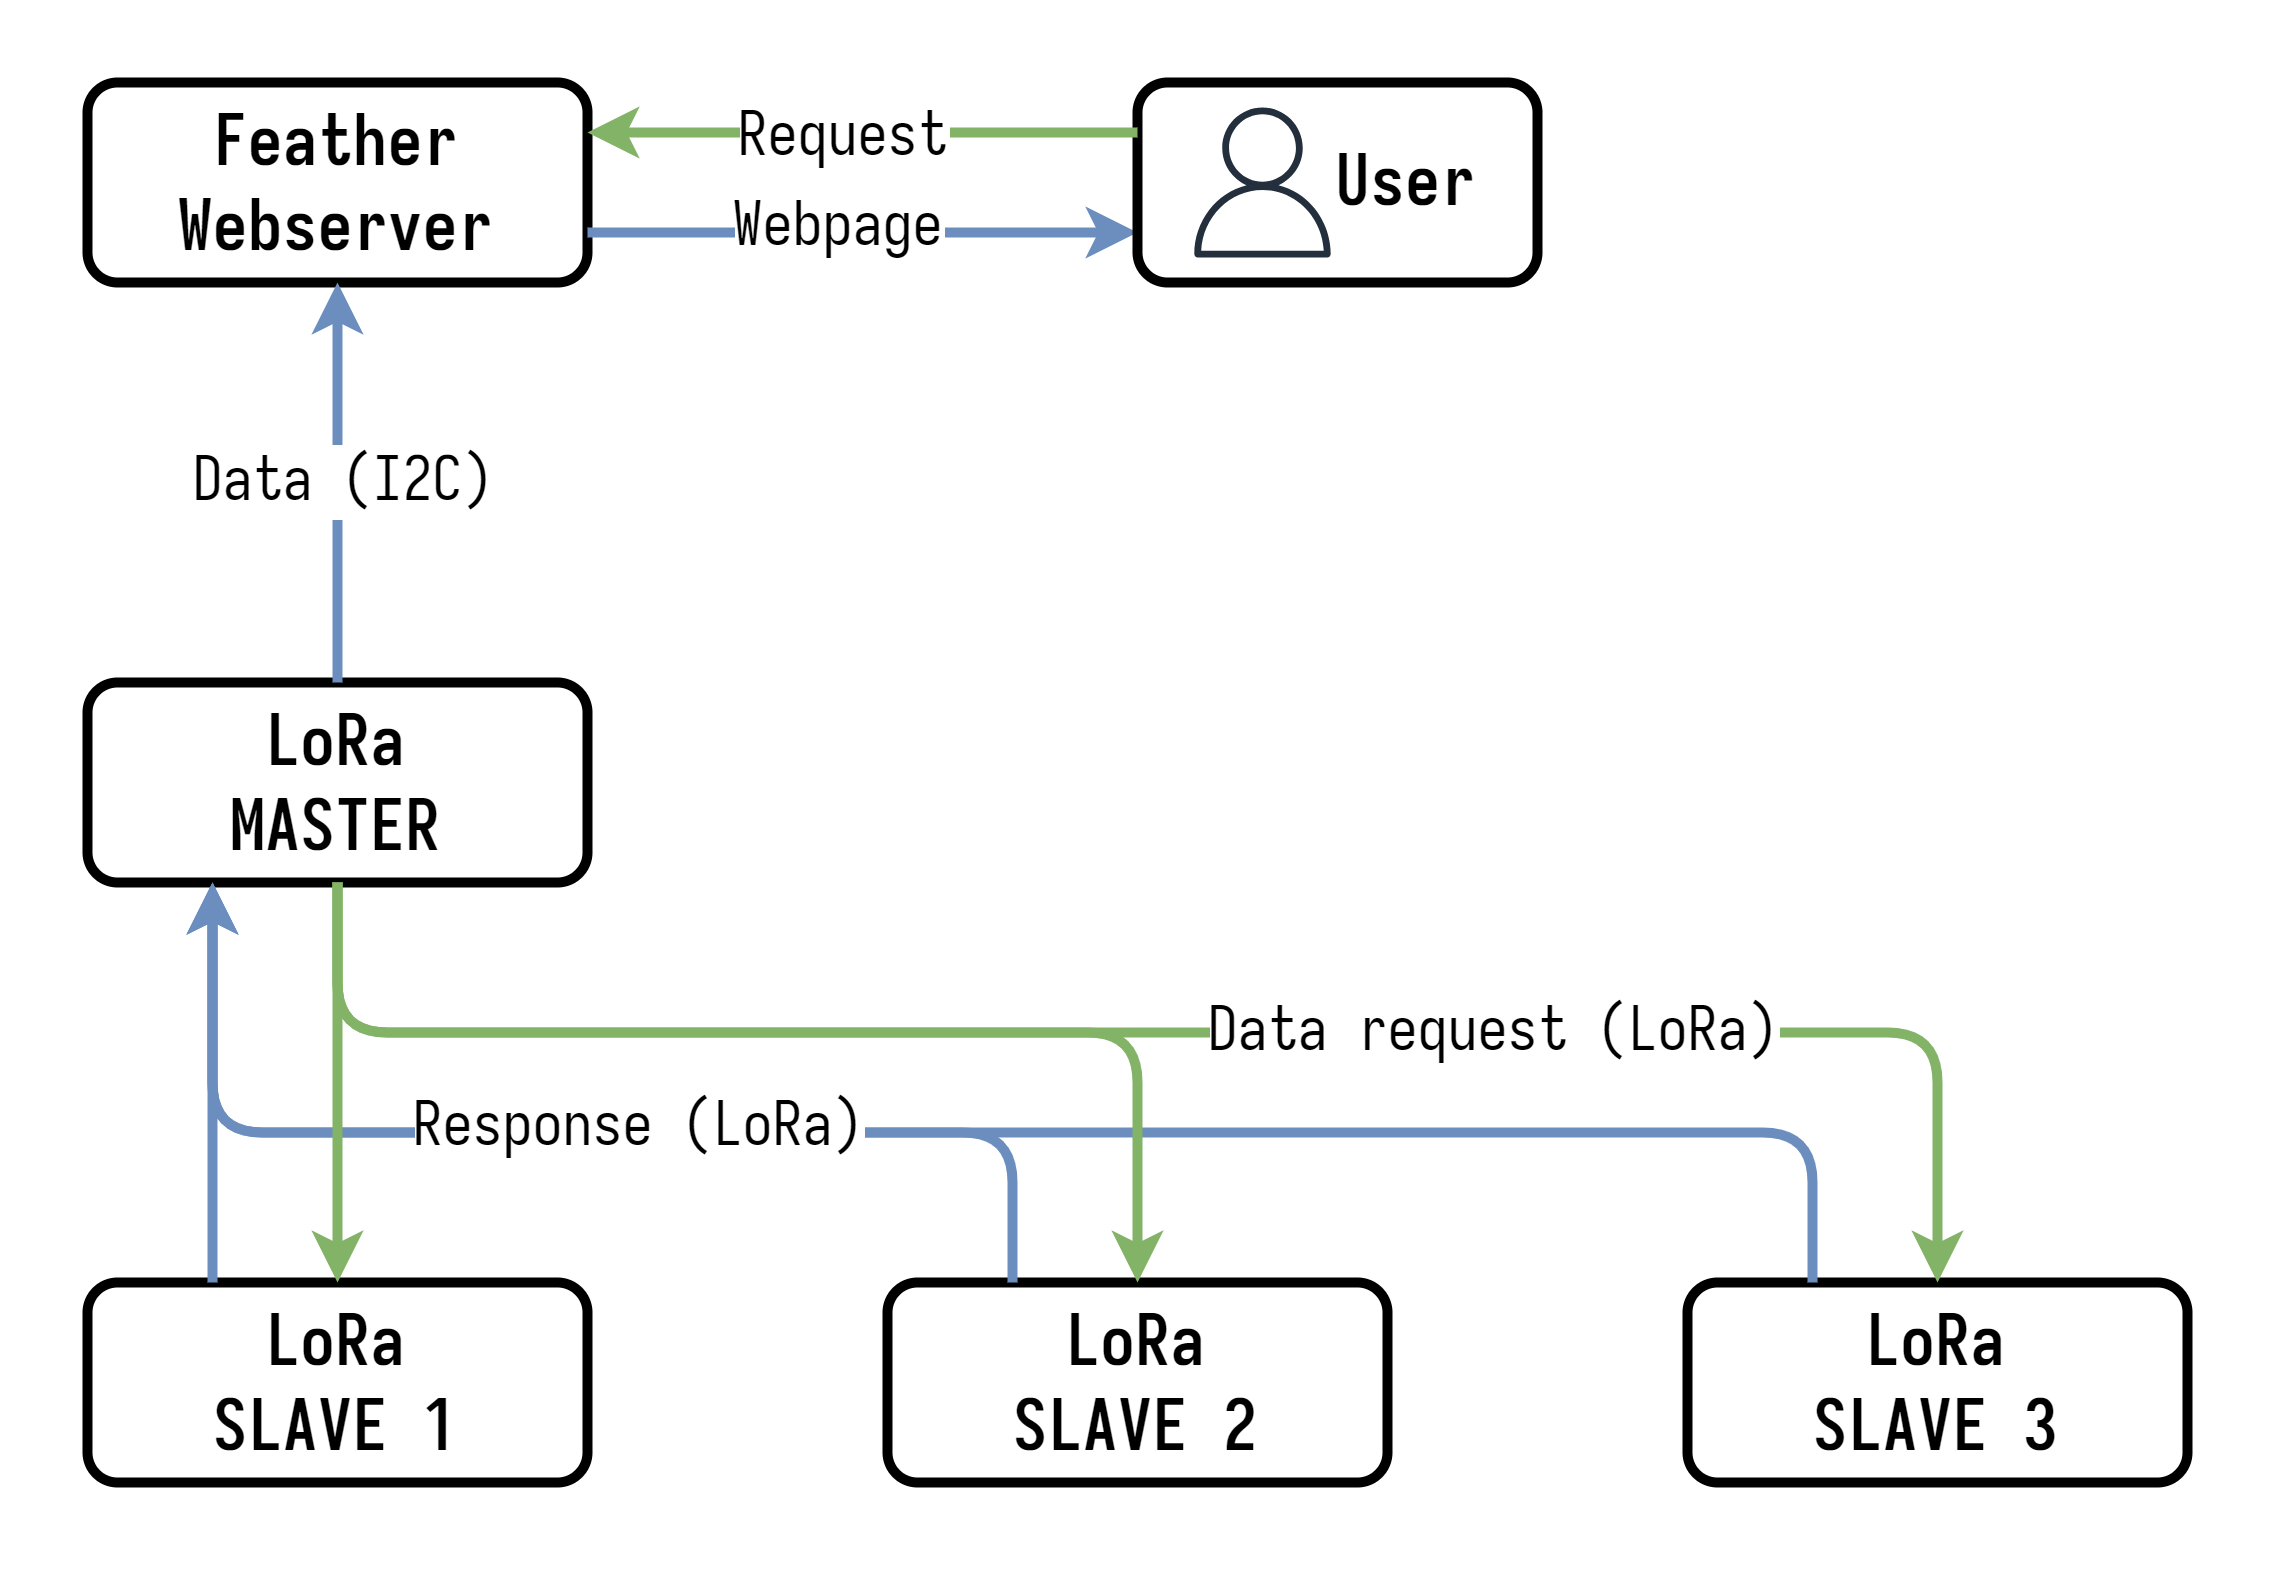
\includegraphics[width=0.8\textwidth]{lora-psn/images/network-schematic}
    \caption{\label{img:network-schematic}Schemat zbudowanej sieci, z~oznaczonymi elementami komunikacji}
\end{figure}

Oprogramowanie dla modułów pracujących w~sieci LoRa zostało zaimplementowane w~formie uniwersalnej -- jeden projekt
zawiera elementy dla modułu MASTER oraz modułów SLAVE. Plik konfiguracyjny projektu zawiera flagę, która definiuje, na
jaki typ modułu kod zostanie skompilowany. Co więcej, w~przypadku modułów SLAVE dodana została też flaga informująca
o~tym, jakie ID przypisane zostaje danej płytce. Rozwiązanie to odgrywa znaczącą rolę w~tym, jak wiadomości są
przesyłane w~sieci. Fragment pliku konfiguracyjnego, który odpowiedzialny jest za definiowanie tych elementów
przedstawiony został na listingu \ref{lst:lora-ini}.

\lstinputlisting[
    linerange={26-30},
    caption={Fragment pliku konfiguracyjnego (tutaj dla SLAVE1) odpowiedzialny za definicję typu oraz ID modułu},
    label={lst:lora-ini}
]{lora-psn/platformio.ini}

Wykorzystanie frameworku Arduino wymagało zastosowania pewnych schematów podczas implementacji. Dlatego też całość kodu
podzielona jest na dwie sekcje \texttt{setup()} oraz \texttt{loop()}, wykonywane odpowiednio raz, podczas startu modułu
oraz w~nieskończonej pętli, dopóki płytka ma zasilanie. Na rys. \ref{img:firmware-flowchart} przedstawiony został
schemat blokowy zaimplementowanego oprogramowania -- części zawartej w~sekcji \texttt{setup()}.

\begin{figure}[!htbp]
    \centering
    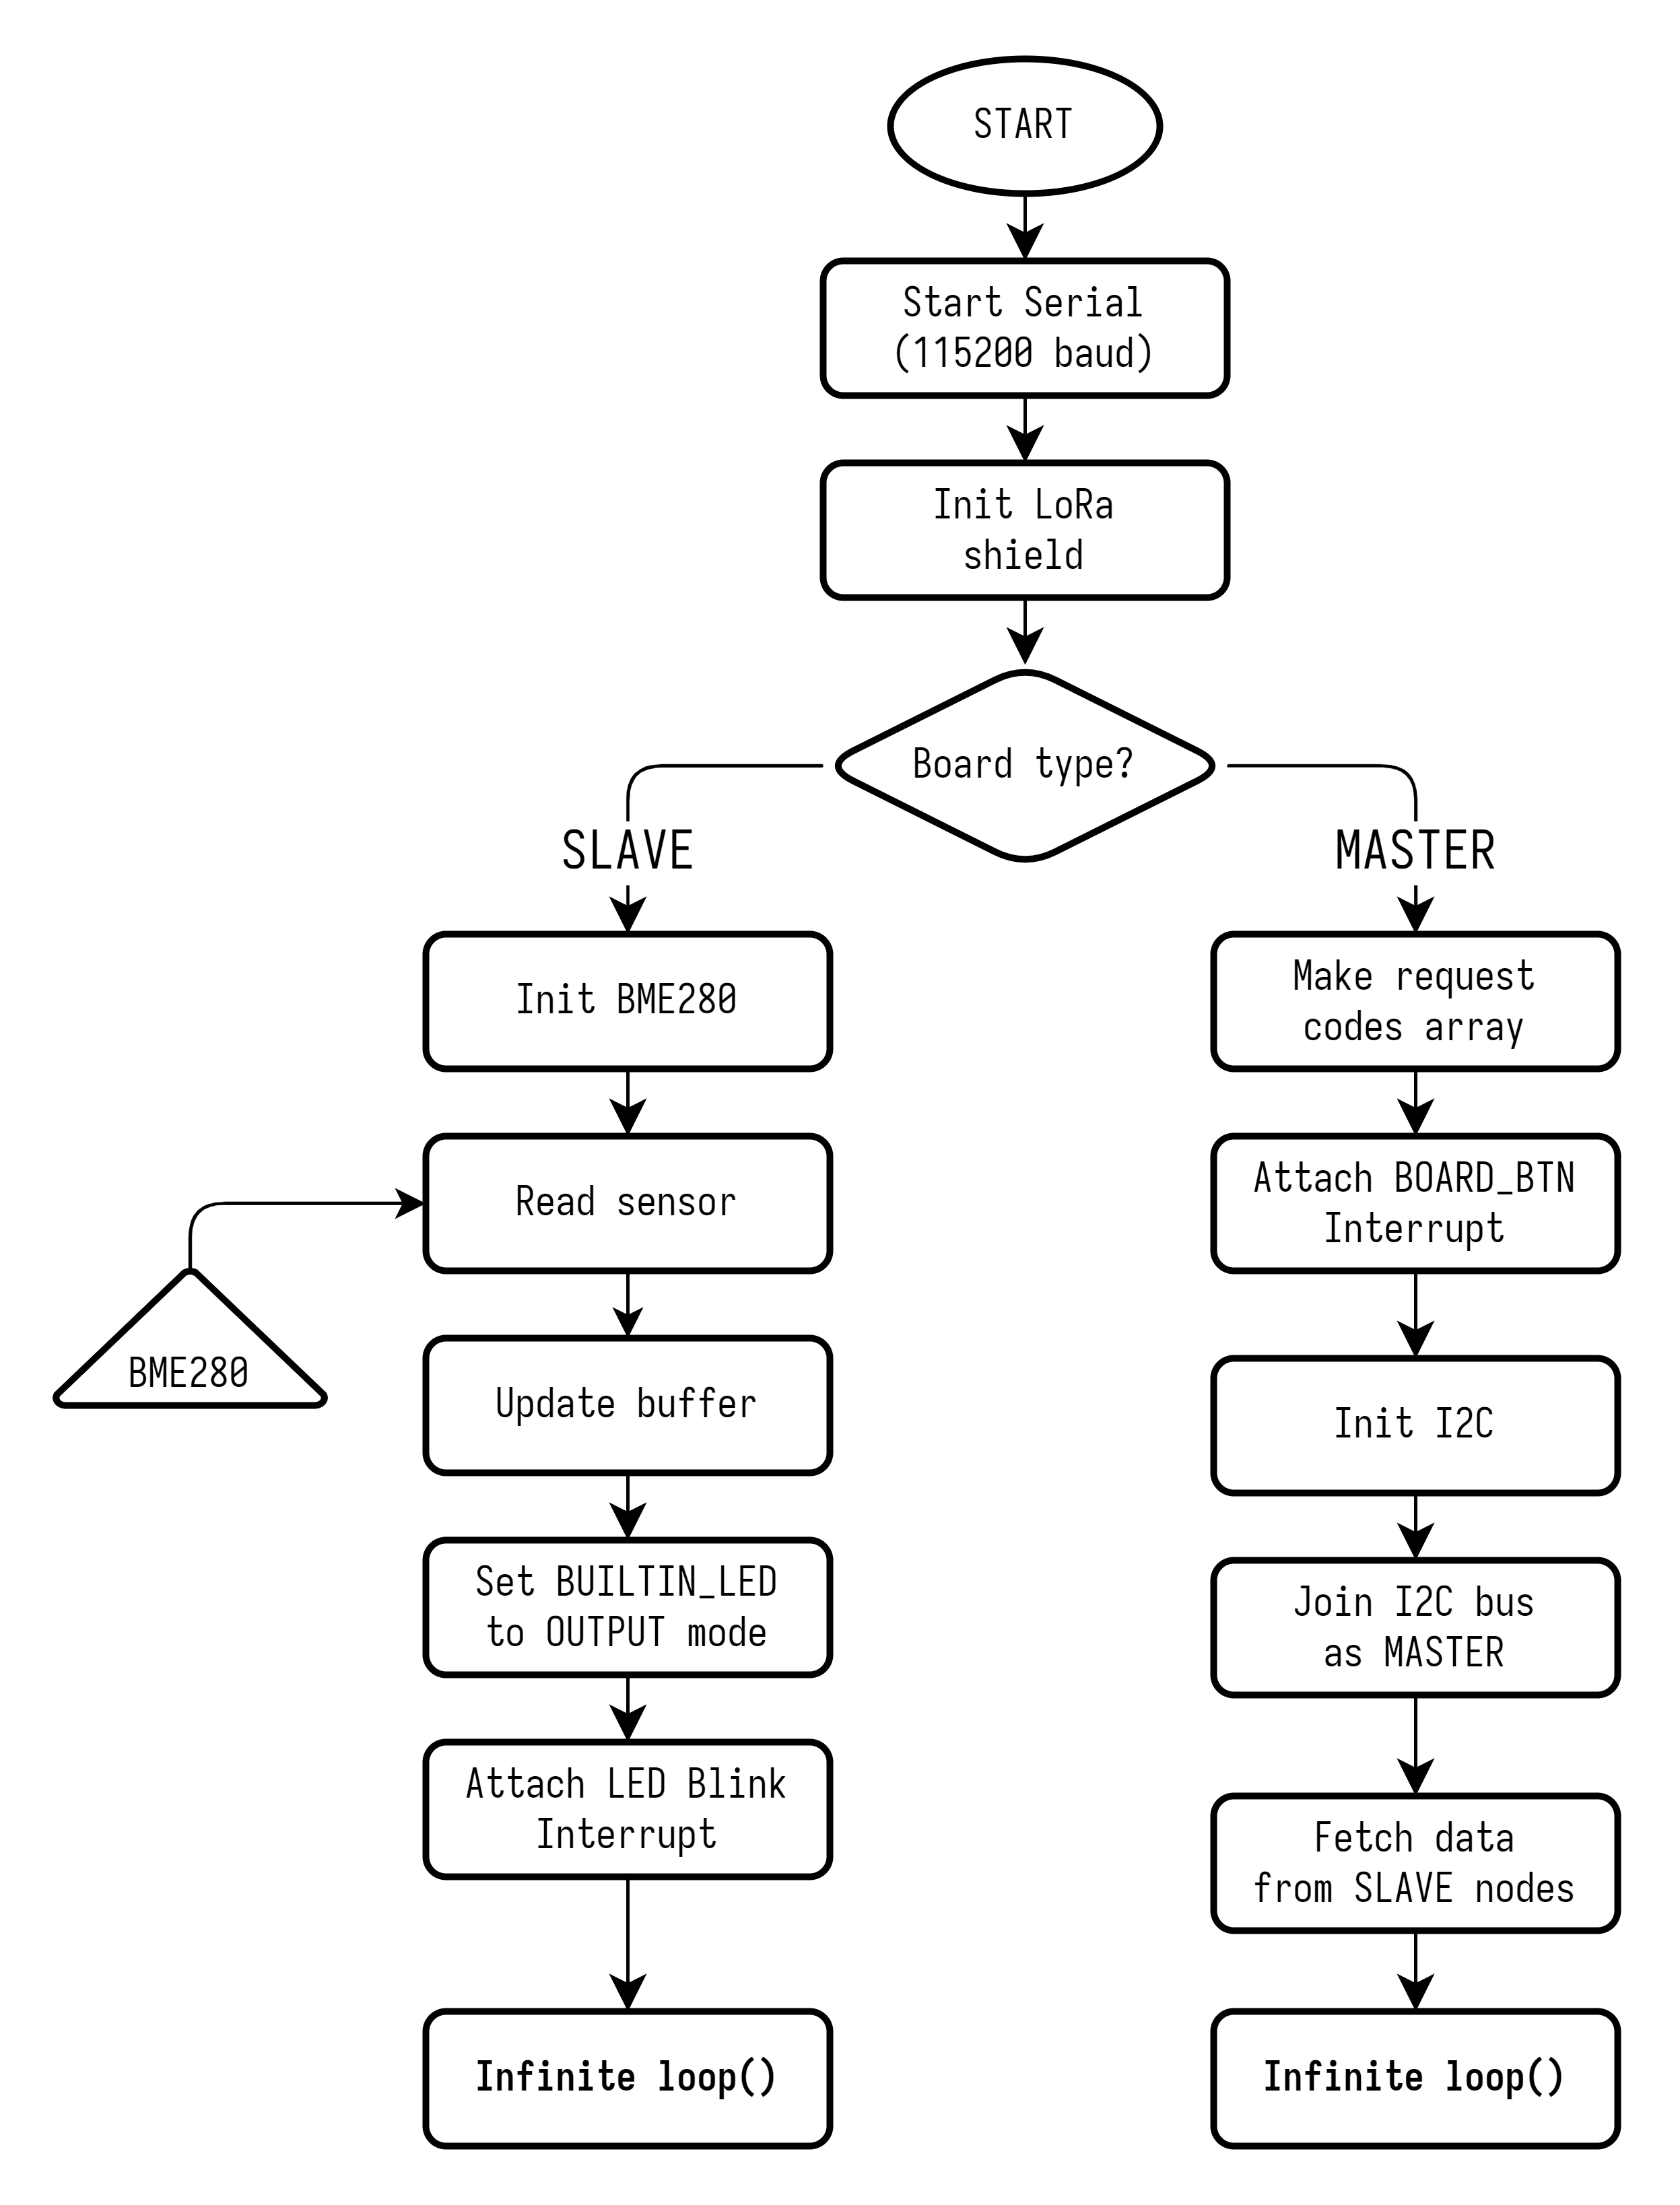
\includegraphics[width=0.9\textwidth]{lora-psn/images/firmware-flowchart}
    \caption{\label{img:firmware-flowchart}Schemat blokowy części \texttt{setup()} oprogramowania modułów sieci LoRa,
        z~podziałem na typ płytki}
\end{figure}

Oba typy oprogramowania zaczynają od ustawienia portu szeregowego na 115200 baud (szybkość transmisji), następnie
inicjowane jest rozszerzenie LoRa. Logowana jest informacja o~typie płytki, a~następnie kod oczekuje na informacje
o~starcie modułu rozszerzenia. W~przypadku błędu oraz poprawnego startu na port szeregowy wystawiana jest odpowiednia
informacja.

Następnie, w~zależności od typu płytki, wykonywane jest kilka operacji. W~przypadku modułów SLAVE są to:
\begin{enumerate}
    \item przygotowanie sensora BME280 oraz pobranie z~niego danych,
    \item aktualizacja zawartości bufora (wykorzystywanego do przechowywania odczytanych wartości),
    \item przygotowanie diody LED, która informuje o~trwającej komunikacji w~sieci,
    \item przygotowanie przerwania, wykorzystywanego do obsługi nowych zapytań.
\end{enumerate}

Natomiast dla modułów MASTER wykonywany jest inny zestaw operacji, z~uwagi na to, że taki moduł pełni zupełnie inną
funkcję w~sieci:
\begin{enumerate}
    \item przygotowanie tablicy z \enquote{kodami} zapytań (jedno bajtowe wartości do określenia czego żąda MASTER),
    \item inicjacja magistrali I2C i~podłączenie modułu jako MASTER,
    \item wykonanie podprogramu wysyłającego zapytania oraz odbierającego odpowiedzi od SLAVE-ów, tak aby tuż po
          starcie można było odczytać dane z~sieci.
\end{enumerate}
Ostatnim krokiem w~obu przypadkach jest przejście do nieskończonej pętli i~wykonywanie instrukcji w~niej zawartych,
wykorzystując do tego określony okres zegara.

Dodatkowo, oprogramowanie posiada zestaw definicji oraz funkcji wykorzystywanych do debugowania, które ułatwiały
implementację oprogramowania -- \texttt{globals.h} oraz \texttt{debug.h}. Najważniejszymi elementami pliku globalnych
definicji są funkcje preprocesora -- zwracających tylko ID modułu lub ID danej na podstawie kodu zapytania oraz
struktury szablonowe (ang. \textsl{template structures}), które zawierają informację o~tym jaki kształt powinny mieć
dane zbierane z~sensorów oraz przekazywane przez sieć. Definicję przedstawiono na listingu \ref{lst:globals}, natomiast
dla funkcji wysłającej sformatowane wiadomości przez port szeregowy na listingu \ref{lst:debug}. Implementacja oparta
została o~funkcję z~rdzeniu Arduino -- \texttt{Serial.println()}.

\lstinputlisting[
    language=C++,
    linerange={6-8,15-39},
    caption={Definicje funkcji dla preprocesora oraz struktury szablonowe (z polami o~jednej wartości oraz z~tablicami)},
    label={lst:globals},
]{lora-psn/include/globals.h}

\lstinputlisting[
    language=C++,
    linerange={20-26},
    caption={Funkcji wykorzystywana do wysyłania sformatowanych wiadomości przez port szeregowy},
    label={lst:debug},
]{lora-psn/include/debug.h}

\FloatBarrier
\subsection{Oprogramowanie modułu MASTER\label{sect:firmware-master}} Po wykonaniu instrukcji, które
opisane zostały w~poprzedniej sekcji, moduł MASTER przechodzi do pracy w~nieskończonej pętli -- \texttt{loop()}.
Wszystko oparte jest na zegarze o~zdefiniowanym okresie -- wybrana została wartość 1~minuty (60000 milisekund).
Implementacja oparta została o~zegar nieblokujący (ang. \textsl{non-blocking timer}) z~wykorzystaniem funkcji
\texttt{millis()} -- funkcji zwracającej ilość milisekund od momentu startu programu. Okres został zdefiniowany
w~definicjach preprocesora, w~celu uniknięcia tzw. magicznych liczb (ang. \textsl{magic numbers}).

W momencie, gdy mija wymagany czas, program przechodzi do wykonania podprogramu odpowiadającego za wysyłanie zapytań
oraz zbieranie odpowiedzi z~sieci. Na rys. \ref{img:master-flowchart} przedstawiony został diagram blokowy instrukcji
wykonywanych przez moduł MASTER w~nieskończonej pętli oraz tego, co wykonywane jest w~podprogramie komunikacji.
Natomiast pełna implementacja obu tych elementów przedstawiona została na listingach \ref{lst:main-loop} oraz
\ref{lst:master-fetch}.

\begin{figure}[!htbp]
    \centering
    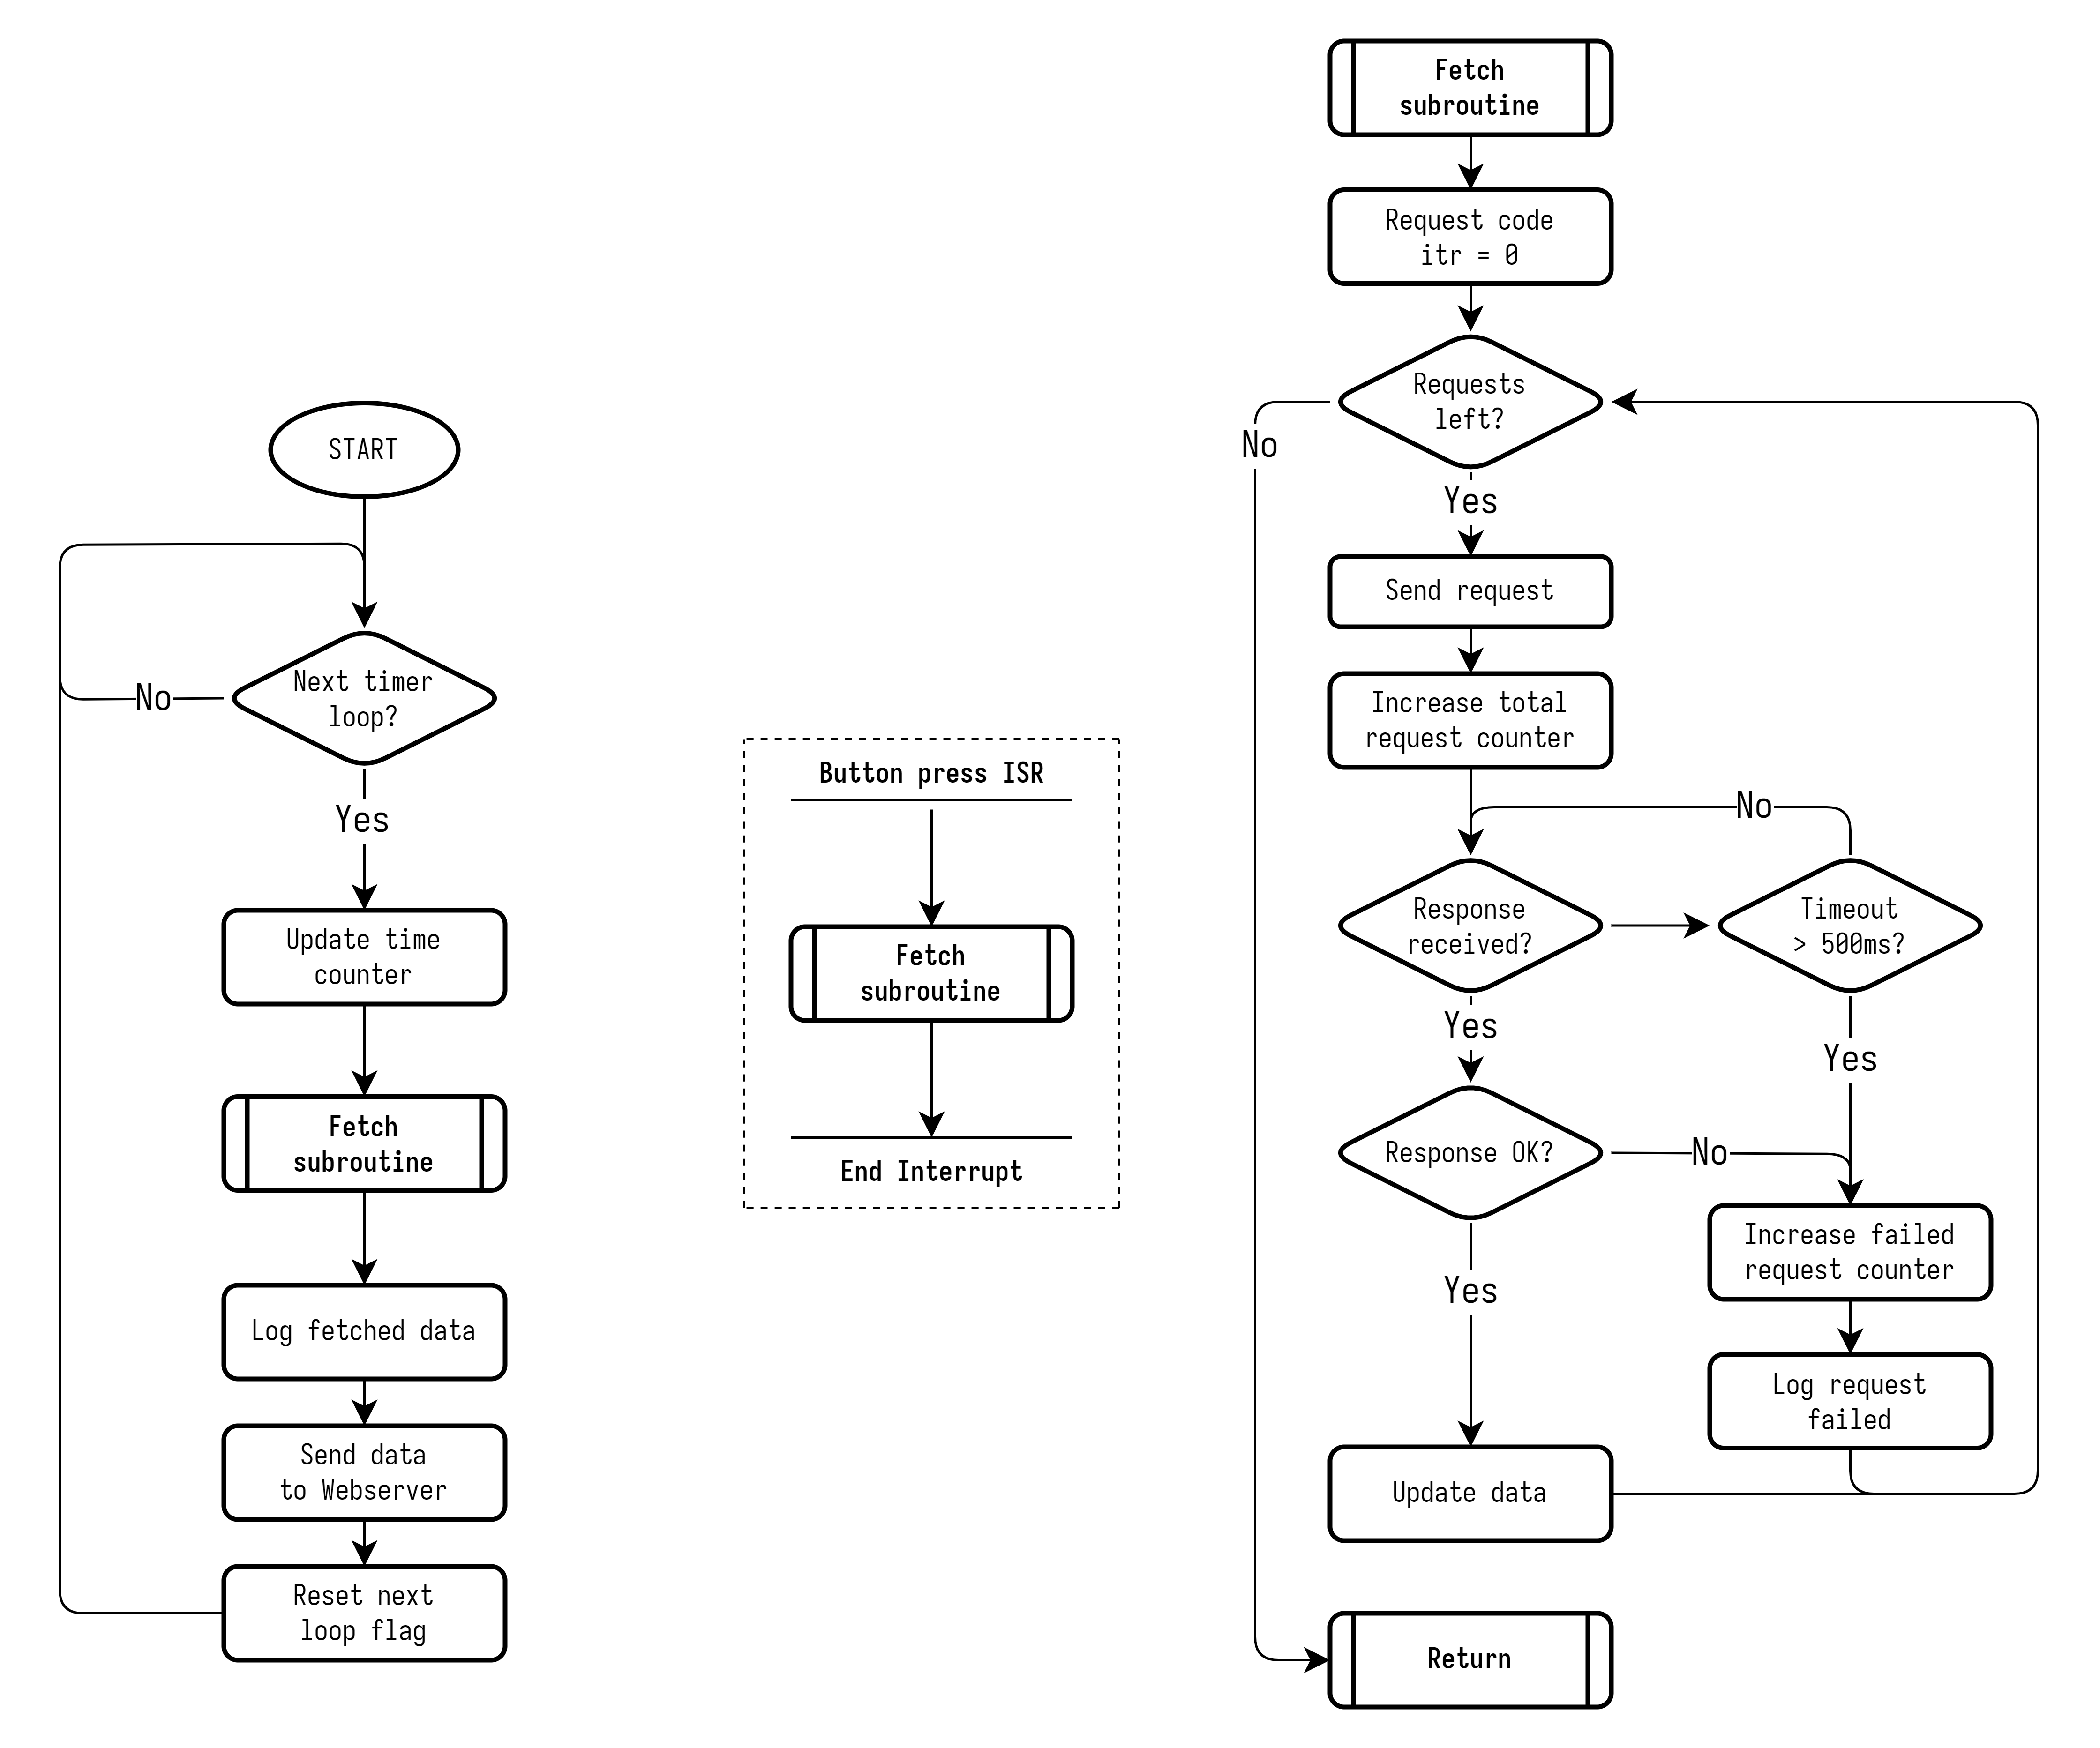
\includegraphics[width=0.9\textwidth]{lora-psn/images/MASTER-loop-flowchart}
    \caption{\label{img:master-flowchart}Schemat blokowy nieskończonej pętli oraz podprogramu zbierania danych
        zaimplementowanych dla modułu MASTER}
\end{figure}

\lstinputlisting[
    language=C++,
    linerange={103-110,112-116},
    caption={Implementacja nieskończonej pętli dla modułu MASTER},
    label={lst:main-loop},
]{lora-psn/src/main.cpp}

\lstinputlisting[
    language=C++,
    linerange={133-174},
    caption={Funkcja podprogramu odpowiedzialnego za zbieranie danych w~sieci},
    label={lst:master-fetch},
]{lora-psn/src/main.cpp}

Pierwszym elementem podprogramu jest wysłanie nowego zapytania do sieci -- zaimplementowana została do tego funkcja
\texttt{sendRequest()} zawarta w~przestrzeni nazw \texttt{lora}. Jej implementacja przedstawiona została na listingu
\ref{lst:lora-sendrequest}. Pobierany jest kod, który ma zostać wysłany do sieci, następnie, wykorzystując funkcję
\texttt{debug::println()} logowana jest przesyłana wartość. Korzystając z~funkcji, która dostępna jest w~bibliotece do
obsługi modułu rozszerzeń LoRa, wysyłana jest wiadmość do sieci.

\lstinputlisting[
    language=C++,
    linerange={37-43},
    caption={Implementacja funkcji \texttt{lora::sendRequest()}},
    label={lst:lora-sendrequest},
]{lora-psn/src/lora.cpp}

Następnie moduł MASTER oczekuje na odpowiedź od modułu SLAVE, który powinien wysłać odpowiedź. Jeżeli odpowiedź zostana
otrzymana w~ciągu 500ms, następuje przejście do sprawdzenia czy pierwsze pole odpowiedzi -- identyfikator -- jest
poprawne. Identyfikator zawiera informację o~ID odpowiadającego SLAVE-a oraz ID danej, której wartość jest przesyłana.
W~przeciwnym razie, na port szeregowy przesyłana jest stosowna informacja, a~licznik zapytań z~błędem odpowiedzi jest
zwiększany. Ostatecznie, jeżeli nie wystapił żaden z~tych błędów, wykorzystując funkcję \texttt{lora::readResponse()},
odczytana zostaje wartość przesłana w~odpowiedzi. Implementacja funkcji odczytującej przedstawiona została na listingu
\ref{lst:lora-readresponse}.

\lstinputlisting[
    language=C++,
    linerange={79-97},
    caption={Implementacja funkcji odczytującej wartość odpowiedzi modułu SLAVE},
    label={lst:lora-readresponse},
]{lora-psn/src/lora.cpp}

W funkcji sprawdzane są ID modułu, który odpowiedź wysłał oraz ID danej. Na podstawie tej wartości, aktualizowana jest
odpowiednia indeks w~tablicy, która odpowiada polu struktury do przechowywania danych odbieranych z~sieci. Struktura ta
przekazywana jest jako referencja do miejsca w~pamięci poprzez wskaźnik do jej adresu.

Ostatnimi elementami każdej iteracji pętli jest przesłanie zebranych danych przez port szeregowy oraz transmisja danych
do modułu pełniącego funkcję serwera sieciowego. Funkcja logowania danych przez port szeregowy została dodana, po to aby
było możliwe debugowanie działania oprogramowania oraz naprawa ewentualnie występujących błędów. Do implementacji
wykorzystana została wykorzystana funkcja szablonowa, która pozwoliła na wykorzytanie tego samego fragmentu kodu do
przesyłania wartości z~tablic o~różnym typie zmiennej (\texttt{float} -- zmiennoprzecinkowa -- dla wartości pochodzących
z sieci oraz \texttt{int} -- liczby całkowite -- dla wartości związanych ze statystykami zapytań). Na funkcje
wykorzystywane do transmisji danych przez magistralę I2C do modułu serwera sieciowego składa się kod zaimplementowany
korzystając z~tego samego schematu. Przesyłanie wartości z~pojedynczego pola struktury wykorzystuje także funkcję
szablonową, która wywoływana jest kilkukrotnie wewnątrz \texttt{webserverTransmit} w~celu przesłania wszystkich
wymaganych danych. Kod funkcji szablonowych przedstawiony został na listingu \ref{lst:main-templates}, natomiast
implementacja pełnych funkcji do przesyłania danych na listingu \ref{lst:main-log-transmit}. Dodatkowo zaimplementowana
została także funkcja pomocniczna do wyznacznia wartości procentowej zapytań, które zakończyły się błędem. Opiera się
ona o~wykonanie dzielenia wartości z~licznika zapytań z~błędem (\texttt{failedRequests}) przez wartość licznika
całkowitej ilości zapytań wysłanych do każdego z~modułów SLAVE (\texttt{totalRequests}). Kod tej funkcji przedstawiony
został na listingu \ref{lst:main-failedpercent}.

\lstinputlisting[
    language=C++,
    linerange={176-185,213-222},
    caption={Zaimplementowane funkcje szablonowe \texttt{logValues()} oraz \texttt{transmitPacket()}},
    label={lst:main-templates},
]{lora-psn/src/main.cpp}

\lstinputlisting[
    language=C++,
    linerange={187-211,223-240},
    caption={Funkcje wykorzystywane do logowania wartości przez port szeregowy oraz transmisji danych do modułu serwera
            przez magistralę I2C},
    label={lst:main-log-transmit},
]{lora-psn/src/main.cpp}

\lstinputlisting[
    language=C++,
    linerange={242-249},
    caption={Implementacja funkcji pomocnicznej do wyznacznia wartości procentowej zapytań z~błędem},
    label={lst:main-failedpercent},
]{lora-psn/src/main.cpp}

\subsection{Oprogramowanie modułów SLAVE\label{sect:firmware-slave}}

\section{Implementacja oprogramowania modułu serwera sieciowego\label{sect:firmware-webserver}}

\chapter{\label{ch:testing}Testy implementacji}
W~celu zweryfikowania czy zaimplementowane oprogramowanie działa poprawnie wykonano zestaw testów. Sprawdzone zostało
czy moduły komunikują się poprawnie między sobą (między modułami sieci oraz modułem MASTER a~modułem serwera sieciowego)
oraz czy dane, które moduł serwera sieciowego odebrał wyświetlane są poprawnie na zaimplementowanej stronie
internetowej.

\section{\label{sect:test-network-comm}Testy komunikacji sieci} Do sprawdzenia poprawności komunikacji wewnątrz sieci
wykorzystana została implementacja funkcji, która zlicza ilość wysłanych zapytań przez moduł MASTER oraz ilość
otrzymanych odpowiedzi oraz funkcja, która na podstawie otrzymanych wartości oblicza wartość procentową zapytań z~błędem
(niezależnie od tego czy był to timeout -- przekroczenie czasu oczekiwania na odpowiedź, czy otrzymana odpowiedź nie
zgadzała się z~tą, na jaką moduł MASTER oczekiwał). Kod źródłowy odpowiedzialnych za to elementów przedstawiony został
na listingach \ref{lst:master-req-count} oraz \ref{lst:master-failedpercent}.

\lstinputlisting[
    language=C++,
    linerange={147-147,148-149,153-160,162-170},
    caption={Zliczanie całkowitej ilość zapytań oraz odpowiedzi zakończonych błędem (timeout, zły nagłówek odpowiedzi)},
    label={lst:master-req-count},
    float=htbp,
]{lora-psn/src/main.cpp}

\lstinputlisting[
    language=c++,
    linerange={242-249},
    caption={Implementacja funkcji pomocnicznej do wyznaczania wartości procentowej zapytań z~błędem},
    label={lst:master-failedpercent},
    float=htbp,
]{lora-psn/src/main.cpp}

Sieć została uruchomiona na pewien czas i~podczas jej pracy monitorowane było czy komunikacja działa poprawnie. Podczas
testu wykorzystano jedynie podgląd sieci poprzez monitor portu szeregowego na moduł MASTER. Na rys.
\ref{img:test-network-comm} przedstawiony został zrzut ekranu pokazujący, że sieć komunikuje się poprawnie oraz to, że
oprogramowanie zlicza całkowitą ilość zapytań oraz ilość błędów w~komunikacji wraz z~procentowym błędem.

\begin{figure}[!htbp]
    \centering
    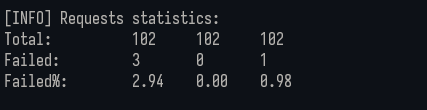
\includegraphics[width=0.65\textwidth]{screenshots/test-network-comm}
    \caption{\label{img:test-network-comm}Zrzut ekranu z~monitora portu szeregowego podczas testowania komunikacji
        w~sieci.}
\end{figure}

\FloatBarrier
\section{\label{sect:test-webserver-comm}Testy transmisji danych do serwera sieciowego} Wykonane zostały także testy
komunikacji modułu MASTER z~modułem serwera sieciowego. Sprawdzone zostało czy dane zbierane przez sieć LoRa poprawnie
przesyłane przez magistralę I2C oraz dekodowane po stronie modułu serwera sieciowego.

Korzystając z~zaimplementowanego logowania przez port szeregowy modułu MASTER informacji o~transmisji przez magistralę
I2C (listing \ref{lst:main-transmitting}) oraz dodatkowej funkcjonalności w~module serwera sieciowego, której
implementacja przedstawiona została na listingu \ref{lst:webserver-count-transmission}, logującej przez port szeregowy
ilość odebranych transmisji, sprawdzona została poprawność komunikacji.

\lstinputlisting[
    language=c++,
    linerange={129-135},
    caption={Implementacja funkcjonalności zliczania transmisji z~modułu MASTER na module serwera sieciowego.},
    label={lst:webserver-count-transmission},
    float=htbp
]{feather-ws/src/main.cpp}

Moduły zostały uruchomione oraz włączony został monitor portu szeregowego modułu MASTER oraz modułu serwera sieciowego.
Przez pewien czas prowadzona była obserwacja logowanych wartości. Podczas trwania testu stwierdzone zostało, że moduły
działają i~komunikują się poprawnie. Przykładowe logi, pokazujące poprawną komunikację przedstawione zostały na rys.
\ref{img:test-i2c-master} oraz \ref{img:test-i2c-webserver}.

\begin{figure}[!htbp]
    \centering
    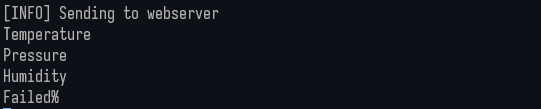
\includegraphics[width=0.70\textwidth]{screenshots/test-i2c-master}
    \caption{\label{img:test-i2c-master}Logi o~transmisji przez magistralę I2C z~modułu MASTER.}
\end{figure}

\begin{figure}[!htbp]
    \centering
    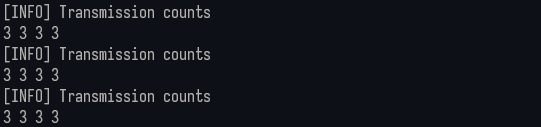
\includegraphics[width=0.70\textwidth]{screenshots/test-i2c-webserver}
    \caption{\label{img:test-i2c-webserver}Logi pokazujące poprawne odbieranie wartości z~magistrali I2C przez moduł
        serwera sieciowego.}
\end{figure}

\FloatBarrier
\section{\label{sect:test-webserver-website}Testy działania serwera seciowego oraz strony internetowej} Ostatnim
wykonanym testem, który pozwolił na stwierdzenie, że zaimplementowane oprogramowanie działa poprawnie było sprawdzenie
samego serwera sieciowego. Zweryfikowane zostało czy uruchamia się on poprawnie, gdy pojawi się możliwość zalogowania do
sieci lokalnej sieci WiFi (której dane zostały podane w~pliku konfiguracyjnym) oraz czy poprawnie działa strona
internetowa, którą moduł serwuje użytkownikowi, chcącemu zobaczyć zebrane przez sieć LoRa dane.

Do testu wykorzystany został mobilny hotspot (lokalna sieć WiFi utworzona przez smartphone) oraz zaimplementowana
rejestracja informacji o~logowaniu się modułu do sieci WiFi i~uruchamiania serwera sieciowego. Na rys.
\ref{img:wifi-hotspot} oraz \ref{img:webserver-wifi-logging} pokazana została włączony mobilny hotspot oraz logi
z~modułu serwera sieciowego. Na ich podstawie stwierdzone zostało, że serwer sieciowy działa poprawnie, ponieważ jednym
z~logów jest informacja o~starcie serwera z~jego lokalnym IP (umożliwającym wyświetlenie strony internetowej) na porcie
80.

\begin{figure}[!htbp]
    \centering
    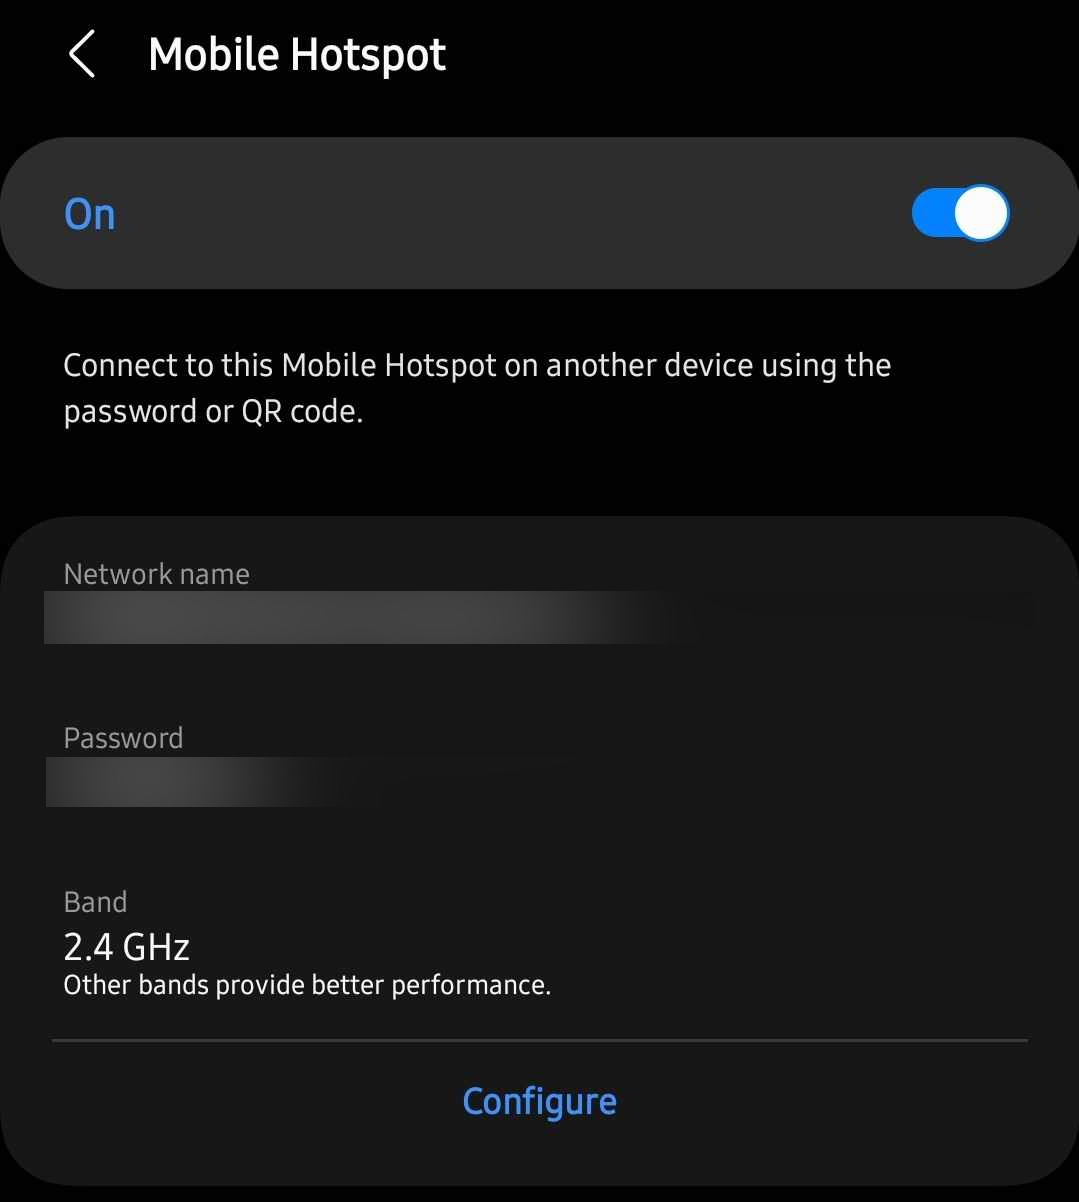
\includegraphics[width=0.50\textwidth]{screenshots/wifi-hotspot}
    \caption{\label{img:wifi-hotspot}Zrzut ekranu pokazujący włączony mobilny hotspot.}
\end{figure}

\begin{figure}[!htbp]
    \centering
    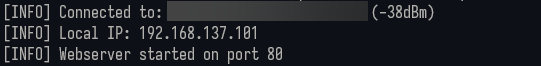
\includegraphics[width=0.70\textwidth]{screenshots/webserver-wifi-logging}
    \caption{\label{img:webserver-wifi-logging}Logi pokazujące poprawne połączenie z~siecią WiFi oraz uruchomienie
        serwera sieciowego.}
\end{figure}

\FloatBarrier
Działanie zaimplementowanej strony internetowej sprawdzone zostało poprzez wykonanie próby załadowania jej w~dwóch
przypadkach: przed pierwszym przesłaniem danych z~sieci LoRa (lub tuż po restarcie modułu serwera sieciowego) oraz po
tym jak dane zostały przesłane. Miało to na celu sprawdzenie, poza samym ładowaniem strony, także czy jej zawartość
zostanie poprawnie zaktualizowana, gdy z~modułu MASTER przesłane zostaną dane. Rys. \ref{img:website-pre-data} pokazuje
poprawnie załadowaną stronę przed przesłaniem danych z~sieci LoRa, natomiast rys. \ref{img:website-post-data} to zrzut
ekranu z~widoczoną poprawną aktualizacją danych po odebraniu ich przez moduł serwera sieciowego.

\begin{figure}[!htbp]
    \centering
    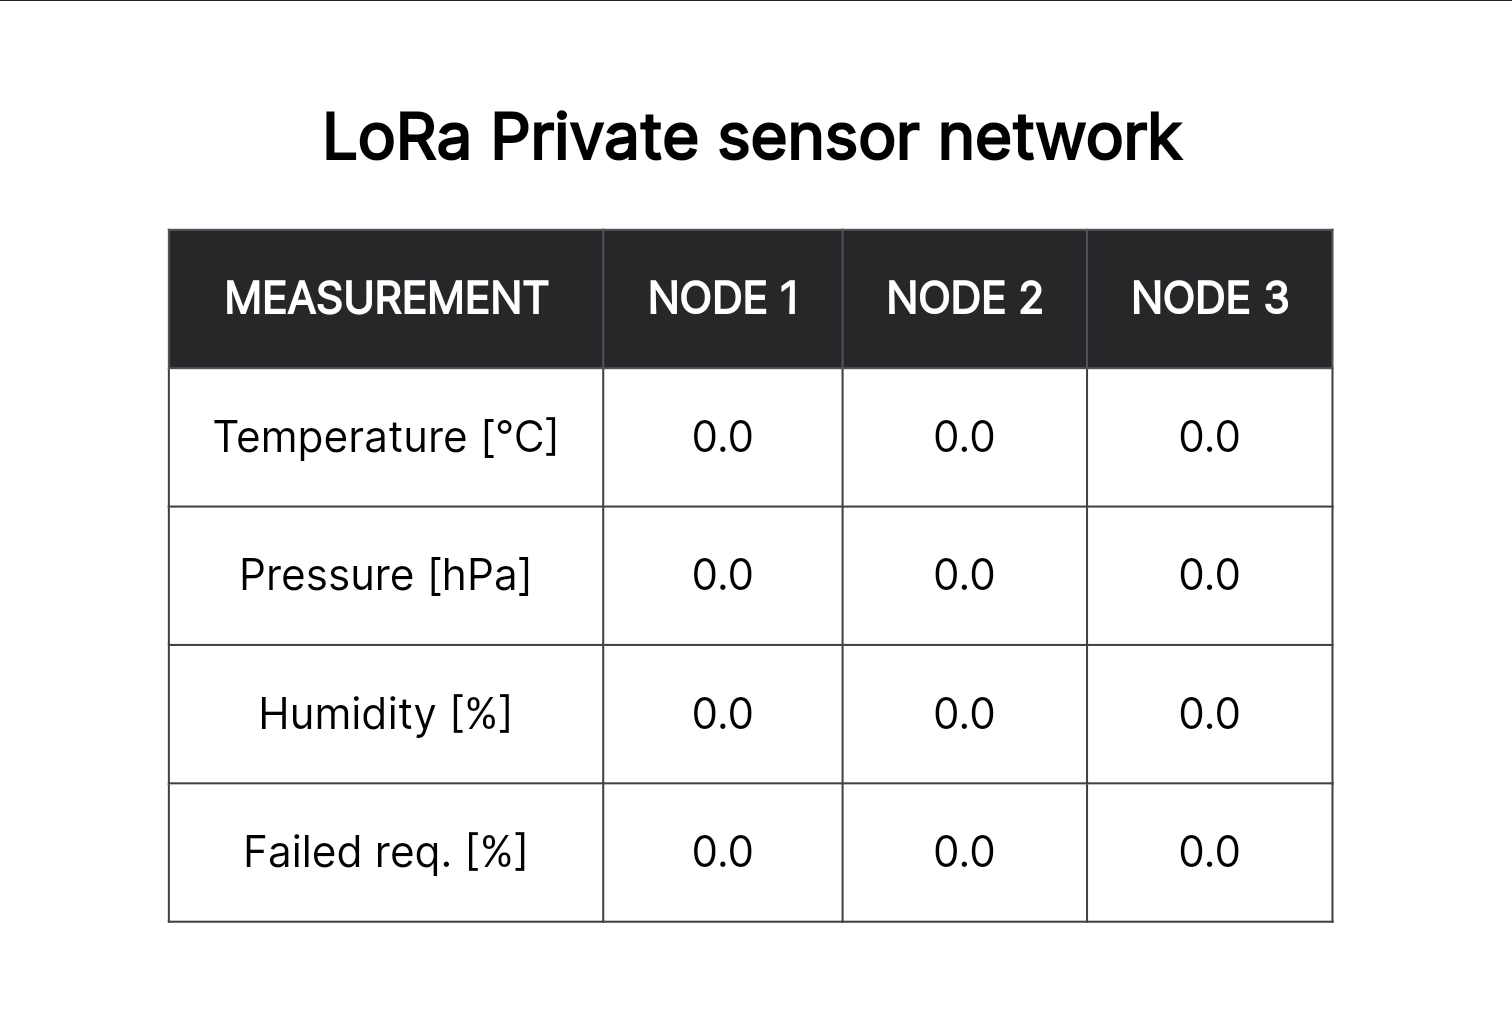
\includegraphics[width=0.65\textwidth]{screenshots/website-pre-data}
    \caption{\label{img:website-pre-data}Zrzut ekranu ze strony bez danych z~sieci.}
\end{figure}

\begin{figure}[!htbp]
    \centering
    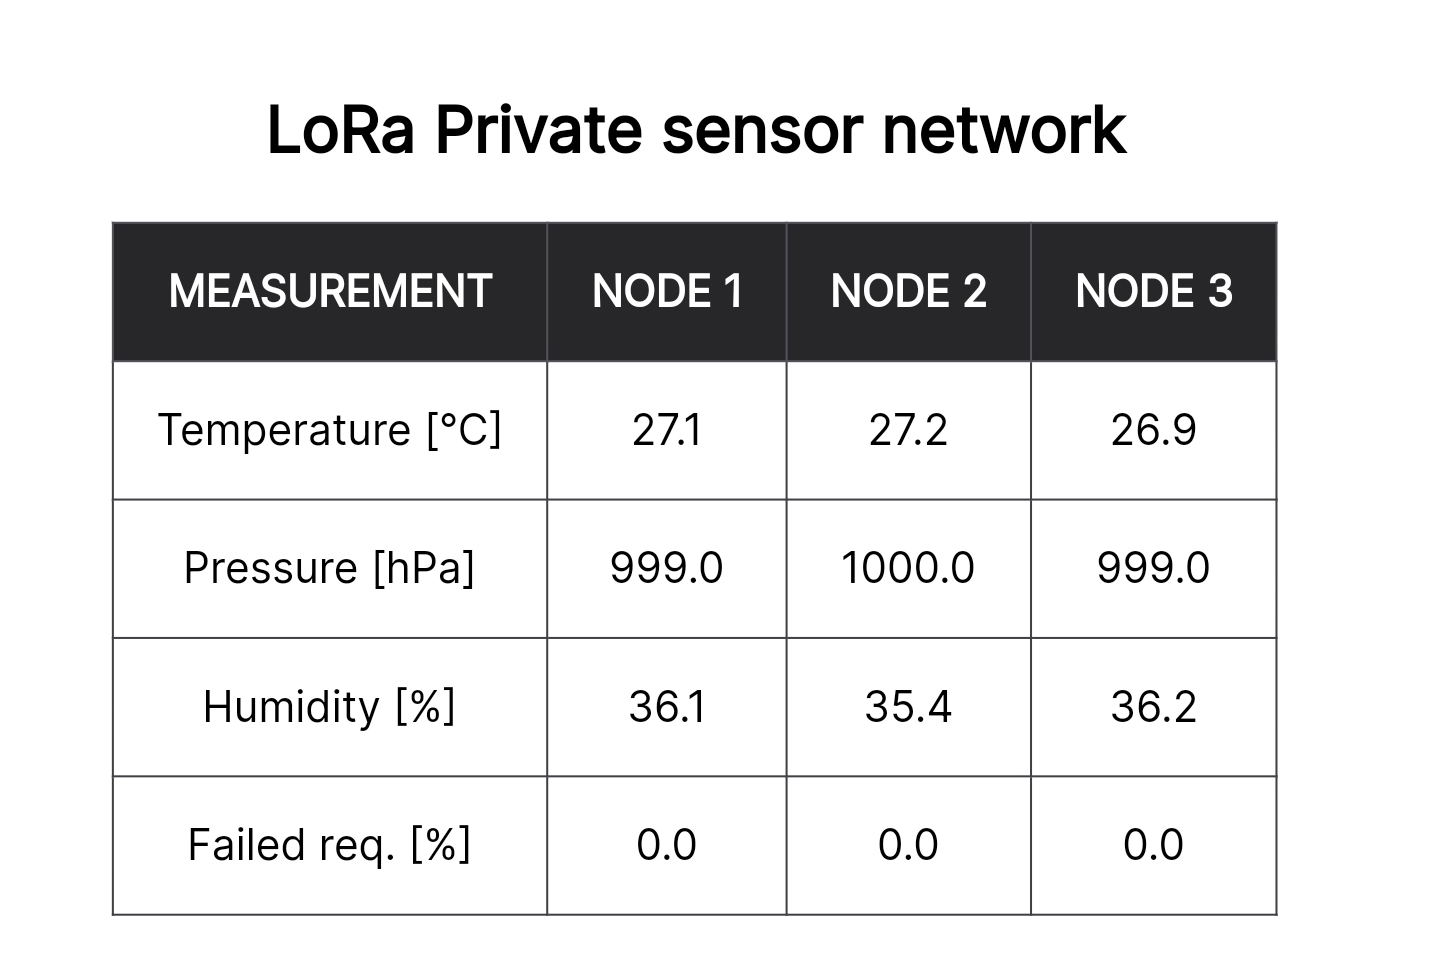
\includegraphics[width=0.65\textwidth]{screenshots/website-post-data}
    \caption{\label{img:website-post-data}Zrzut ekranu ze strony po otrzymaniu danych przez moduł serwera sieciowego.}
\end{figure}


\chapter{\label{ch:research}Badania działającej sieci}
W~celu określenia czy możliwe jest zbudowanie funkcjonalnej, prywatnej sieci czujnikowej opierając się o~standard LoRa,
przeprowadzony został zestaw badań. Pozwoliły one na dokładniejsze zapoznanie się ze standardem oraz jego możliwościami.
Zbadane zostały elementy podstawowe -- jakość komunikacji pomiędzy modułami, w~celu określenia czy wykorzystanie takiej
sieci nie wiąże się z~większymi problemami niż typowe standardy jak np. ZigBee. Zbadane zostały też parametry sieci
podczas jej pracy -- zasięg komunikacji, zużycie energii. Przeprowadzona została także analiza widmowa, w~celu
zaobserwowania jak wygląda komunikacja w~standardzie LoRa -- celem tego badania była próba zaobserwowania oraz analizy
techniki, jaką standard wykorzystuje do transmisji danych -- tzw. Chirp.

\section{\label{sect:network-comm}Badanie komunikacji w~sieci} Podstawowym badaniem było sprawdzenie poprawności
komunikacji w~dłuższym okresie niż kilka minut. Miało ono na celu określenie czy wybór standardu LoRa jest wyborem
dobrym do prób implementacji sieci czujnikowej. Badanie to było rozszerzeniem testu implementacji, które pozwoliło na
sprawdzenie jakości komunikacji. W~przypadku, gdyby wynik badania pokazał, że sieć ma problemy z~komunikacją, który nie
było widać w~krótkich testach, należałoby przemyśleć czy standard LoRa jest poprawnym wyborem.

Aby otrzymać zestaw danych testowych, moduły pozostały włączone, bez restartowania ich, przez 1~godzinę. Przy ustawieniu
okresu pomiędzy wysyłaniem żądań przez moduł MASTER na 1~minutę dało to 61 pełnych wymian danych w~sieci -- 1~żądanie
przy pierwszym uruchomieniu modułu MASTER oraz 60 podczas pracy modułu na zaimplementowanym zegarze (w sumie 183 żądania
do każdego modułu SLAVE). Średnia odległość pomiędzy modułami podczas badania wynosiła 0.45m (45cm).

\begin{table}[!htbp]
    \centering
    \caption{\label{tab:1h-comm-test}Wyniki przeprowadzonego badania komunikacji w~czasie 1~godziny.}
    \begin{tabular}{@{}lccc@{}}
        \toprule
        Zapytania         & \multicolumn{1}{l}{SLAVE 1} & \multicolumn{1}{l}{SLAVE 2} & \multicolumn{1}{l}{SLAVE 3} \\ \midrule
        W~sumie {[}-{]}   & 183                         & 183                         & 183                         \\
        Nieudane {[}-{]}  & 4                           & 0                           & 1                           \\
        Nieudane {[}\%{]} & 2.19                        & 0                           & 0.55                        \\ \bottomrule
    \end{tabular}
\end{table}

\FloatBarrier
Na podstawie zebranych danych sporządzony został wykres, przedstawiający otrzymane wyniki  -- sumę wysłanych zapytań
oraz ilość, która zakończyła się błędem. Przedstawiony on został na rysunku \ref{img:network-communication-1h}. Kolorem
niebieskim oznaczono sumę wysłanych zapytań, natomiast kolorem pomarańczowym ilość z~brakiem odpowiedzi lub odrzucone
z~powodu błędu. Korzystając z~zebranych danych, możliwe jest zaobserwowanie, że podczas dłuższej komunikacji jedynie
niewielki procent zapytań kończy się błędem, a~wykorzystanie standardu LoRa jest wyborem, pozwalającym na budowanie
sieci czujnikowych.

\begin{figure}[!htbp]
    \centering
    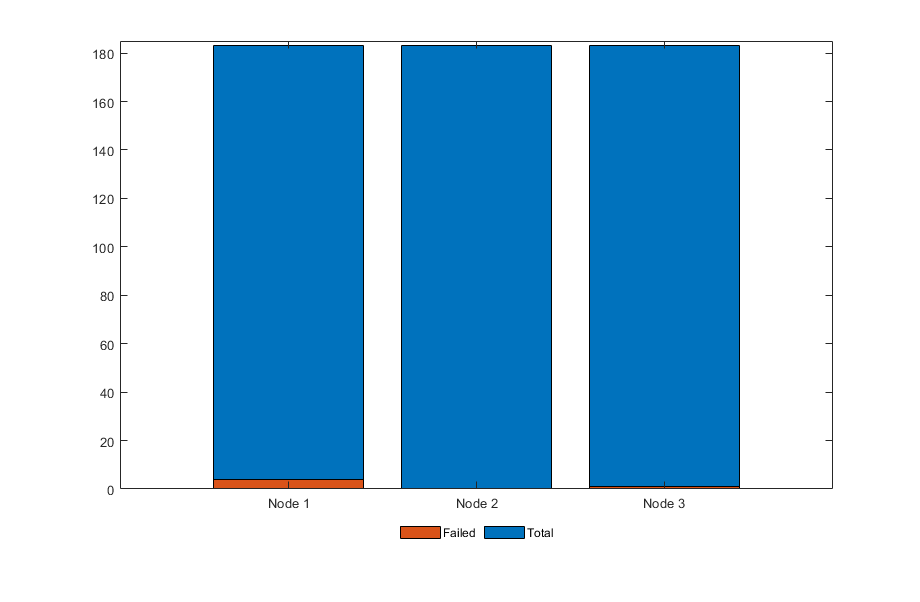
\includegraphics[width=0.8\textwidth]{research/network-communication-1h}
    \caption{\label{img:network-communication-1h}Wykres słupkowy przedstawiający wyniki 1-godzinnego testu komunikacji
        sieci}
\end{figure}

\FloatBarrier
\section{\label{sect:spectral-analisys}Analiza widmowa transmisji w~standardzie LoRa} Aby dokładniej zapoznać się z~tym,
jak działa komunikacja w~standardzie LoRa, wykonana została analiza widmowa transmisji pomiędzy modułami sieci.
Wykorzystane tutaj zostało narzędzie pozwalające na badanie fal radiowych bazujące na SDR (ang. \textsl{Software Defined
    Radio}) -- Hack RF One oraz darmowe, udostępnione w~charterze open source, oprogramowanie \textsl{gqrx} na platformę
Linux. Celem tego badania była obserwacja spektrum sygnałów radiowych w~okolicach częstotliwości, na jakich operuje
LoRa, oraz próba zaobserwowania czy możliwe jest metodą tą zobaczenie pojedynczych chirpów podczas transmisji.
Stanowisko testowe zostało wykorzystane także do zebrania zestawu próbek I/Q, które, w~późniejszym czasie, zostały
poddane analizie wykorzystując do tego środowisko MATLAB.

\subsection{\label{sect:spectral-in-gqrx}Obserwacje transmisji w~oprogramowaniu \textsl{gqrx}} Moduły zostały ustawione
na stanowisku testowym, odległość pomiędzy nimi podczas badania wynosiła, podobnie jak w~przypadku badania komunikacji,
około 0.45m. W~odległości około 1m od ustawionej sieci znajdowała się antena podłączona do Hack RF One. Oprogramowanie
\textsl{gqrx} ustawione zostało w~taki sposób, aby móc odczytywać w~nim dane zbierane przez urządzenie -- rozmiar okna
FFT na 1048576 próbek (maksymalna wartość dostępna w~programie), co dawało rozdzielczość pasma przenoszenia 1Hz oraz
częstotliwość odświeżania na 60fps (ang. \textsl{frames per second} -- klatek na sekundę, maksymalna dostępna). Na tak
przygotowanym stanowisku testowym uruchomione zostały moduły. Aby uzyskać lepszą dokładność obserwacji, na modułach
wyłączona została funkcjonalność pracy na zegarze, a~transmisja uruchamiana była każdorazowo ręcznie (wykorzystując
przycisk na module MASTER).

Pierwsze próby obserwacji komunikacji przeprowadzone zostały na podstawowych ustawieniach modułów -- najniższa wartość
Spreading Factor, SF7 (7 bitów na symbol), pasmo 125kHz, radio coding rate, CR, 4/5. Takie parametry pozwalają sieci na
szybką komunikację, jednakże w~przypadku analizy widmowej nie pozwoliły one na dobrą obserwację transmisji. W~tym celu
parametr Spreading Factor przestawiony został na wartość maksymalną, SF12 (12 bitów na symbol). Spowodowało to
wydłużenie czasu każdej transmisji i~jednocześnie pozwoliło na lepszą obserwację. Korzystając ze zmodyfikowanych
parametrów, wykonane zostało kilkanaście transmisji i~w tym czasie obserwowane było, jak wygląda ich widmo. Rys.
\ref{img:waterfall-full-mid-transmission} przedstawione zostało, jak wyglądała obserwowana transmisja (tutaj: pełna sieć,
w~trakcie transmisji przez jeden z~modułów).

\begin{figure}[!htbp]
    \centering
    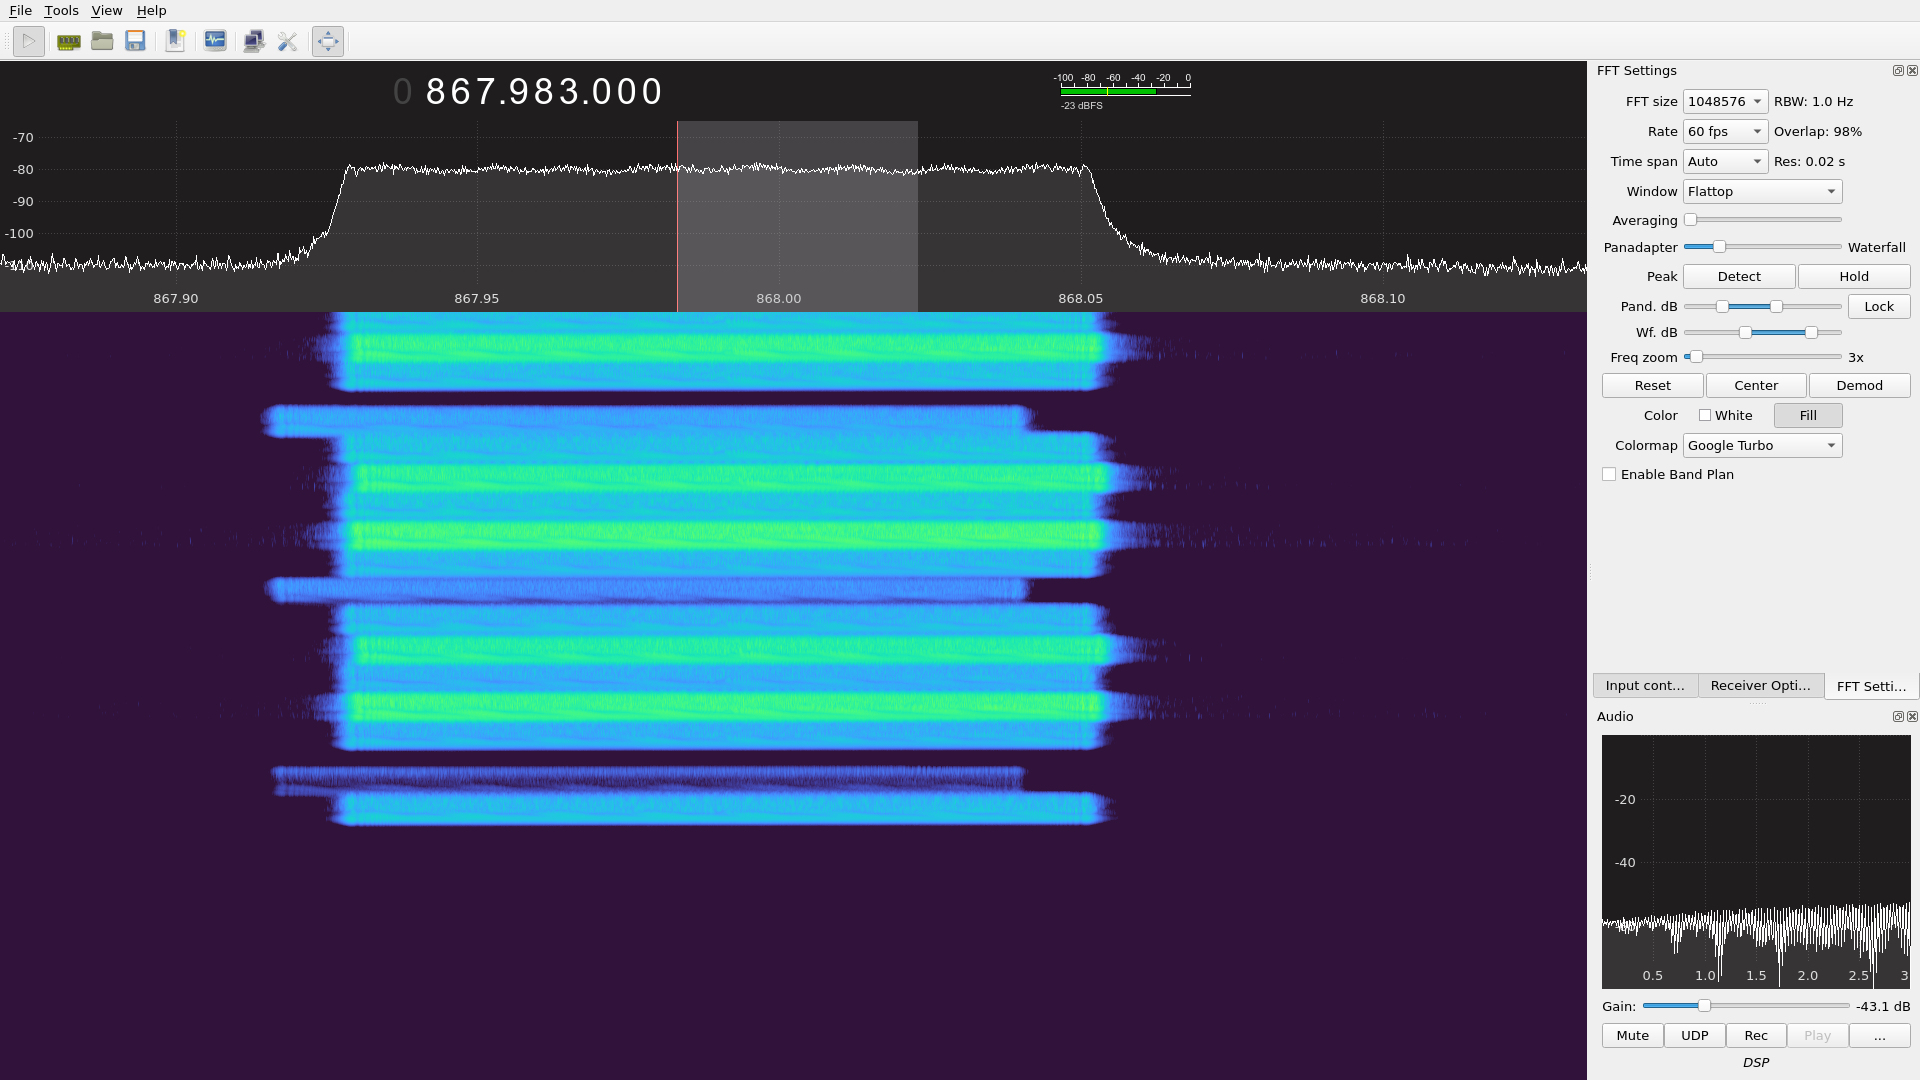
\includegraphics[width=0.9\textwidth]{research/waterfall-full-mid-transmission}
    \caption{\label{img:waterfall-full-mid-transmission}Zrzut ekranu z~programu pokazujący obserwowane transmisje}
\end{figure}

\FloatBarrier
Podczas badania wykonane zostały transmisje w~kilku konfiguracjach -- pełna sieć, 2~moduły SLAVE oraz 1~moduł SLAVE.
W~tym czasie wykonywane zostały zrzuty ekranów widoku z~programu \textsl{gqrx}. Na rys.
\ref{img:waterfall-full-no-timeouts}, \ref{img:waterfall-full-with-timeouts}, \ref{img:waterfall-one-slave} oraz
\ref{img:waterfall-two-slave} przestawione zostały wyniki obserwacji.

\begin{figure}[!htbp]
    \centering
    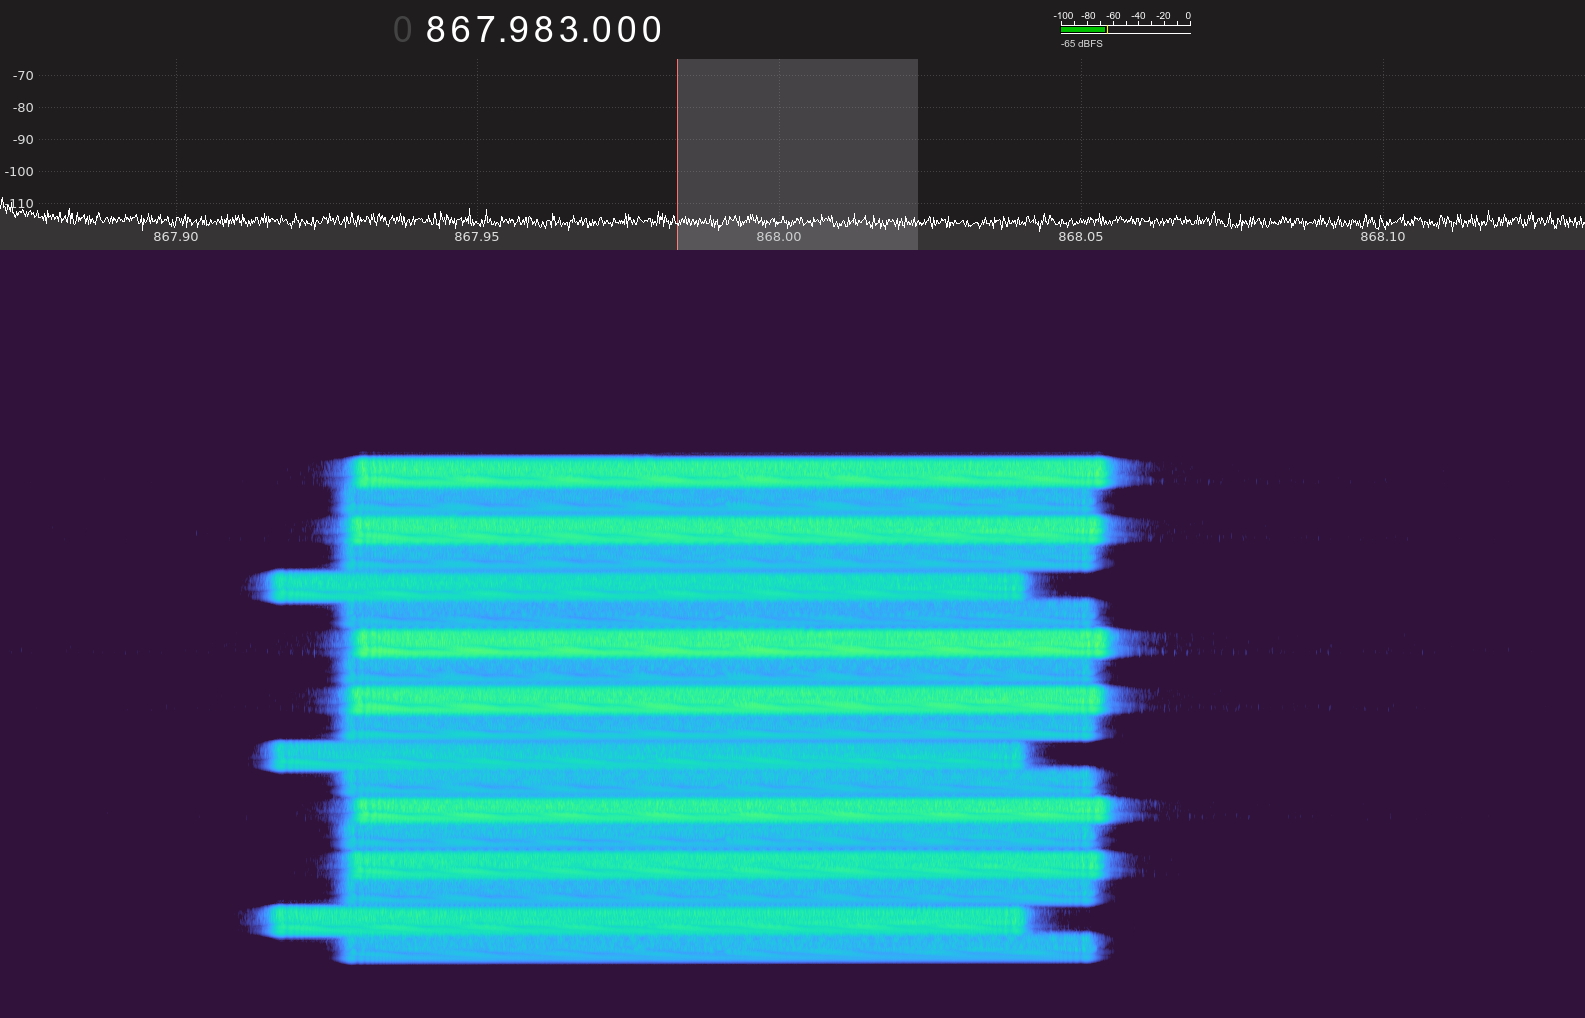
\includegraphics[width=0.9\textwidth]{research/waterfall-full-network-no-timeouts}
    \caption{\label{img:waterfall-full-no-timeouts}Widok na komunikację pełnej sieci, bez wystąpienia problemów
        z~komunikacją}
\end{figure}

\begin{figure}[!htbp]
    \centering
    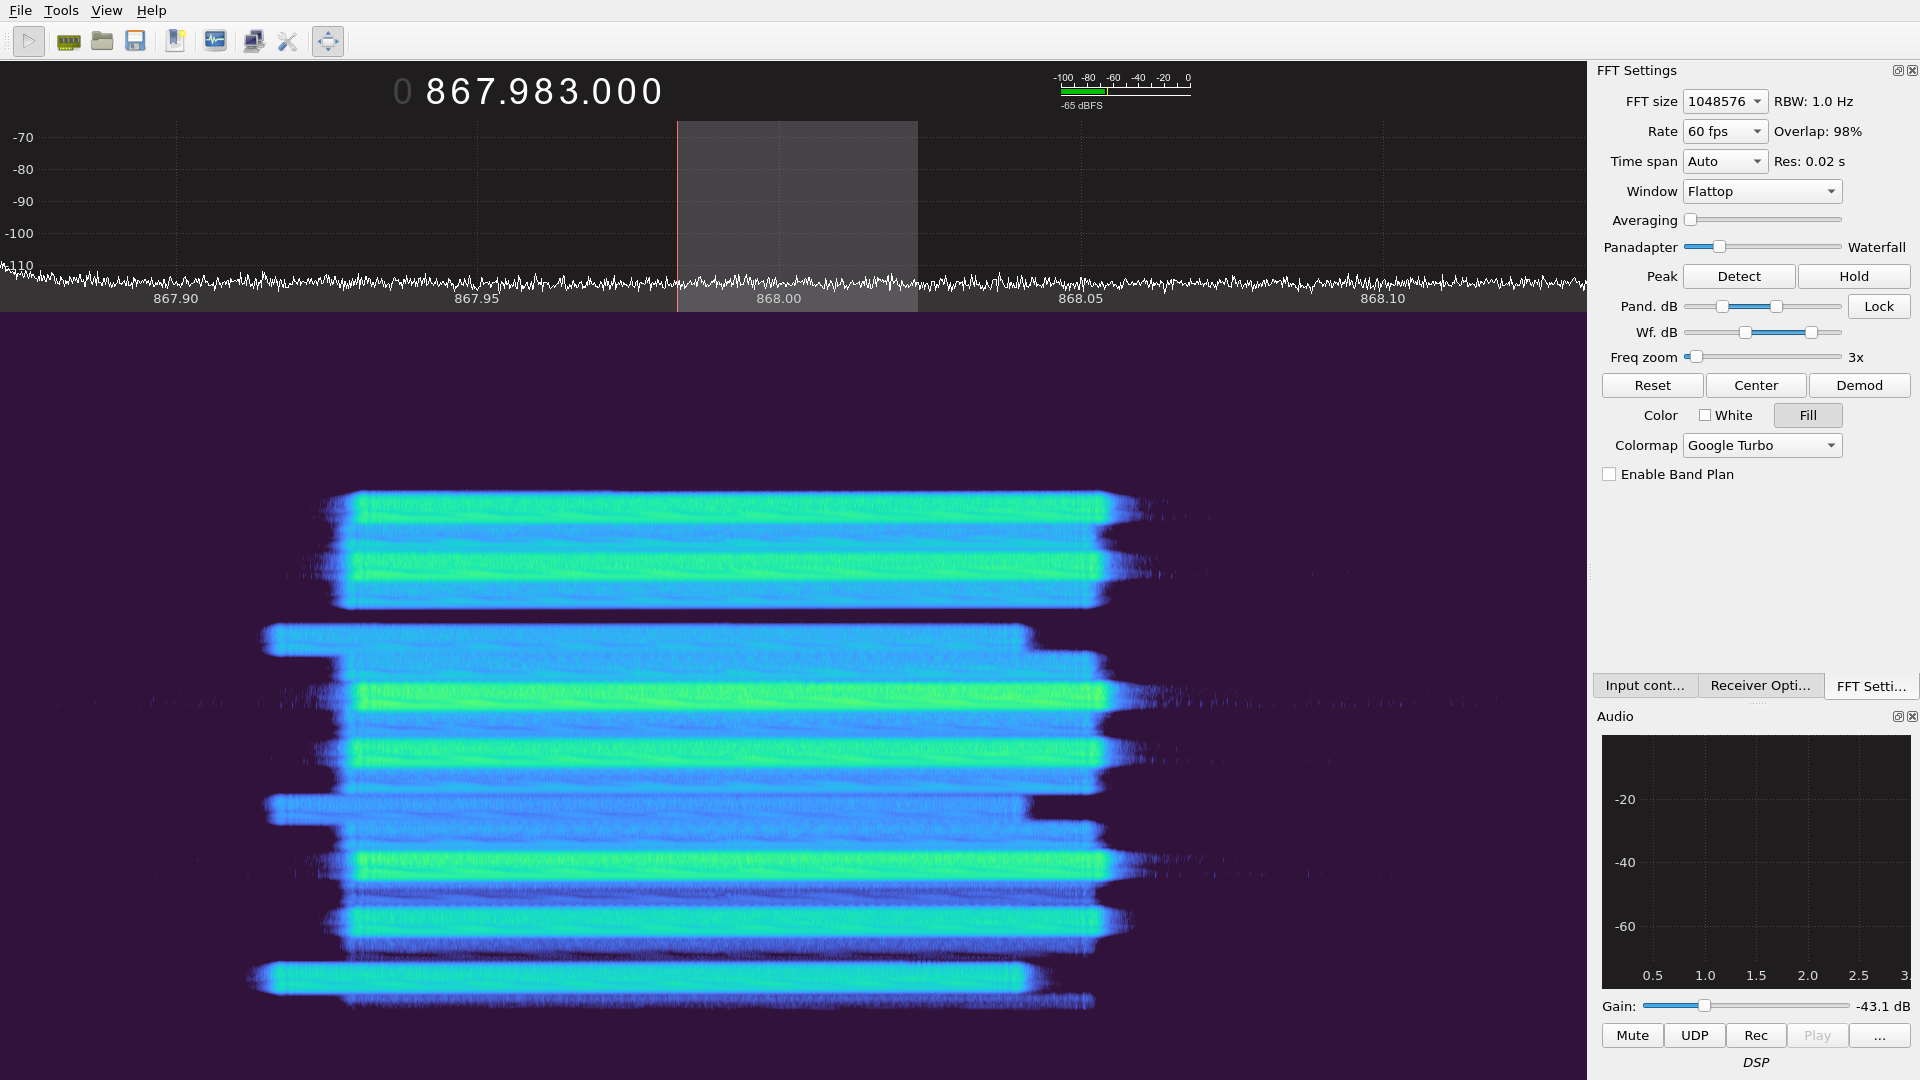
\includegraphics[width=0.9\textwidth]{research/waterfall-full-network-with-timeouts}
    \caption{\label{img:waterfall-full-with-timeouts}Widok na komunikację pełnej sieci, z~widocznymi przerwami, gdy
        jeden z~modułów nie odpowiedział na zapytanie}
\end{figure}

\begin{figure}[!htbp]
    \centering
    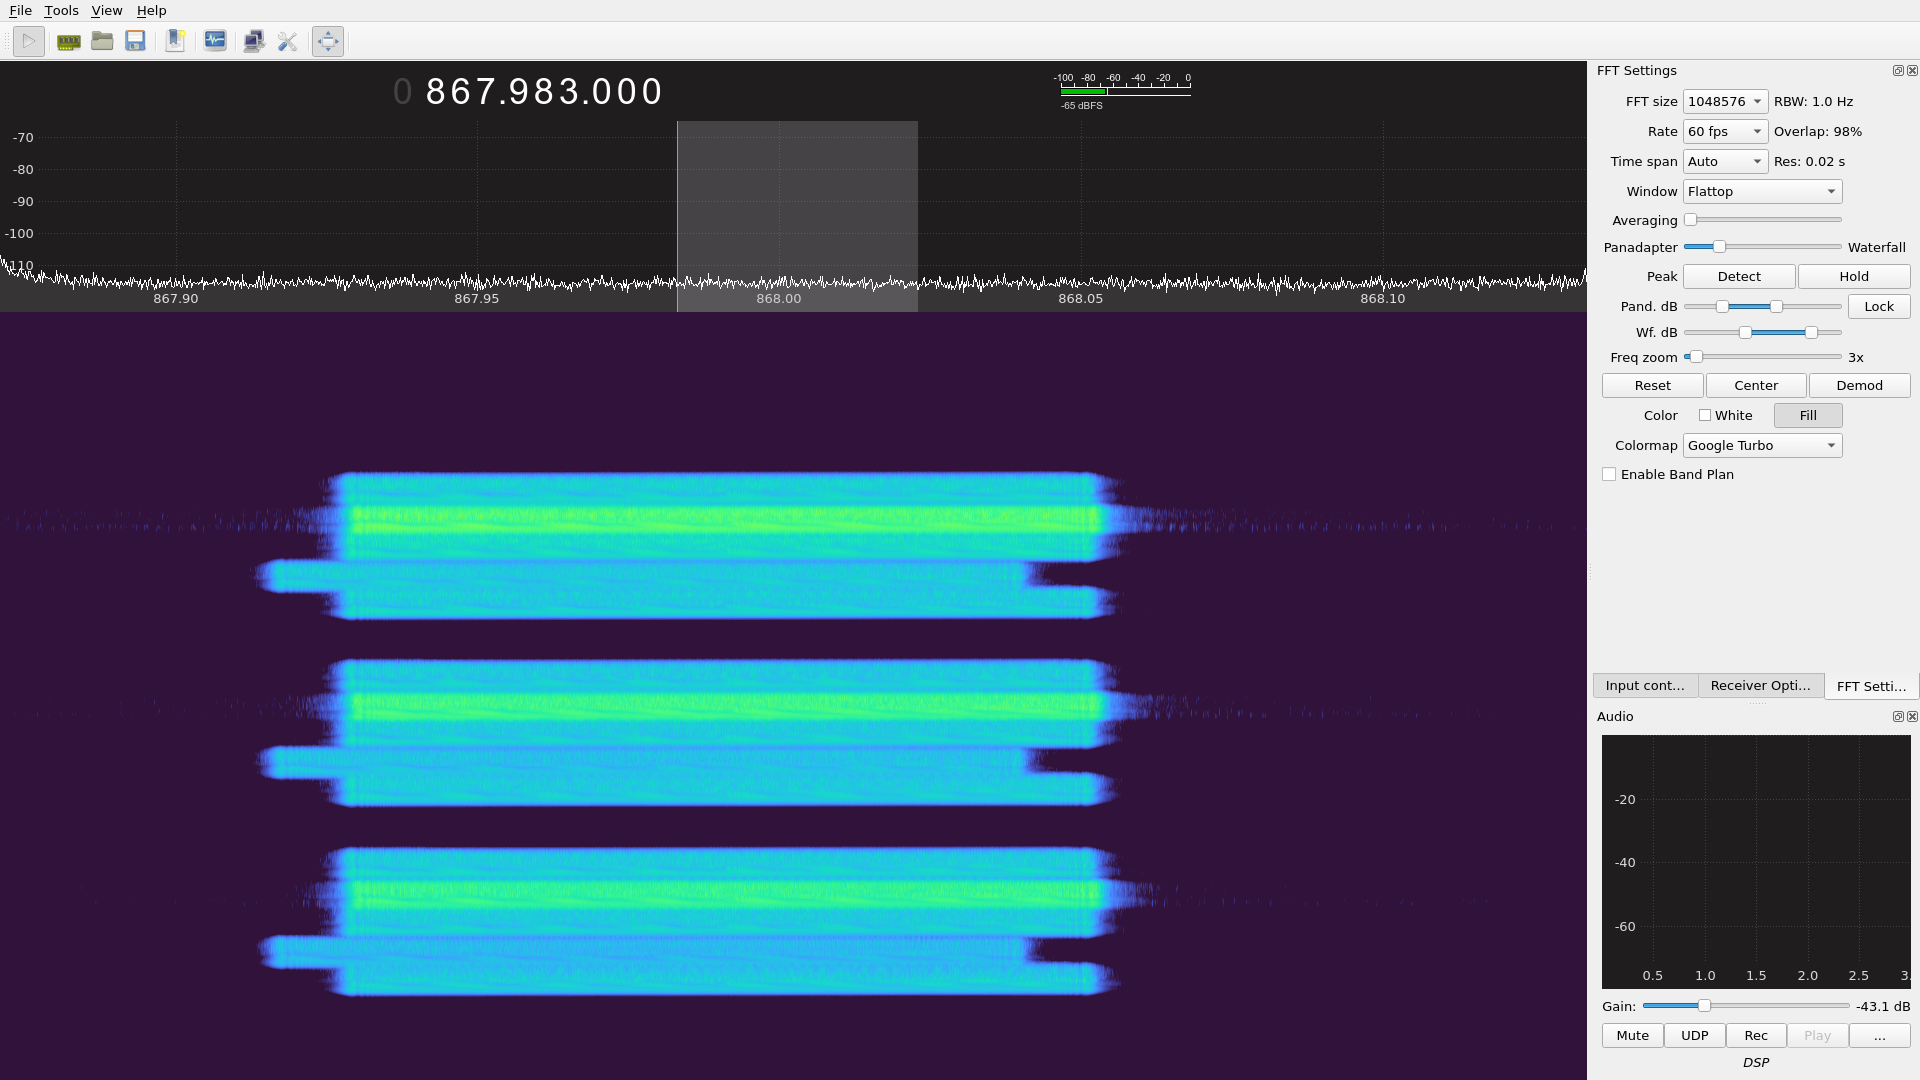
\includegraphics[width=0.9\textwidth]{research/waterfall-two-slave-network}
    \caption{\label{img:waterfall-one-slave}Widok na komunikację w~sieci dwoma modułami SLAVE włączonymi, a~jednym
        wyłączonym}
\end{figure}

\begin{figure}[!htbp]
    \centering
    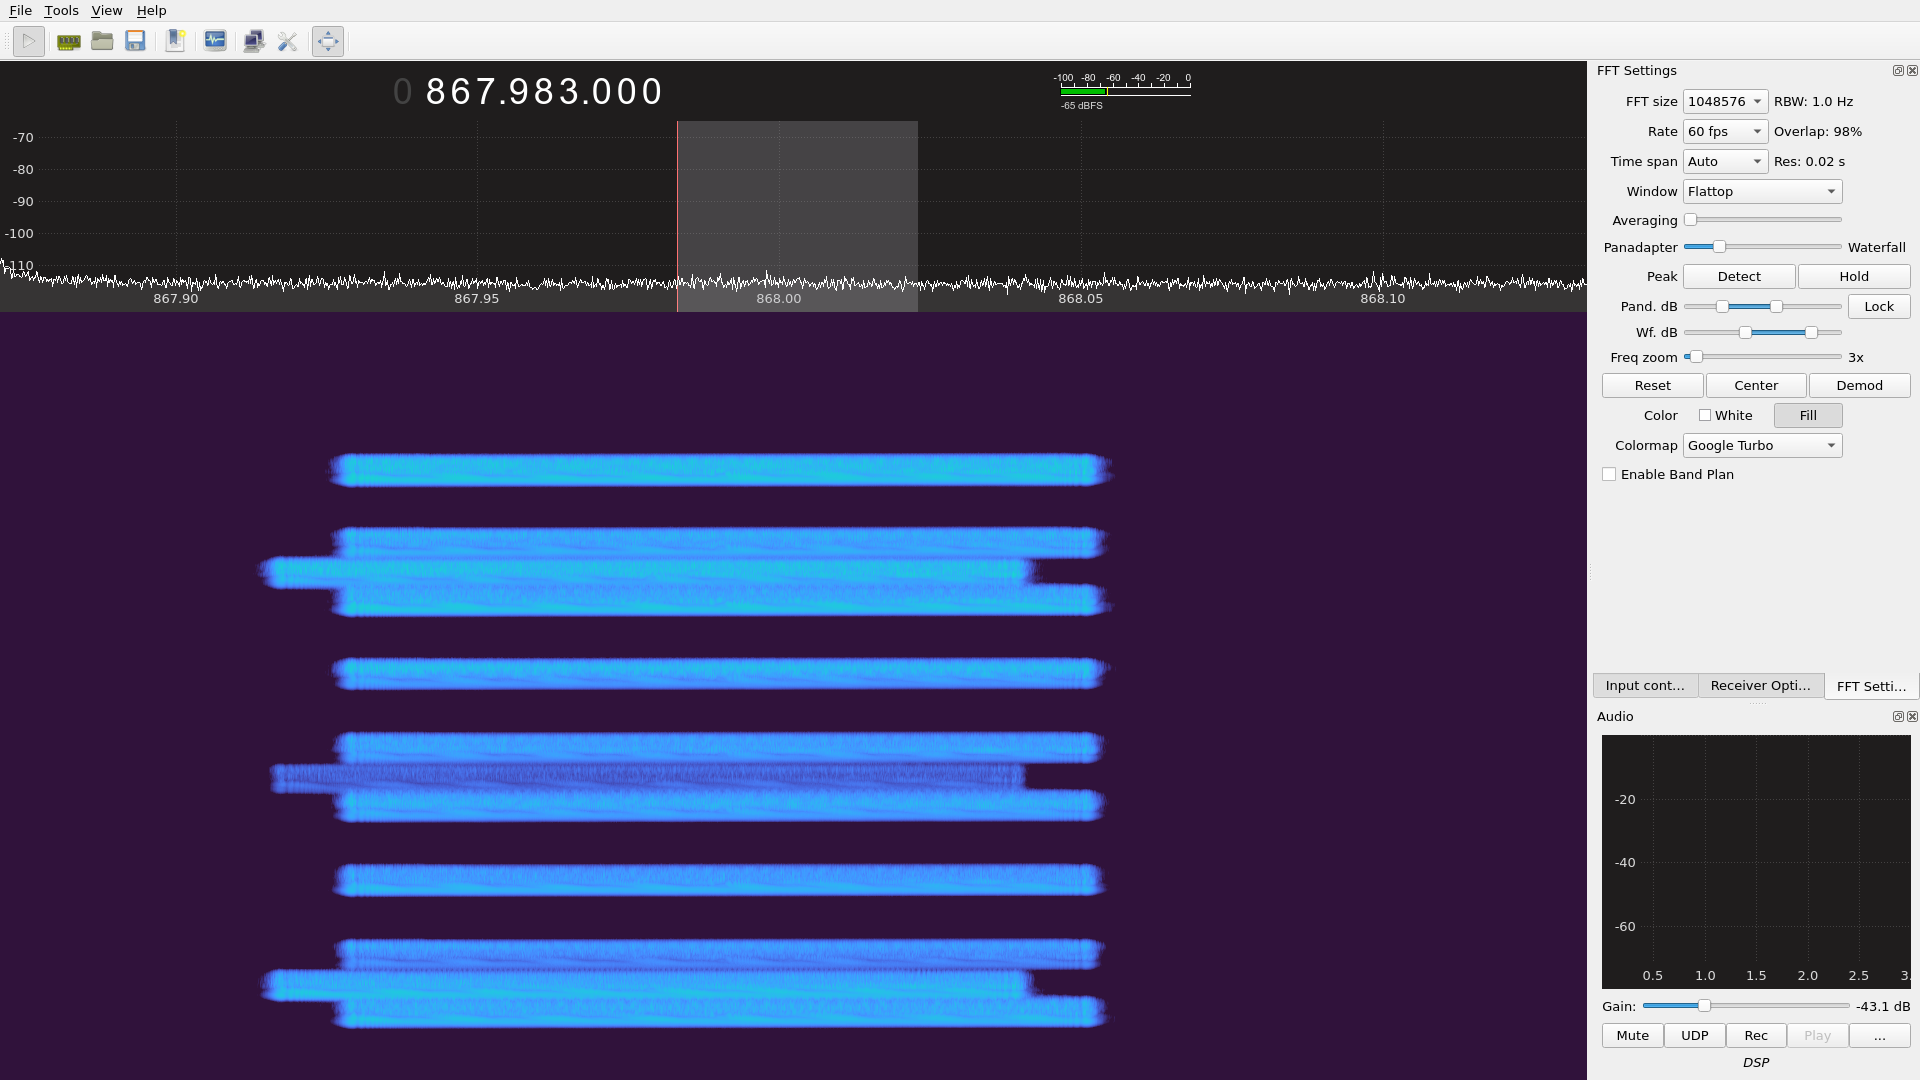
\includegraphics[width=0.9\textwidth]{research/waterfall-one-slave-network}
    \caption{\label{img:waterfall-two-slave}Widok na komunikację w~sieci z~tylko jednym modułem SLAVE włączonymi}
\end{figure}

\FloatBarrier
W~przypadku, gdzie udało się zaobserwować pełną komunikację, gdzie nie wystąpiły żadne problemy, wyraźnie widać 9~wymian
pomiędzy modułami (18 transmisji). Natomiast w~przypadkach, gdy pojawił się błąd, bądź dany moduł był wyłączony wyraźnie
widać to w~zaobserwowanym zapisie. Niestety w~przypadku obserwacji wykorzystując do tego program \textsl{gqrx} nie udało
zaobserwować się pojedynczych elementów każdej transmisji (pojedynczych chirpów, preambuły czy wysyłanych symboli). Jest
to związane z~ograniczeniami oprogramowania co do maksymalnej szybkości odświeżania widoku na ekranie.

Poza obserwacją tzw. wykresów wodospadowych (pokazujących zmiany w~widmie w~czasie) udało się także zebrać zapisy
rozkładu częstotliwości sygnałów podczas transmisji wykonywanych przez moduły. Przedstawione zostało to na rys.
\ref{img:frequency-graph-no-transmission}, \ref{img:frequency-graph-master-request} oraz
\ref{img:frequency-graph-slave-response}. Ciekawym faktem jest tutaj widoczna w~przypadku transmisji z~modułów SLAVE
wyższa moc sygnałów. Spowodowane to było najprawdopodobniej faktem, że były umieszczone bliżej anteny podłączonej do
urządzenia zbierającego dane.

\begin{figure}[!htbp]
    \centering
    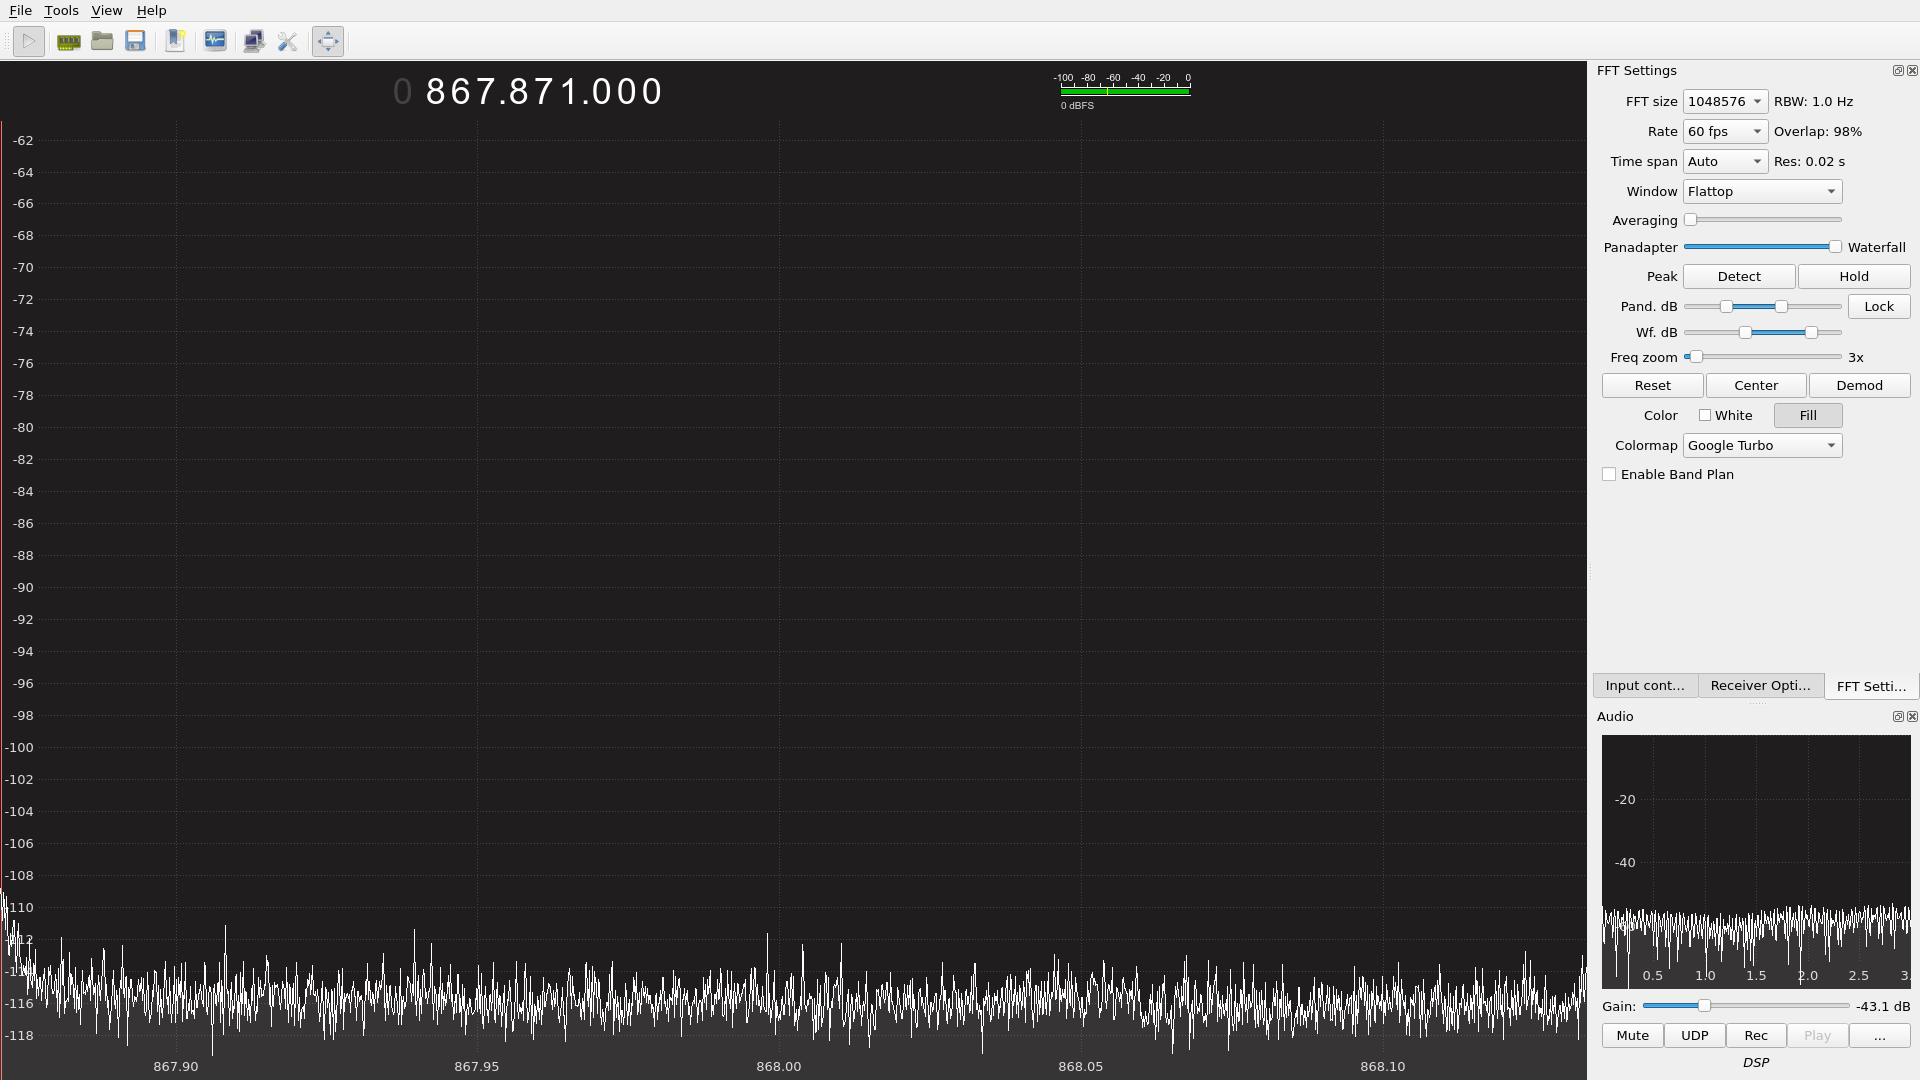
\includegraphics[width=0.9\textwidth]{research/frequency-graph-no-transmission}
    \caption{\label{img:frequency-graph-no-transmission}Widok spektrum częstotliwości, gdy żaden z~modułów nie transmituje}
\end{figure}

\begin{figure}[!htbp]
    \centering
    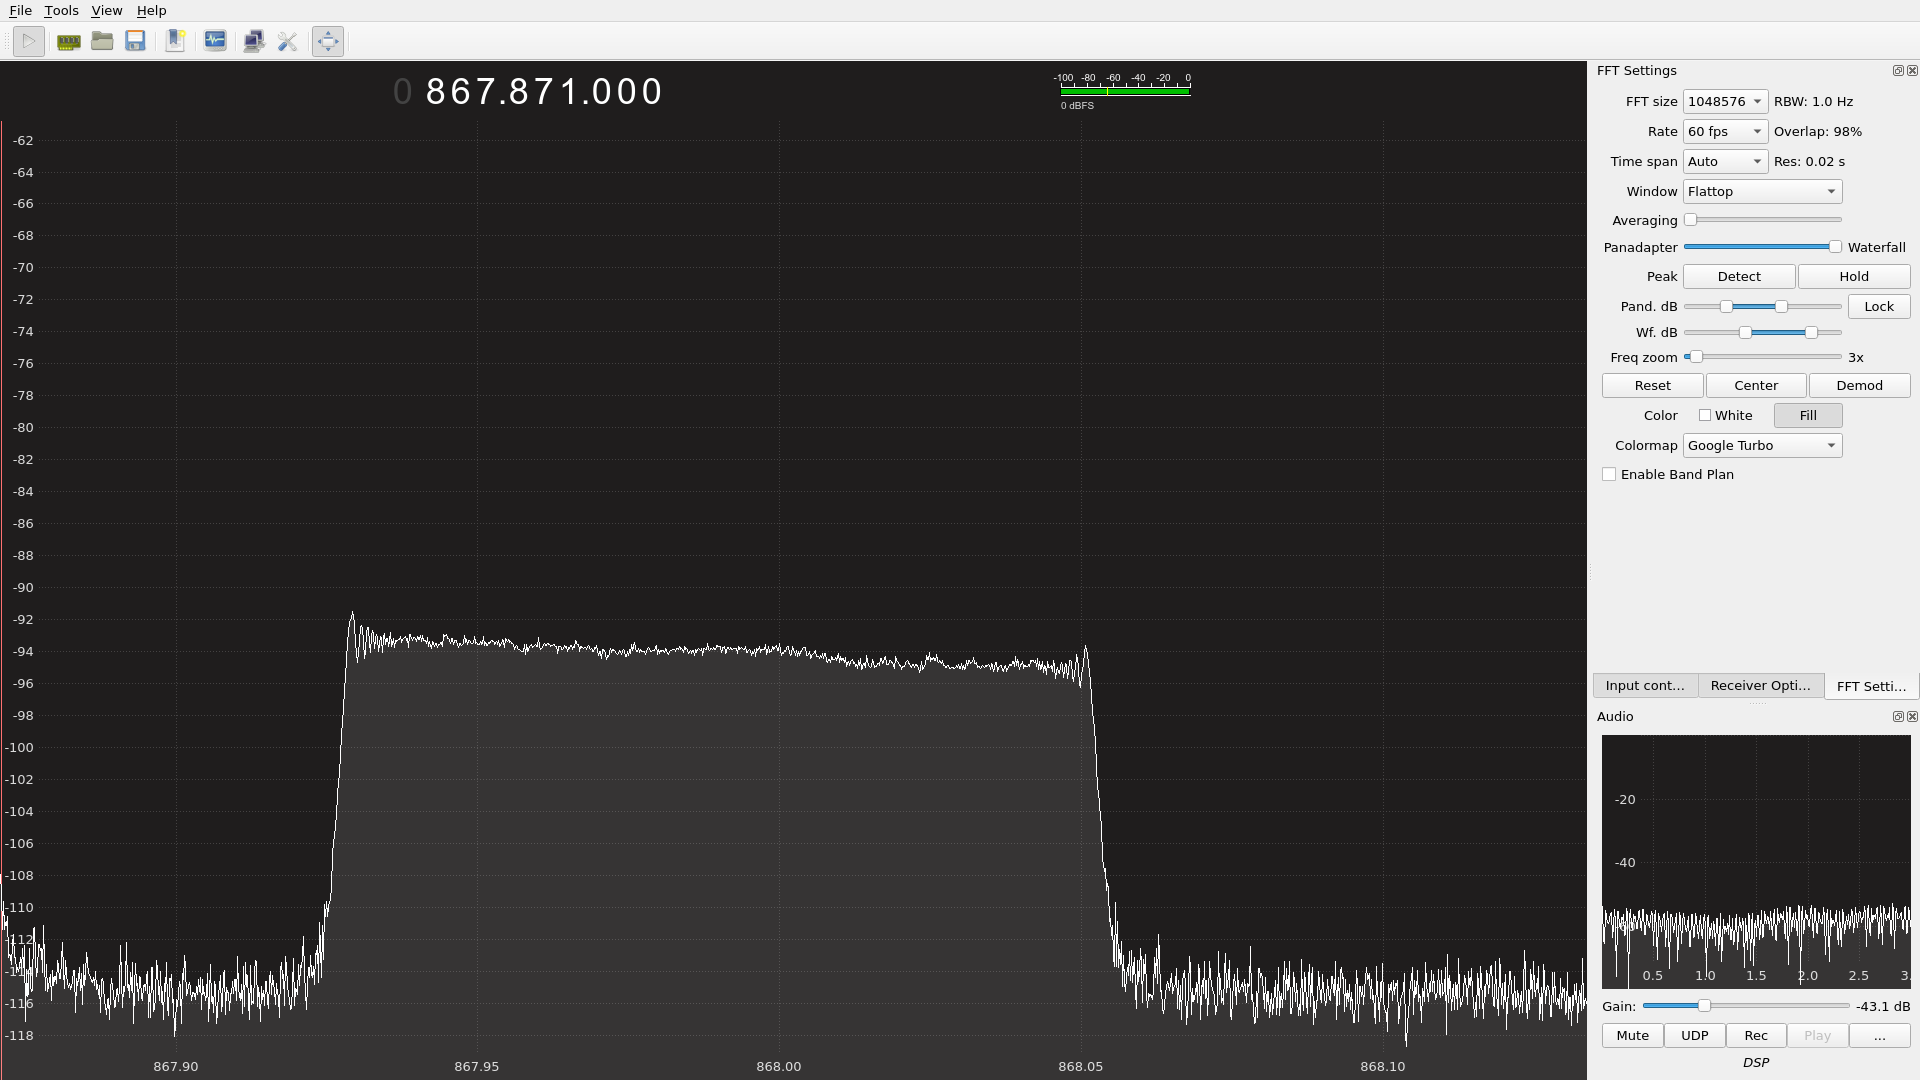
\includegraphics[width=0.9\textwidth]{research/frequency-graph-master-request}
    \caption{\label{img:frequency-graph-master-request}Widok spektrum częstotliwości podczas transmisji modułu MASTER}
\end{figure}

\begin{figure}[!htbp]
    \centering
    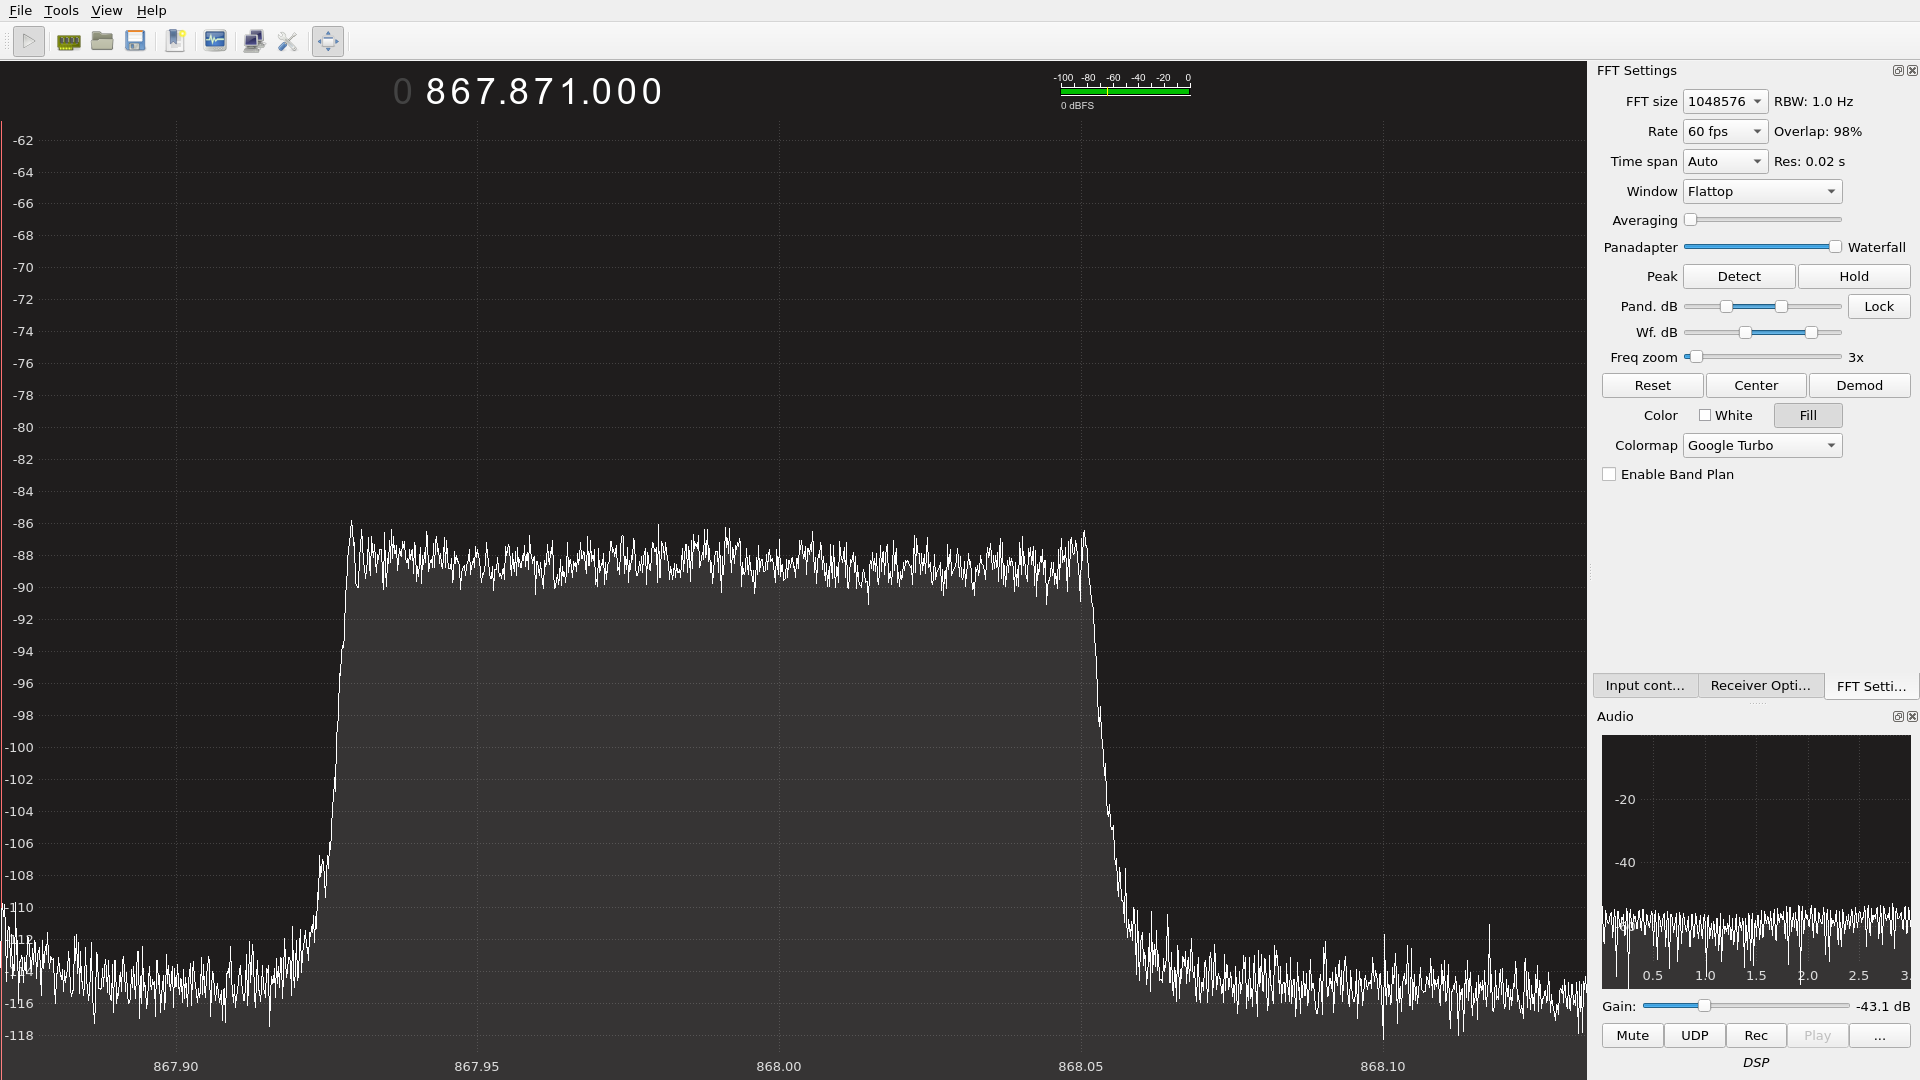
\includegraphics[width=0.9\textwidth]{research/frequency-graph-slave-response}
    \caption{\label{img:frequency-graph-slave-response}Widok spektrum częstotliwości podczas transmisji modułów SLAVE}
\end{figure}

\FloatBarrier
\subsection{\label{sect:iq-data-gqrx}Analiza zapisów danych I/Q zebranych \textsl{gqrx}} Ponieważ wykresy obserwowane
bezpośrednio w~oprogramowaniu \textsl{gqrx} nie pozwalały na analizę przesyłanych transmisji z~modułów, wykorzystana
została funkcja zapisu rejestrowanych danych do postaci I/Q (ang. \textsl{In-phase and quadrature components}) do plików
RAW. W~celu późniejszej analizy danych wykonane zostały 3~zapisy pełnych wymian danych w~sieci w~różnych konfiguracjach,
z~parametrami modułów ustawionych na podstawowych wartościach z~wyjątkiem Spreading Factor. Parametr ten ustawiony
został na wartość maksymalną (SF12, 12 bitów na symbol), tak aby uzyskać najlepsze szanse na analizę transmisji.

Dane I/Q to metoda opisu wielkości i~danych fazowych rejestrowanego sygnału, gdzie falę sinusoidalną można przedstawić
w~formie współrzędnych biegunowych \cite{ni-iq-data} korzystając z~równania:
\begin{equation}
    f(t) = A\cos{2\pi{ft}+\varphi}
\end{equation}
Zarejestrowane w~ten sposób dane (sinusoidę z~modulacją) można rozłożyć na dwie sinusoidy z~modulacją amplitudy, które
przesunięte są względem siebie w~fazie o ${\pi}/2$ radianów (90 stopni). Zarejestrowaną falę można wówczas przedstawić
w~złożonym układzie współrzędnych kartezjańskich, w~postaci składowych rzeczywistej i~urojonej, korzystając z~równań:
\begin{equation}
    I(t) = A\cos{\varphi}\cos{2\pi{ft}} \quad\text{(Składowa rzeczywista)}
\end{equation}
\begin{equation}
    Q(t) = A\sin{\varphi}\sin{2\pi{ft}} \quad\text{(Składowa urojona)}
\end{equation}

Korzystając z~zarejestrowanych zapisów, gdzie każdy miał długość około 25 sekund i~składał się z~około 25 milionów
próbek (związane z~ustawionym oknem FFT, milion próbek na sekundę) wykonana została ich analiza w~środowisku MATLAB.
Napisana została funkcja pozwalająca na generowanie spektrogramów pełnego zarejestrowanego sygnału oraz spektrogramów
zbliżenia na konkretne, wyznaczone, elementy. Kod źródłowy przedstawiony został na listingach
\ref{lst:matlab-spectrogram-zoom-1}, \ref{lst:matlab-spectrogram-zoom-2} oraz \ref{lst:matlab-spectrogram-zoom-3}
(przedstawiają kolejno: argumenty wejściowe funkcji, właściwe generowanie spektrogramów oraz funkcje pomocnicze do
ładowania danych z~plików RAW i~eksportu wygenerowanych wykresów).

\lstinputlisting[
    language=matlab,
    linerange={3-12},
    caption={Funkcja do analizy danych I/Q w~MATLAB -- argumenty wejściowe},
    label={lst:matlab-spectrogram-zoom-1},
    float=htbp
]{gqrx-spectrograms/spectrogramzoom.m}

\lstinputlisting[
    language=matlab,
    linerange={14-40},
    caption={Funkcja do analizy danych I/Q w~MATLAB -- generowanie pełnego spektrogramu oraz zbliżenia na wycinek},
    label={lst:matlab-spectrogram-zoom-2},
    float=htbp
]{gqrx-spectrograms/spectrogramzoom.m}

\lstinputlisting[
    language=matlab,
    linerange={43-57},
    caption={Funkcja do analizy danych I/Q w~MATLAB -- funkcje pomocnicze},
    label={lst:matlab-spectrogram-zoom-3},
    float=htbp
]{gqrx-spectrograms/spectrogramzoom.m}

Argumentami wejściowymi funkcji są: plik wejściowy (zawierający dane I/Q), ścieżka oraz nazwa pliku, gdzie wygenerowany
wykres ma zostać zapisany, zasięg próbek, na jakim ma zostać wykonane zbliżenie oraz dodatkowe parametry do funkcji
\texttt{spectrogram} -- wielkość okna, częstotliwość próbkowania, liczba nakładających się próbek, liczba punktów do
dyskretnej transformaty Fouriera.

\FloatBarrier
Funkcja pomocnicza, wykorzystywana do ładowania plików RAW, bazuje na równianach opisujących składowe rzeczywistą
i~urojoną. Plik zostaje otwarty w~momencie wywołania funkcji, a~jego zawartość odczytana w~postaci 32-bitowych wartości
zmiennoprzecinkowych (float32) z~najbardziej znaczącym bajtem jako pierwszym (ang. \textsl{Big endian}). Następnie
zawartość pliku ładowana jest do pamięci programu, modyfikując je do postaci złożonej (ang. \textsl{Complex}).

Generowanie spektrogramów wykorzystuje wbudowaną funkcję \texttt{spectrogram}. W~przypadku generowania wykresu dla
całego sygnału wykorzystywane są tylko argumenty wejściowe. Dodatkowo na podstawie wprowadzonych wartości, gdzie ma
zostać wykonane zbliżenie, na wykresie rysowane są linie pionowe na osi X. Korzystając z~długości (wielkości) tablicy
danych wejściowych, ustalane są ilość oraz rozstawienie podziałki. Natomiast w~przypadku wykresu zbliżenia, pierwszym
elementem jest wyznaczenie zakresu próbek, na podstawie których wygenerowany ma zostać spektrogram. Korzystając z~tych
dodatkowych zmiennych oraz pozostałych argumentów wejściowych generowany jest spektrogram zbliżenia. Ostatnim krokiem
w~funkcji jest eksport wykresu do pliku. Wykorzystywana jest do tego zaimplementowana funkcja pomocnicza
\texttt{exportfigure}. Zdefiniowane w~niej zmienne wykorzystywane są do zachowania poprawnych proporcji, tak aby wykres
miał największą możliwą czytelność.

\FloatBarrier
Korzystając z~zaimplementowanej funkcji, wygenerowane zostały spektrogramy jednego z~zarejestrowanych sygnałów, stosując
zwiększające przybliżenie, w~celu uzyskania jak najlepszego widoku na pojedynczą transmisję. Wygenerowane wykresy
przedstawione zostały przedstawione na rys. \ref{img:signal1-level1}, \ref{img:signal1-level2}, \ref{img:signal1-level3}
oraz \ref{img:signal1-level4} (zbliżenia w~czasie 2.5s a 6s, pokazujące 3~transmisje, do 3.6s a 4.6s, pokazując
dokładniej 1~transmisję).

\begin{figure}[!htbp]
    \centering
    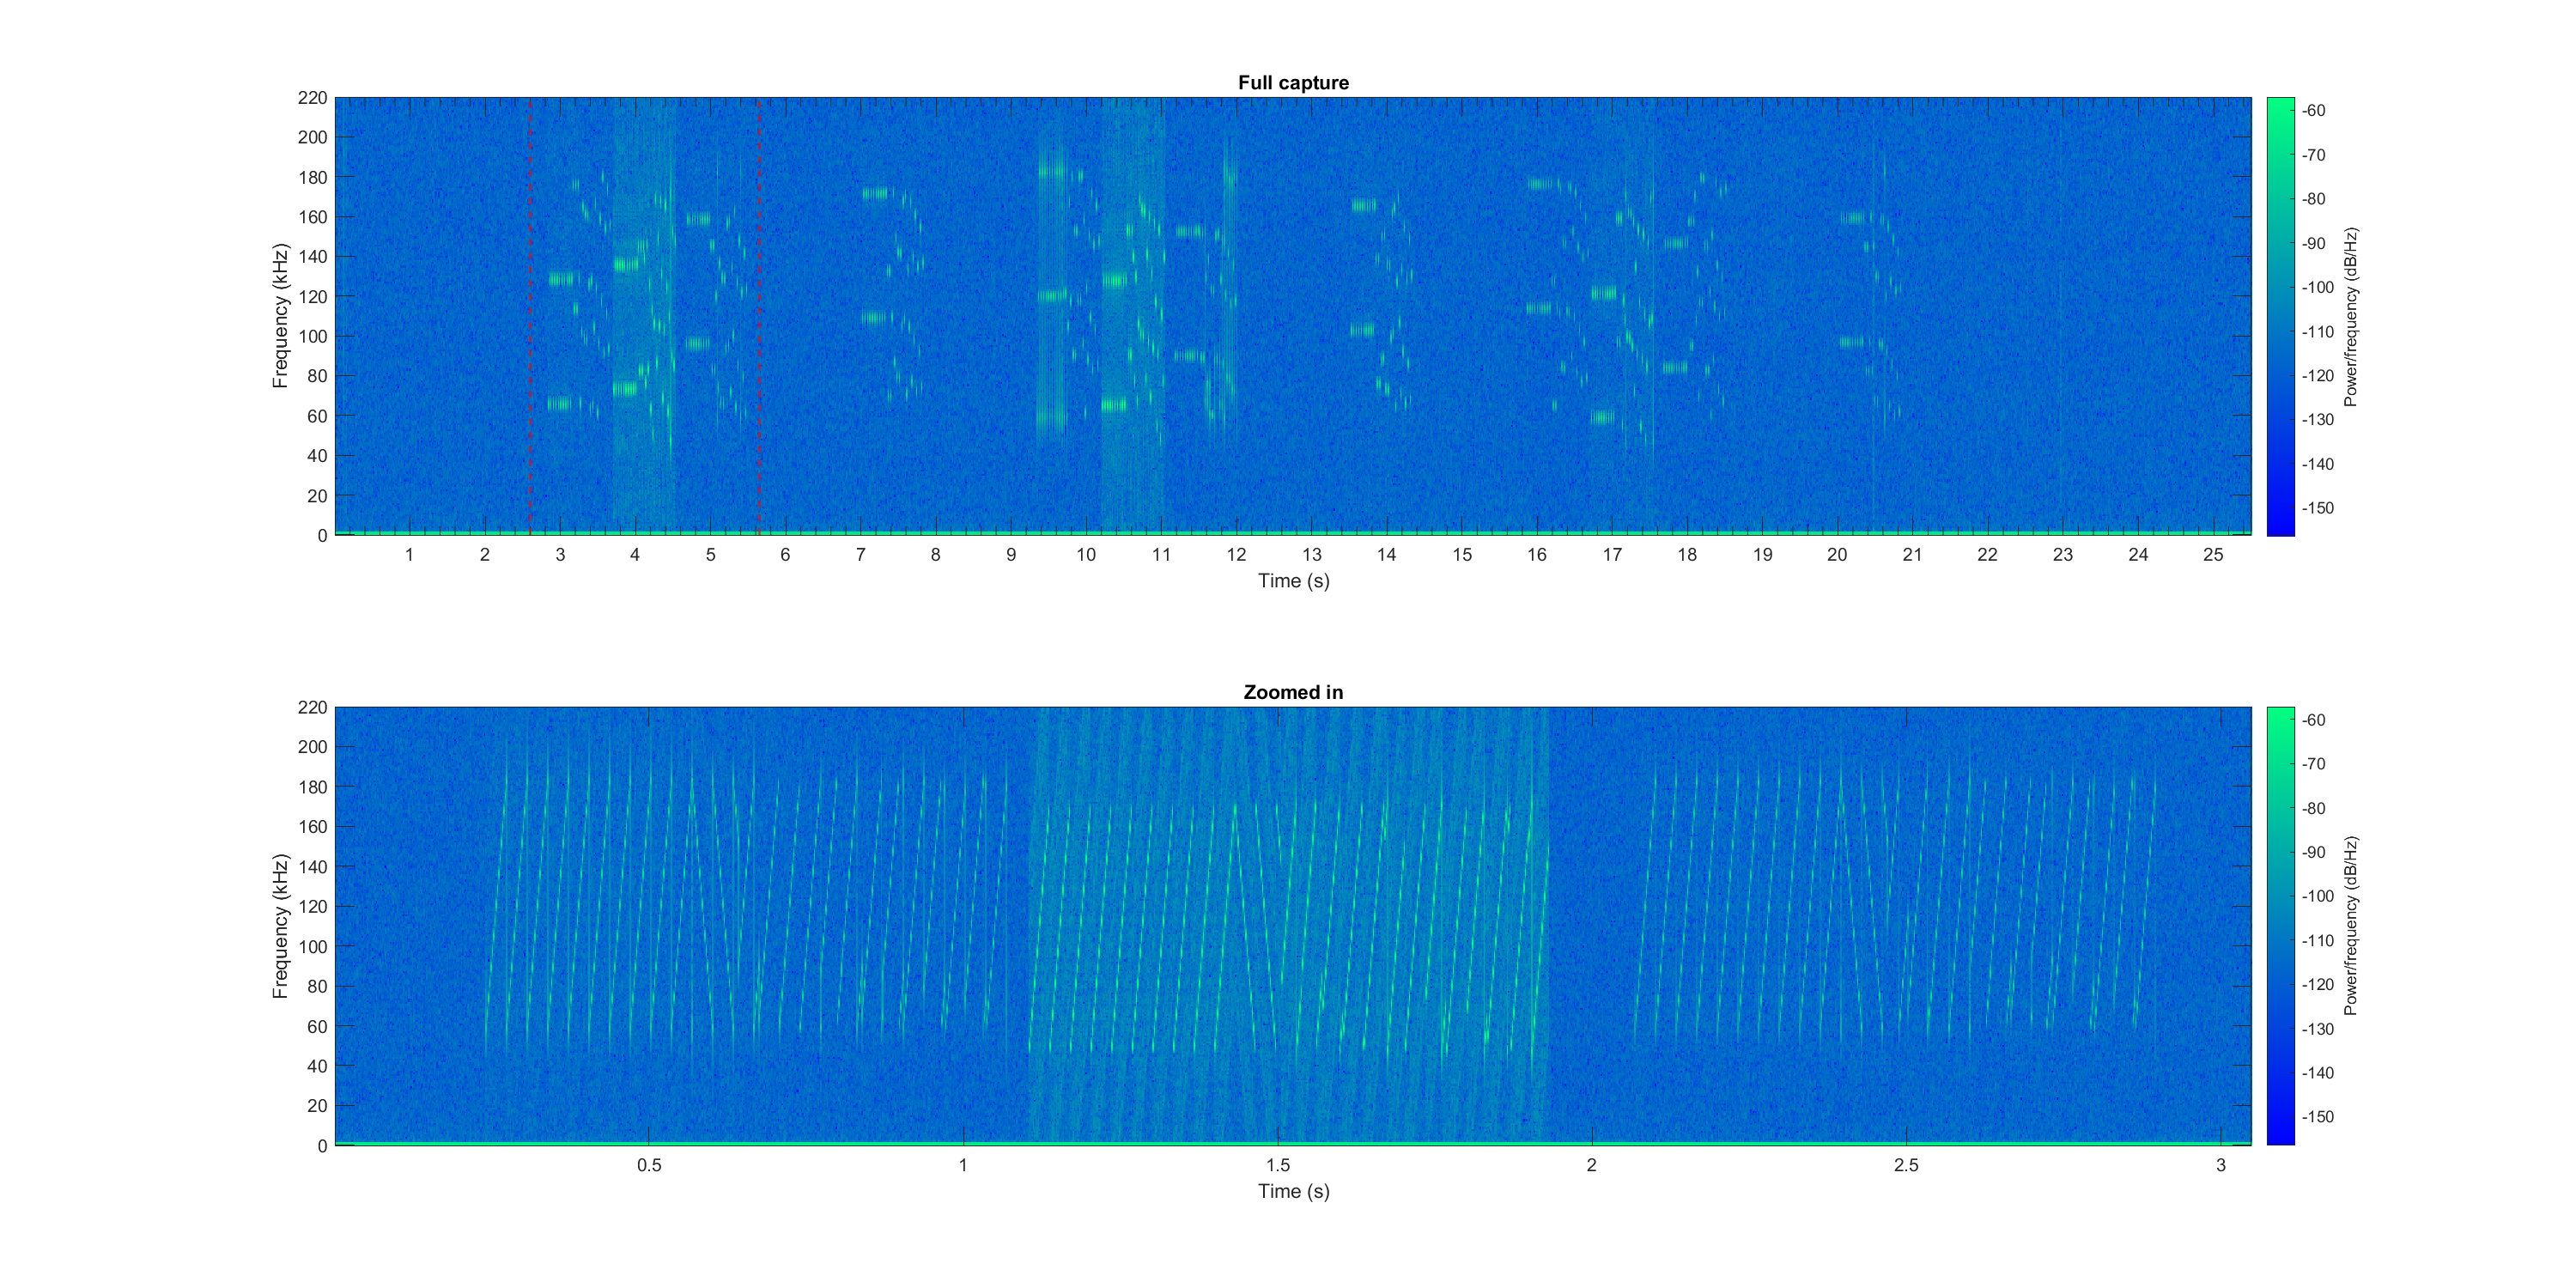
\includegraphics[width=\textwidth]{research/gqrx/zoom-win1024-sig1-lvl1}
    \caption{\label{img:signal1-level1}Spektrogram sygnałów z~pierwszej próbki wraz ze zbliżeniem między 2.5s a 5.5s}
\end{figure}

\begin{figure}[!htbp]
    \centering
    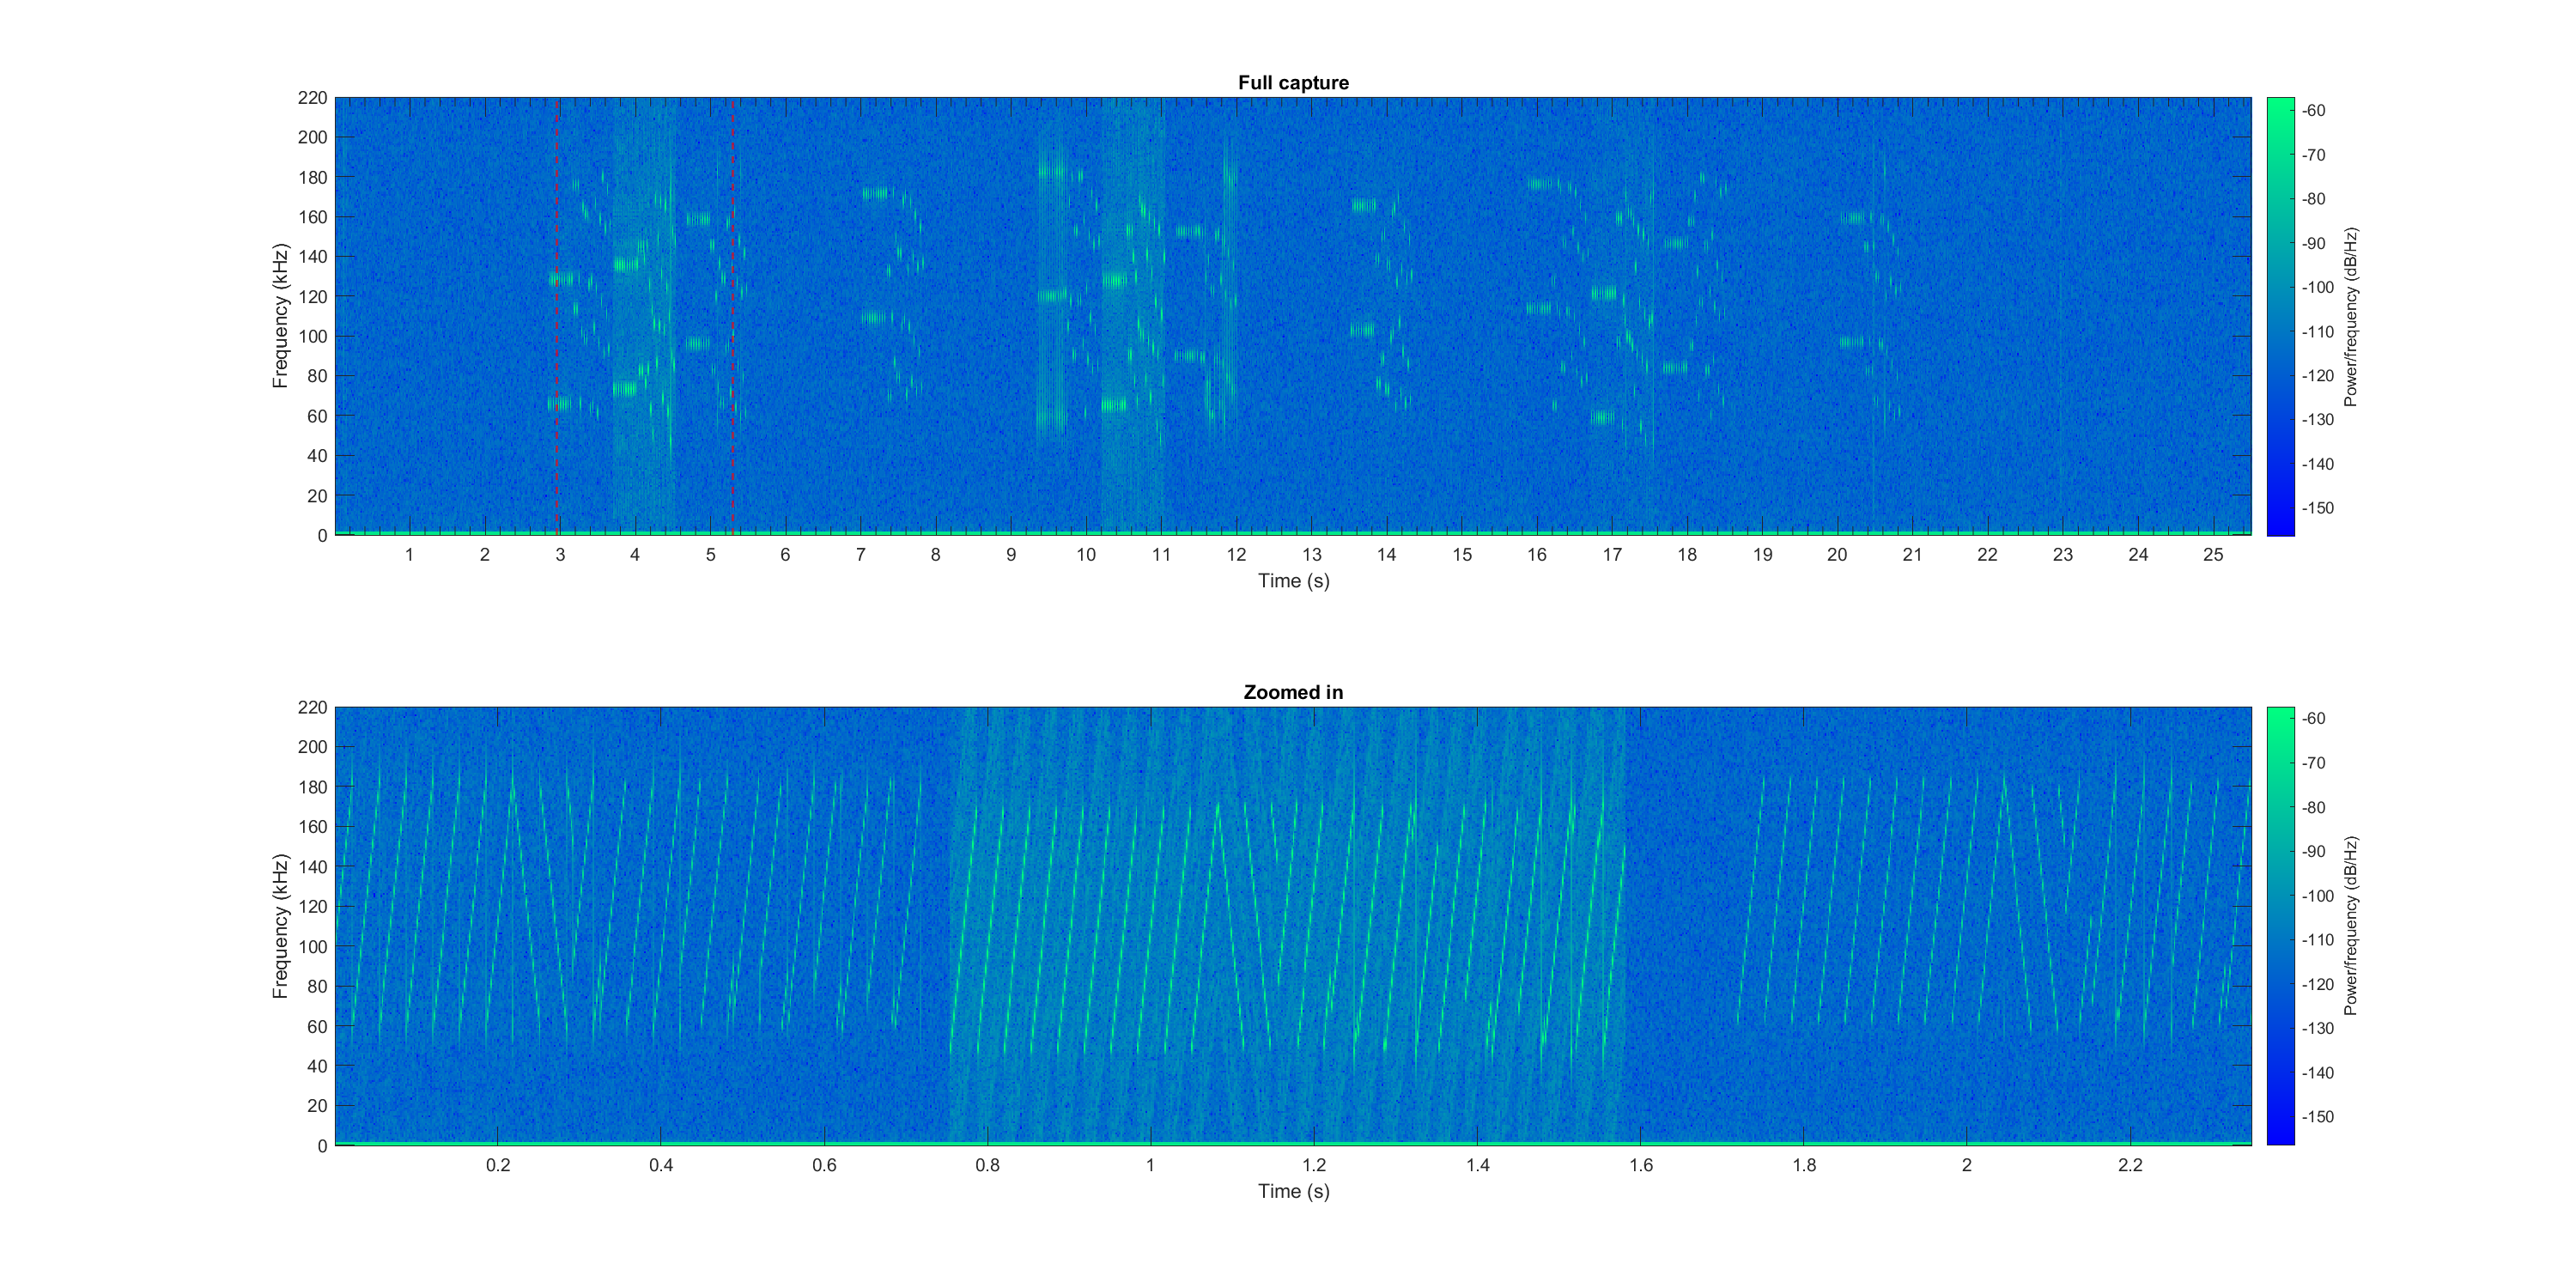
\includegraphics[width=\textwidth]{research/gqrx/zoom-win1024-sig1-lvl2}
    \caption{\label{img:signal1-level2}Spektrogram sygnałów z~pierwszej próbki wraz ze zbliżeniem między 3s a 5.1s}
\end{figure}

\begin{figure}[!htbp]
    \centering
    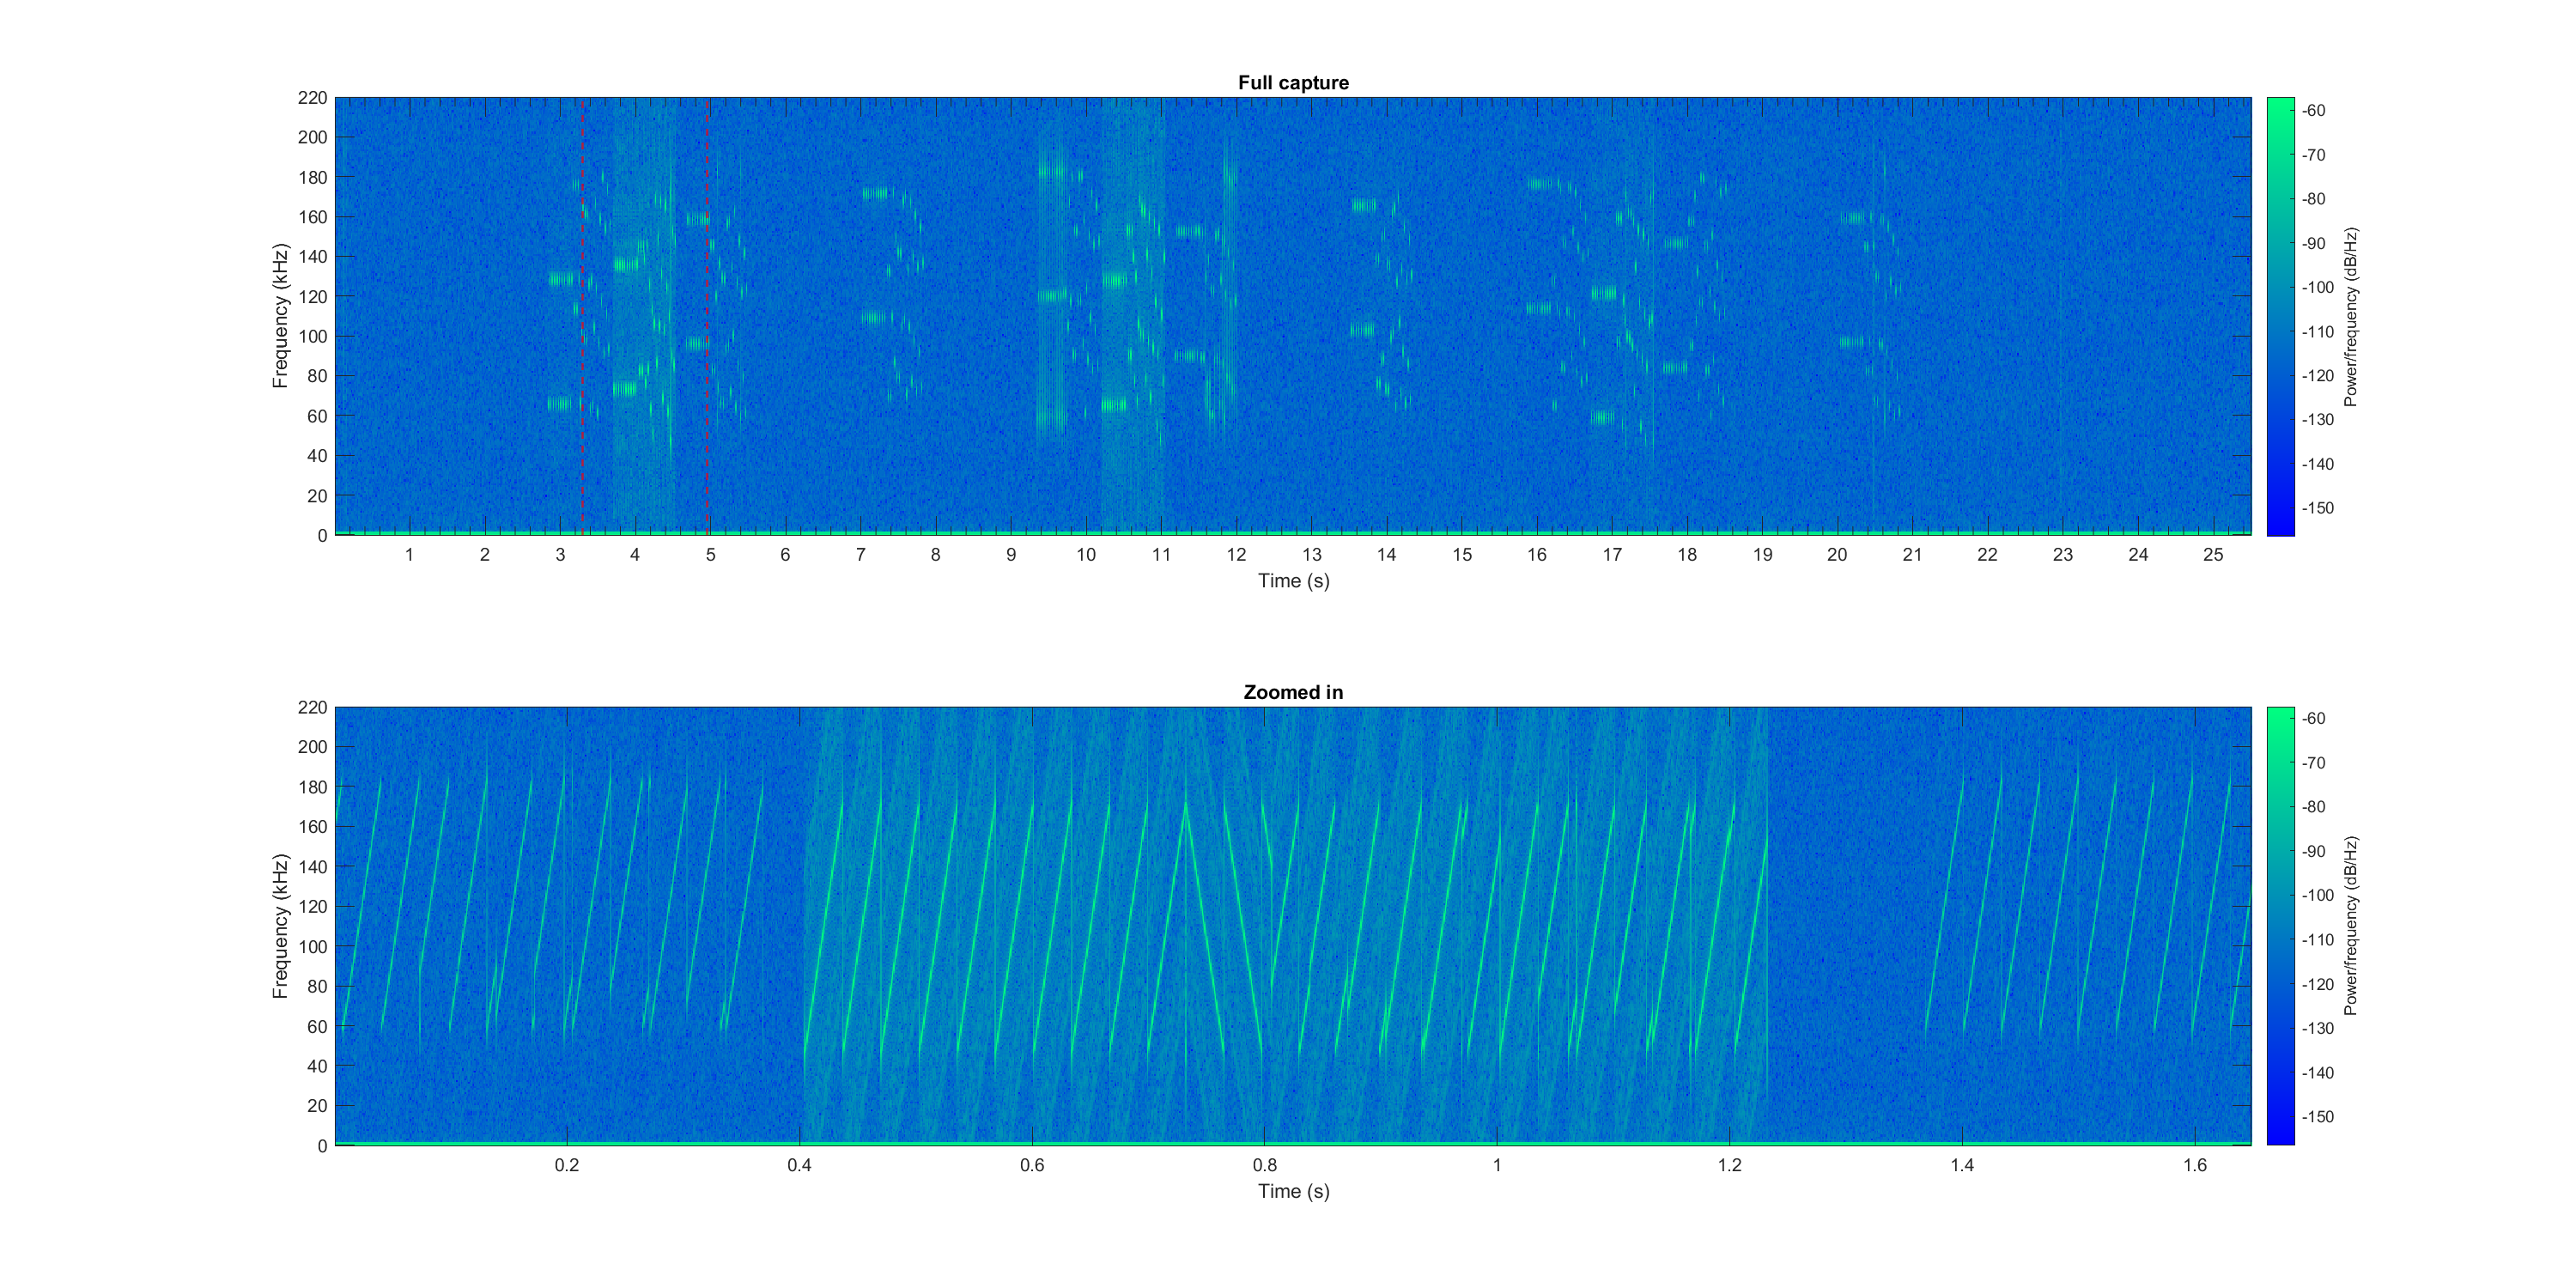
\includegraphics[width=\textwidth]{research/gqrx/zoom-win1024-sig1-lvl3}
    \caption{\label{img:signal1-level3}Spektrogram sygnałów z~pierwszej próbki wraz ze zbliżeniem między 3.4s a 5s}
\end{figure}

\begin{figure}[!htbp]
    \centering
    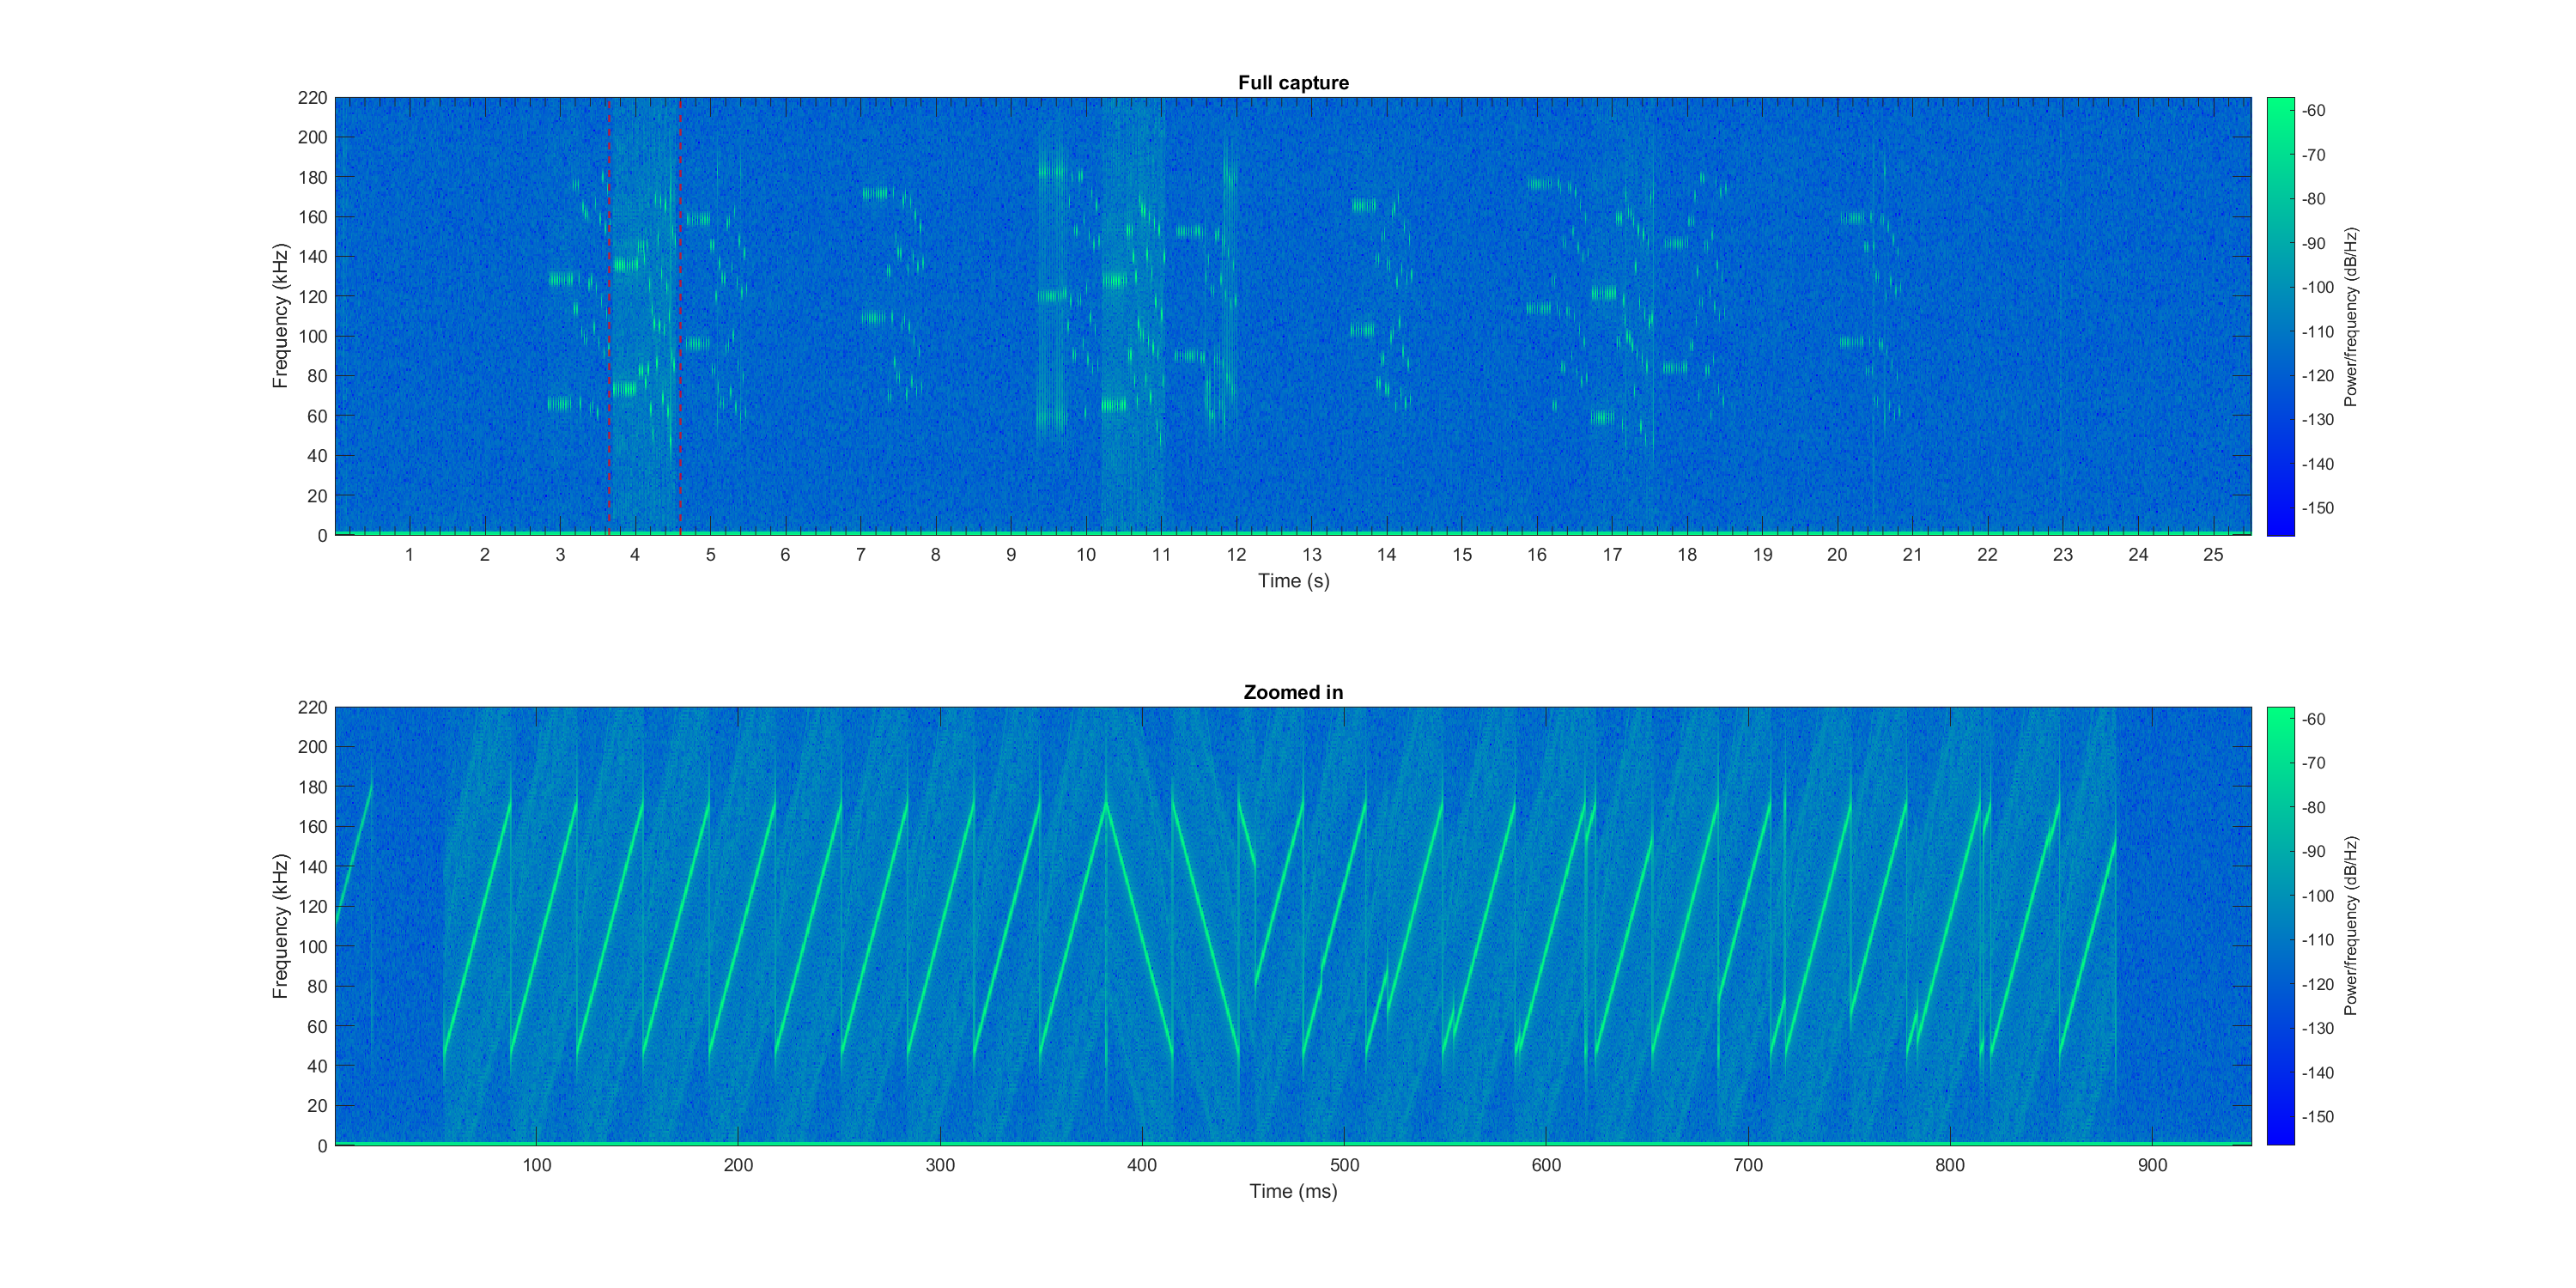
\includegraphics[width=\textwidth]{research/gqrx/zoom-win1024-sig1-lvl4}
    \caption{\label{img:signal1-level4}Spektrogram sygnałów z~pierwszej próbki wraz ze zbliżeniem między 3.6s a 4.6s,
        widoczna jedna transmisja}
\end{figure}

Na podstawie wygenerowanych spektrogramów możliwe było przeanalizowanie jednej pełnej ramki transmisji danych. Dzięki
uzyskanemu dużemu przybliżeniu na analizowany sygnał możliwe było wyznaczenie granic poszczególnych elementów ramki
LoRa. Przedstawione zostało to na rys. \ref{img:signal2-zoomed-analysis} oraz \ref{img:signal3-zoomed-analysis}
(odpowiednio dla fragmentu z~zarejestrowanych próbek drugiej oraz trzeciej).

\begin{figure}[!htbp]
    \centering
    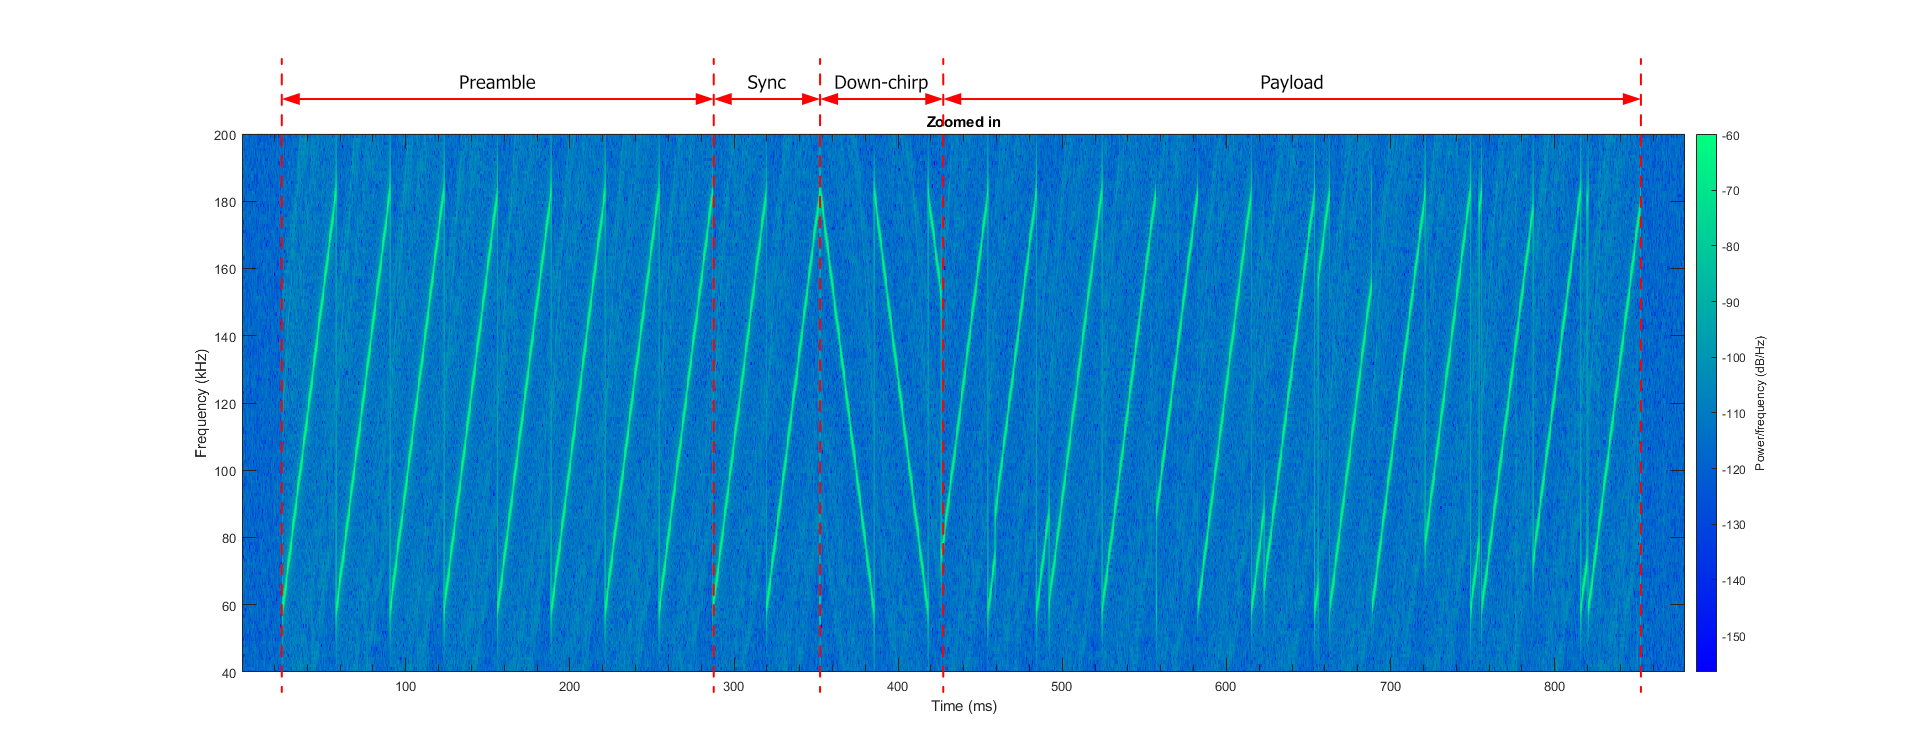
\includegraphics[width=\textwidth]{research/signal2-zoomed-analysis}
    \caption{\label{img:signal2-zoomed-analysis}Fragment drugiej próbki sygnału z~oznaczonymi poszczególnymi elementami
        ramki LoRa}
\end{figure}

\begin{figure}[!htbp]
    \centering
    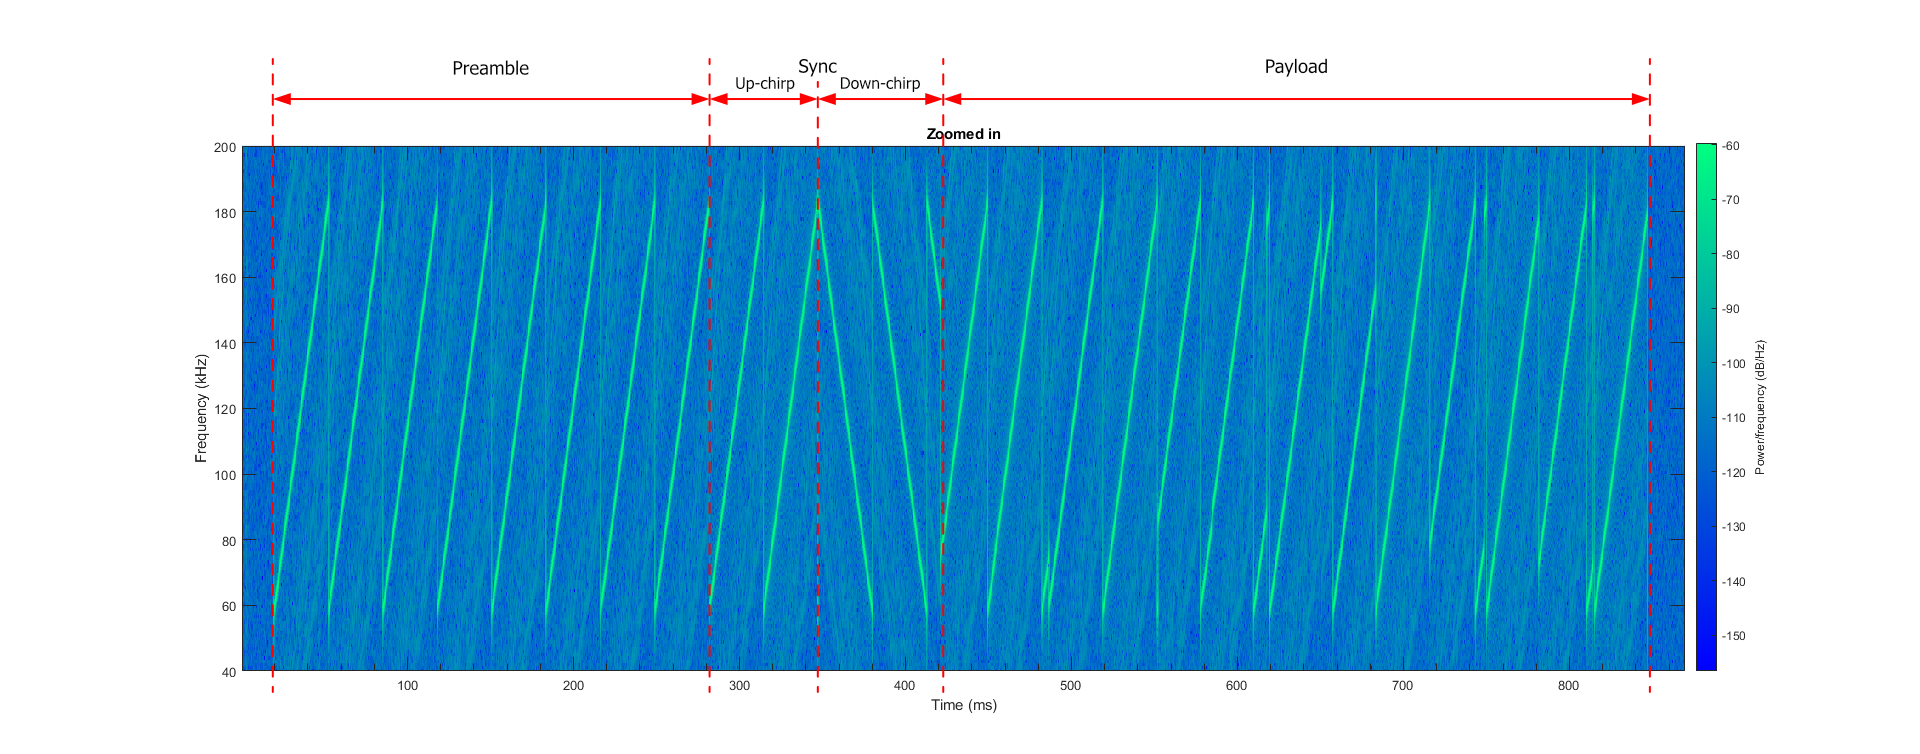
\includegraphics[width=\textwidth]{research/signal3-zoomed-analysis}
    \caption{\label{img:signal3-zoomed-analysis}Fragment trzeciej próbki sygnału z~oznaczonymi poszczególnymi elementami
        ramki LoRa}
\end{figure}

\FloatBarrier
Na przedstawionych fragmentach spektrogramów widoczne są różnice, pokazujące, że możliwe jest w~pewnym stopniu
rozróżnienie elementów transmisji. Są one widoczne tylko w~częściach oznaczonych jako "Payload" na wygenerowanych
wykresach, ponieważ tylko te elementy są zmienne w~każdej transmisji -- zawierają nagłówek, właściwe przesyłane dane
oraz kod CRC (ang. \textsl{Cyclic Redundancy Check}, służący wykrywaniu potencjalnych błędów w~transmisji). Pozostałe
elementy są elementami stałymi dla każdej ramki: preambuła (której długość ustawiona została na 8~symboli) -- pozwala
innym elementom sieci na wykrycie początku transmisji ramki, a~także dodatkowe symbole up-chirp oraz down-chirp --
w~sumie 4.25 symbolu, służące synchronizacji, aby mieć jak największą pewność, że dane, które mają zostać przesłane, nie
zostaną w~żaden sposób zniekształcone przez ew. przesunięcia w~czasie.

Ponieważ każda ramka LoRa zawiera kodowanie, możliwe jest jedynie rozróżnienia pojedynczych ramek między sobą, jednakże
nie jest już możliwe, korzystając wyłącznie ze spektrogramów, rozpoznanie co w~danym momencie jest przesyłane.
W~zaprezentowanych ramkach z~dwóch różnych próbek widać pewne różnice w~przesyłanych symbolach, jednakże tylko na
podstawie tego nie jest możliwe pokazanie, które symbole przedstawiają konkretne bity przesyłanych wiadomości.


\chapter{\label{ch:summary}Podsumowanie}
Celem pracy było zaprojektowanie, zaimplementowanie oraz weryfikacja hipotezy -- zbadanie możliwości zbudowania
prywatnej sieci czujnikowej bazującej na standardzie LoRa. W~ramach tego zapoznano się z~podstawami standardu:
działaniem modulacji, elementami składowymi przesyłanej ramki oraz parametrami wpływającymi na transmisję. Opisany
został proces przygotowania środowiska do tworzenia oprogramowania, kroki wymagane do zaczęcia pracy, wykorzystane
biblioteki oraz ograniczenia związane z~wybraną platformą. Ponadto przedstawione zostały elementy składające się na
całość implementowanego oprogramowania -- części dedykowane dla modułów pracujący w~budowanej sieci oraz modułu
wpierającego działanie systemu (serwera sieciowego do prezentacji danych). W~pracy przedstawione zostały także
przeprowadzone badania, które pozwoliły na określenie możliwości budowania sieci czujnikowych opartych o~standard LoRa.

W~ramach części projektowej (implementacji sieci) napisane zostało oprogramowanie, które pozwoliło na komunikację na
płytki rozwojowe STM32 Nucleo64 L152 wyposażone w~moduły LoRa. Oprogramowanie zawiera elementy, które pozwoliły na
weryfikowanie przesyłanych danych, zbieranie pomiarów oraz wyznaczanie z~nich średniej kroczącej, w~celu wyeliminowania
chwilowych znacznych zmian w~otoczeniu pracy sieci. Ponadto zaimplementowane zostało oprogramowanie na moduł serwera
sieciowego, który mógł odbierać dane z~modułu MASTER sieci LoRa. W~tym celu wykorzystana została zakodowana transmisja
przez magistralę I2C, która pozwalała na wykrywanie błędów w~transmisji danych. Zaimplementowana strona internetowa jest
bardzo prostym narzędziem pozwalającym na przeglądanie danych zbieranych przez sieć. Element ten mógłby zostać znacznie
ulepszony przez wykorzystanie innego typu sprzętu. Jednakże wybrana metoda pozwoliła na pokazanie, że nawet bardzo małe
urządzenia, które mogą działać na zasilaniu bateryjnym, mogą zostać z~sukcesem wykorzystane do takiego zadania.

W~ramach badań zweryfikowana została postawiona hipoteza -- czy możliwe jest zbudowanie prywatnej sieci czujnikowej
bazującej na standardzie LoRa. Przeprowadzone badania pozwoliły na zapoznanie się z~wyglądem przesyłanej ramki,
weryfikację działania sieci (w celu sprawdzenia stopnia błędów w~przesyłaniu wiadomości z~danymi), sprawdzenie
skutecznego zasięgu komunikacji oraz przepustowości, a~także poboru prądu oraz możliwości wykorzystania zasilania
bateryjnego do podtrzymania modułów sieci. Otrzymane wyniki badań pozwoliły na określenie, że standard LoRa może zostać
wykorzystany w~przypadku sieci prywatnych, projektowanych na mniejszą skalę.

W~przyszłości możliwe byłoby rozwinięcie oraz usprawnienie działania zaimplementowanego rozwiązania. Jednym z~elementów
byłoby zmiana modułu, sprzętu odpowiedzialnego za funkcję serwera sieciowego do zbierania danych. Możliwe byłoby
zastosowanie rozwiązania wyposażonego w~bazę danych. Pozwoliłoby to na zapisywanie zbieranych danych w~celu
dokładniejszej obróbki oraz bardziej przejrzystej prezentacji ich w~oparciu także o~dane historyczne, np. poprzez
wyświetlanie użytkownikowi wykresów pokazujących zmiany w~czasie. Zmiana wykorzystanego sprzętu mogłaby też pozwolić na
usprawnienie działania sieci czujnikowej -- zwiększenie skutecznego zasięgu komunikacji lub zmniejszenie stopnia błędu
w~transmisjach na większych dystansach.

\bibliografia

% Wykaz symboli i skrótów - patrz opis w tekście przykładowym
% \acronymslist
% Spis rysunków
\listoffigures
% Spis tabel
\listoftables
% Załączniki (plik appendices.tex)
% \easyappendices
\end{document}

